% ------------------------------------------------------------------------
% LaTeX deliverable template for SeaClear2.0 project
% by Lucian Busoniu, 10 Mar 2020 for SeaClear
% modified by Bart De Schutter, March 5, 2023 for SeaClear2.0
% modified by Vicu-Mihalis Maer, April 25, 2024 for SeaClear2.0 updated look
% modified by Nobuaki Aoki, Nov 14, 2025 for the new EU MISSIONS template look
% Known issues:
% - manual editing of appendix indices is required
% ------------------------------------------------------------------------

%%%%%%%%%%%%%%%%%%%%%%%%%%%%%%%%%%%%%%%%%%%%%%%%
% Deliverable properties - define these
% Only items that appear more than once are here, otherwise define them in-place in the text
\newcommand\dnumber{D5.2\xspace}                     % WARNING: replace "x.x"
\newcommand\dtitle{Report on Smart Grapple Software Framework\xspace}         % WARNING: replace "Deliverable title"
\newcommand\ddate{30/12/2025\xspace}             % WARNING: replace "day/month/year"
\newcommand\dversion{V1.0\xspace}                    % WARNING: replace "x.x"
\newcommand\dtype{R}             % WARNING: select R, DEM, OTHER, or DMP
\newcommand\dlevel{PU\xspace}      % WARNING: select PU, C-UE/EU-C, or SEN
\newcommand\wpnumber{WP5\xspace}                     % WARNING: replace "x"
\newcommand\wptitle{Control Overhaul\xspace}                 % WARNING: replace "WP title"
\newcommand\authorname{Stefan Sosnowski\xspace}   % WARNING: replace "Initials, Last Name"
\newcommand\authoremail{sosnowski@tum.de\xspace}     % WARNING: replace "email@domain.com"
%\newcommand\authorphone{00000000000000000\xspace}        % WARNING: replace "00000000000000000"
\newcommand\authorinstitution{TUM\xspace} % WARNING: replace "Name of institute"
\newcommand\dlead{TUM\xspace}           % WARNING: replace "Lead institution"

%\newcommand{\bds}[1]{\textcolor{red}{Comment: #1}}
\newcommand{\bds}[1]{}
\newcommand{\ian}[1]{#1}
\newcommand{\hamish}[1]{#1}
\newcommand{\revision}[1]{#1}

%%%%%%%%%%%%%%%%%%%%%%%%%%%%%%%%%%%%%%%%%%%%%%%%
% Document customization -- there should be no need to touch this
\documentclass[a4paper,11pt]{article}

\usepackage[utf8]{inputenc}
\usepackage[T1]{fontenc}

\usepackage[sfdefault,lf]{carlito}     % calibri look-alike font
\usepackage{cite}
\usepackage{graphicx}
\usepackage{wrapfig}
\usepackage{fancyhdr}
\usepackage{amsmath,amssymb}
\DeclareMathOperator*{\argmin}{arg\,min}
\DeclareMathOperator*{\argmax}{arg\,max}
\usepackage{bm}
\usepackage{algorithm}
\usepackage{algpseudocode}
\usepackage{color}
\usepackage{colortbl, tabularx}
\usepackage{multirow}
\usepackage{times}
\usepackage{xspace}
\usepackage[export]{adjustbox}
\usepackage{mathtools}
\usepackage{datetime}
\usepackage{soul}
\usepackage{tabularx} % Add this in your preamble
\usepackage{booktabs} % For better table lines
\usepackage{siunitx}  % For nice units and numbers (optional but recommended)
\usepackage{subcaption}
\usepackage{svg}
\usepackage{tikz}
\usetikzlibrary{shapes, arrows.meta, positioning, calc}
\usepackage{tocloft}
\usepackage{eso-pic}
\PassOptionsToPackage{hyphens}{url}
\usepackage{hyperref}
\hypersetup{
    colorlinks=true,% false: boxed links; true: colored links
    citecolor=teal,% colour of links to bibliography
    linkcolor=purple,% colour of internal links
    urlcolor=cyan,% colour of external links
    filecolor=magenta,% colour of file links
    pdftitle={SeaClear2.0-D4.2},% pdf title
    }
\PassOptionsToPackage{hyphens}{url}\usepackage{hyperref}

\usepackage[capitalise]{cleveref}% cref

\usepackage[acronym]{glossaries}
\makeglossaries
\loadglsentries{glossary.tex}

\renewcommand{\cftsecleader}{\textbf{\cftdotfill{\cftdotsep}}}
\renewcommand{\cftsecfont}{\Large\bfseries}           % \section font in ToC
\renewcommand{\cftsubsecfont}{\large}        % \subsection font in ToC

\PassOptionsToPackage{hyphens}{url}\usepackage{hyperref}
%\usepackage[bookmarks=false,pdfstartview=Continuous]{hyperref}
%\usepackage{tocloft}
\ddmmyyyydate

\usepackage[a4paper, top=25.4mm, bottom=50mm, left=25.4mm, right=25.4mm, foot=35pt]{geometry}

% text customization
\setlength\parindent{0pt}
\setlength\parskip{0.75em}
\let\oldsection\section
\renewcommand\section{\clearpage\oldsection}

% Table customization
\definecolor{tableblue}{rgb}{0,0.44,0.75}
\definecolor{tabletan}{rgb}{0.93,0.92,0.88}
\setlength{\tabcolsep}{10pt}
\renewcommand{\arraystretch}{1.4}
% \setlength\arrayrulewidth{1.5pt}

%  Header/footer definitions
\renewcommand{\headrulewidth}{0pt}
\lhead{}
\chead{
{\small
\begin{tabularx}{\textwidth}{|c|X|l|}
  \hline
  \multirow{2}{*}{\begin{minipage}[b]{11mm}\vspace*{0.5mm}
\includegraphics[width=11mm]{img/SC2_Logo.pdf}\end{minipage}}  & \multicolumn{2}{l|}{\textbf{\dnumber:} \dtitle}\\ \cline{2-3}
  &  \textbf{\wpnumber:} \wptitle & \textbf{Version:} \dversion \\ \cline{2-3}
  101093822   & \textbf{Author(s):} \authorname (\authorinstitution) Nicolas Hoischen (TUM), Tzu-Yuan Huang (TUM), Anastasio Natsakis (UTC)
  & \textbf{Level:} \dlevel \\\hline
\end{tabularx}
}
}
\rhead{}
\renewcommand{\footrulewidth}{0pt}
\setlength{\footskip}{0.5cm}
\lfoot{}
\cfoot{%
    \vspace{-2mm}
    \parbox{\textwidth}{\centering
        \fontsize{8pt}{9pt}\selectfont
        SeaClear2.0 is co-funded by the European Union under the Horizon Europe Programme (Grant Agreement 101093822). Views and opinions expressed herein are those of the author(s) and do not necessarily reflect those of the European Union or European Climate, Infrastructure and Environment Executive Agency (CINEA). Neither the European Union nor the granting authority can be held responsible for them
    }
    
    \vspace{0.2cm}
    \makebox[\textwidth][r]{
        \fontsize{9pt}{9.6pt}\selectfont
        \textbf{\textcopyright \ European Union, 2021. All rights reserved}
        \hspace*{2cm}
    }\\%
    \vspace{0.1cm}
    \makebox[\textwidth][r]{
        \normalsize\thepage
        \hspace*{2cm}
    }
}
\rfoot{}

\AddToShipoutPictureBG{
    \begin{tikzpicture}[remember picture, overlay]
        \node[anchor=south, inner sep=0]%
            at (current page.south)
            {
\includegraphics[width=\paperwidth]{img/bottom_split_logo.png}};
    \end{tikzpicture}
}
% \makebox[\textwidth][c]{
%     
\includegraphics[width=6.56cm]{img/Co-foundedByTheEU.png} \fontsize{8pt}{8pt}\selectfont SeaClear2.0 is co-funded by the European Union under the Horizon Europe Programme (Grant Agreement 101093822). Views and opinions expressed herein are those of the author(s) and do not necessarily reflect those of the European Union or European Climate, Infrastructure and Environment Executive Agency (CINEA). Neither the European Union nor the granting authority can be held responsible for them \\
%      \centering\thepage}

% TOC customization
\renewcommand{\contentsname}{Table of Contents}
%\newcommand{\cftchapterleader}{\hrulefill}
\newcommand{\Mat}[1]{\mathbf{\MakeUppercase{#1}}}
\renewcommand{\vec}[1]{\boldsymbol{\mathbf{\MakeLowercase{#1}}}}
\newcommand{\expect}{\mathbb{E}}
\newcommand{\abs}[1]{\left|{#1}\right|}
\newcommand{\norm}[1]{\left\| {#1} \right\|}
\begin{document}
%%%%%%%%%%%%%%%%%%%%%%%%%%%%%%%%%%%%%%%%%%%%%%%%%%%%%%%%%%%%%%%%%%%%%%%%%%%%%%
% Title page
%%%%%%%%%%%%%%%%%%%%%%%%%%%%%%%%%%%%%%%%%%%%%%%%%%%%%%%%%%%%%%%%%%%%%%%%%%%%%%
% \AddToHookNext{shipout/background}{
%   \begin{tikzpicture}[remember picture,overlay]
%   \node at (current page.north west) {
%     
\includegraphics[width=13.79cm]{img/TopLeftOrn.png}
%   };
%   \end{tikzpicture}
% }
% \xdef\exacttopmargin{\the\dimexpr2em+\headsep+\headheight+\topmargin+1in\relax}%
% \reversemarginpar\marginpar{
%     \vspace*{-\exacttopmargin}%
% 	\begin{flushright}
% 		
\includegraphics[width=13.79cm]{img/TopLeftOrn.png}
% 	\end{flushright}
% } 
%     \vspace*{-\exacttopmargin}%

% \begin{flushright}
% 	
\includegraphics[width=2.79cm]{img/SC2_Logo.pdf}\hspace*{-1cm}
% 	\end{flushright}
% \begin{flushright}
% 	
\includegraphics[width=2.79cm]{img/SC2_Logo.pdf}\hspace*{-1cm}
% 	\end{flushright}
 \begin{tikzpicture}[remember picture, overlay]
    \node[anchor=north east, inner sep=0, xshift=-0.5cm, yshift=-0.5cm]%
        at (current page.north east)
        {
\includegraphics[width=2.79cm]{img/SC2_Logo.pdf}};
\end{tikzpicture}
\begin{tikzpicture}[remember picture, overlay]
    \node[anchor=south, inner sep=0]
        at (current page.south)
        {
\includegraphics[width=\paperwidth]{img/BottomLogo.png}};
\end{tikzpicture}
%\rightline{
\includegraphics[width=30mm]{img/SC2_Logo.pdf}}

\begin{center}
\vspace{2cm}
\LARGE{\textbf{Scalable full-cycle marine litter remediation in the\\ Mediterranean: Robotic and participatory solutions}}
\vskip 0.7cm
\Huge{SeaClear2.0}
\end{center}
\vskip 1cm
\rightline{\url{https://www.seaclear2.eu}}
\vskip 1cm
{\Large
\leftline{\textbf{\dnumber}}
\leftline{\textbf{\dtitle}}
}
\leftline{\textbf{\wpnumber{} --- \wptitle}} \vskip 1cm
\rightline{\textbf{Grant Agreement no.~101093822}}\vskip .5em
{\color[HTML]{4F81BD}\rule{\textwidth}{1.5pt}}
\rightline{Lead beneficiary: \dlead}
\rightline{}
\rightline{Date: \ddate}
\rightline{Type: \dtype}
\rightline{Dissemination level: \dlevel}
\vfill

\begin{center}
    \fontsize{8pt}{7.5pt}\selectfont
    \parbox{\textwidth}{
        SeaClear2.0 is co-funded by the European Union under the Horizon Europe Programme (Grant Agreement 101093822). Views and opinions expressed are those of the author(s) and do not necessarily reflect those of the European Union or European Climate, Infrastructure and Environment Executive Agency (CINEA). Neither the European Union nor the granting authority can be held responsible for them.
    }
\end{center}

\vspace{0.1cm}

\leftline{
    \fontsize{9pt}{9.6pt}\selectfont 
    \textbf{\textcopyright \ European Union, 2021. All rights reserved}
}

\vfill
% \vspace{1cm}
% \begin{flushright}
%     
\includegraphics[width=11.09cm]{img/BottomRightOrn.png}\hspace*{-1.55cm}
% \end{flushright}
\thispagestyle{empty}
%%%%%%%%%%%%%%%%%%%%%%%%%%%%%%%%%%%%%%%%%%%%%%%%%%%%%%%%%%%%%%%%%%%%%%%%%%%%%%
% Document info page
%%%%%%%%%%%%%%%%%%%%%%%%%%%%%%%%%%%%%%%%%%%%%%%%%%%%%%%%%%%%%%%%%%%%%%%%%%%%%%
\pagebreak
\setlength\headheight{66pt}
\pagestyle{fancy}

\section*{Document information}\vspace*{-2mm}
%\addcontentsline{toc}{section}{Document information}

\begin{tabularx}{\textwidth}{|@{\ }l|@{\ }X|}
  \hline
  \textbf{Grant agreement no.}      & 101093822 \\ \hline
  \textbf{Acronym:}                 & SeaClear2.0 \\ \hline
  \textbf{Full title:}              & Scalable full-cycle marine litter remediation in the Mediterranean: Robotic and \mbox{participatory} solutions\\ \hline
  \textbf{Start date of the project}& 01/01/2023 \\ \hline
  \textbf{Duration of the project}  & 48 months \\ \hline
  \multicolumn{2}{|l|}{\quad}\\\hline
  \textbf{Deliverable}              & \dnumber: \dtitle \\ \hline
  \textbf{Work package}             & \wpnumber: \wptitle \\ \hline
  \textbf{Deliverable leader}       & \dlead \\ \hline
  \textbf{Delivery date}            & Contractual: 31/12/2025 \quad Actual: \ddate\\ \hline
  % WARNIJG: in the next lines replace $\square$ by \checkmark at the appropriate places
  \textbf{Status}                   & Draft $\square$  \qquad Final $\checkmark$ \\ \hline
  \textbf{Type}$^*$
                                    & R $\checkmark$ \qquad DEM $\square$ \qquad OTHER $\square$ \qquad DMP $\square$ \\\hline
  \textbf{Dissemination level}$^\dagger$ % <<< MODIFIED
                                    & PU $\checkmark$  \qquad C-UE/EU-C $\square$ \qquad SEN $\square$  \\ \hline
  \textbf{Author(s)}                & \authorname (\authorinstitution) \\
                                    & Nicolas Hoischen (\authorinstitution) \\
                                    & Tzu-Yuan Huang (\authorinstitution) \\
                                    & Anastasios Natsakis (UTC)\\
                                    & Hamish Grant (TUM) \\
                                    & Lucas De Oliveira e Silva (TUM) \\
                                    & Zara Zhotabayeva (TUM) \\ \hline
  \textbf{Responsible author}       & \authorname, email: \authoremail \\%, phone: \authorphone\\
                                    & \authorinstitution\\ \hline
  \textbf{Deliverable description}
  & Report on the perception and control approach that will be developed, based on the smart grapple design in T3.2, for localizing and precisely manipulating debris items under environmental disturbances. Including a holistic optimal control approach of the integrated USV - smart grapple system. This deliverable reflects work done in task T5.2 "Smart grapple sensing and control".
  \\ \hline
\end{tabularx}
%\vspace*{5cm}

\vspace{1cm}

\rule{5cm}{0.4pt}
\vspace{0.1cm} 

\noindent
\footnotesize 
$^1$ R = Document, report, DEM = demonstrator, OTHER: Software, technical diagram, etc. DMP = Data Management Plan \\
$^2$ PU = Public, C-UE/EU-C = EU Confidential under Decision 2015/444, SEN = Sensitive
\normalsize 


%%%%%%%%%%%%%%%%%%%%%%%%%%%%%%%%%%%%%%%%%%%%%%%%%%%%%%%%%%%%%%%%%%%%%%%%%%%%%%
% Version control page
%%%%%%%%%%%%%%%%%%%%%%%%%%%%%%%%%%%%%%%%%%%%%%%%%%%%%%%%%%%%%%%%%%%%%%%%%%%%%%

\section*{Document history}
%\addcontentsline{toc}{section}{Document history}

\begin{tabularx}{\textwidth}{|X|X|X|X|}
  \hline
  \rowcolor{tableblue}\textcolor{white}{\textbf{Name}}
  & \textcolor{white}{\textbf{Date}}
  & \textcolor{white}{\textbf{Version}}
  & \textcolor{white}{\textbf{Description}} \\ \hline
  Nicolas Hoischen    &   03/11/2025   & V0.1           & initial draft setup  \\\hline
  Stefan Sosnowski    &   28/11/2025    & V0.2           & final draft \\\hline
  Stefan Sosnowski    &   30/12/2025    & V1.0           & final version \\\hline
  % \hl{Initials, last name}    &   \hl{DD/MM/YYYY}    & V1.0           & \hl{what changed} \\\hline
\end{tabularx}

%%%%%%%%%%%%%%%%%%%%%%%%%%%%%%%%%%%%%%%%%%%%%%%%%%%%%%%%%%%%%%%%%%%%%%%%%%%%%%
% Disclaimer page
%%%%%%%%%%%%%%%%%%%%%%%%%%%%%%%%%%%%%%%%%%%%%%%%%%%%%%%%%%%%%%%%%%%%%%%%%%%%%%
\section*{Disclaimer of warranties}
%\addcontentsline{toc}{section}{Disclaimer of warranties}

This document has been prepared by SeaClear2.0 project partners as an account of work carried out within the framework of Grant Agreement no.~101093822.
Neither the Project Coordinator, nor any signatory party of the SeaClear2.0 Project Consortium Agreement, nor any person acting on behalf of any of them:
\begin{itemize}
\item makes any warranty or representation whatsoever, express or implied, with respect to the use of any information, apparatus, method, process, or similar item disclosed in this document, including merchantability and fitness for a particular purpose, that such use does not infringe on or interfere with privately owned rights, including any party's intellectual property; or
\item makes any warranty or representation whatsoever, express or implied, that this document is suitable to any particular user's circumstance; or
\item assumes responsibility for any damages or other liability whatsoever (including any consequential damages, even if the Project Coordinator or any representative of a signatory party of the Project Consortium Agreement, has been advised of the possibility of such damages) resulting from your selection or use of this document or any information, apparatus, method, process, or similar item disclosed in this document.
\end{itemize}

SeaClear2.0 is co-funded by the European Union under the Horizon Europe Programme (Grant Agreement 101093822). Views and opinions expressed are those of the author(s) and do not necessarily reflect those of the European Union or European Climate, Infrastructure and Environment Executive Agency (CINEA). Neither the European Union nor the granting authority can be held responsible for them.


%%%%%%%%%%%%%%%%%%%%%%%%%%%%%%%%%%%%%%%%%%%%%%%%%%%%%%%%%%%%%%%%%%%%%%%%%%%%%%
% TOC page
%%%%%%%%%%%%%%%%%%%%%%%%%%%%%%%%%%%%%%%%%%%%%%%%%%%%%%%%%%%%%%%%%%%%%%%%%%%%%%
\pagebreak

\tableofcontents
% Comment:
% please check and fix consistent use of initial caps in 
% titles of chapters and (sub)sections

%%%%%%%%%%%%%%%%%%%%%%%%%%%%%%%%%%%%%%%%%%%%%%%%%%%%%%%%%%%%%%%%%%%%%%%%%%%%%%
% Definitions and abbreviations page
%%%%%%%%%%%%%%%%%%%%%%%%%%%%%%%%%%%%%%%%%%%%%%%%%%%%%%%%%%%%%%%%%%%%%%%%%%%%%%
\section*{Definitions}
\addcontentsline{toc}{section}{Definitions}

\begin{itemize}
\setlength\itemsep{0em}
\item \textbf{Beneficiary:} A legal entity that is signatory of the EC Grant Agreement no.~101093822.
\item \textbf{Consortium:} The SeaClear2.0 Consortium, comprising the below-mentioned list of beneficiaries.
\item \textbf{Consortium Agreement:} Agreement concluded amongst SeaClear2.0 Beneficiaries for the implementation of the Grant Agreement.
\item \textbf{Grant Agreement:} The agreement signed between the beneficiaries and the EC for the undertaking of the SeaClear2.0 project (Grant Agreement no.~101093822).
% add as needed
\end{itemize}

Beneficiaries of the SeaClear2.0 Consortium are referred to herein according to the following abbreviations:
\begin{itemize}
\setlength\itemsep{0em}
\item \textbf{TU Delft:} TECHNISCHE UNIVERSITEIT DELFT
\item \textbf{DUNEA:} REGIONALNA AGENCIJA DUNEA
\item \textbf{Fraunhofer:} FRAUNHOFER GESELLSCHAFT ZUR FORDERUNG DER ANGEWANDTEN FORSCHUNG EV
\item \textbf{HPA:} HAMBURG PORT AUTHORITY
\item \textbf{ISOTECH}: ISOTECH LTD
\item \textbf{MDanchor}: M.\ DANCHOR LTD
\item \textbf{Subsea Tech:} SUBSEA TECH SAS
\item \textbf{TECNOSUB}: T\'{E}CNICAS Y OBRAS SUBACU\'{A}TICAS, SLU
\item \textbf{TUM}: TECHNISCHE UNIVERSITAET MUENCHEN
\item \textbf{UNIDU:} SVEUCILISTE U DUBROVNIKU
\item \textbf{UTC}: UNIVERSITATEA TEHNICA CLUJ-NAPOCA
\item \textbf{VEO}: VEOLIA PROPRETE
\item \textbf{VLPF}: VENICE LAGOON PLASTIC FREE
\end{itemize}

% \oldsection*{Abbreviations}
\addcontentsline{toc}{section}{Abbreviations}
\printglossary[type=\acronymtype,title={Abbreviations}]
% \begin{itemize}
% \setlength\itemsep{0em}
% \item \textbf{EC:} European Commission
% \item \textbf{GA:} Grant Agreement
% \item \textbf{WP}: Work Package
% \item \textbf{SGS}: Smart Grapple System
% \item \hl{Add more as needed}
% \end{itemize}
\vfill
\#MissionOcean \#EUMissions \#HorizonEU \#OceanCharter
%%%%%%%%%%%%%%%%%%%%%%%%%%%%%%%%%%%%%%%%%%%%%%%%%%%%%%%%%%%%%%%%%%%%%%%%%%%%%%
% Executive summary page
%%%%%%%%%%%%%%%%%%%%%%%%%%%%%%%%%%%%%%%%%%%%%%%%%%%%%%%%%%%%%%%%%%%%%%%%%%%%%%
\section*{Executive summary}
\addcontentsline{toc}{section}{Executive Summary}

This deliverable (D5.2) presents the software framework developed for the Smart Grapple system within the SeaClear2.0 project, an EU-funded initiative for autonomous marine litter remediation in the Mediterranean. The Smart Grapple represents a significant advancement over SeaClear, enabling collection of debris up to 250 kg (compared to the previous 3 kg limit) including large items such as tires, bicycles, car seats, and \ian{fences}. \bds{"Shipwrecks" might seem a bit exaggerated, maybe put "fences" or something else instead?}

The report details four major technical contributions. First, a \textbf{holistic optimal control approach} is presented for the integrated Unmanned Surface Vehicle (USV) and Underwater Smart Grapple (USG) system. This includes mathematical modeling using Euler-Lagrange dynamics, a stochastic optimal control formulation using Risk-Aware Sample Average Approximation (RA-SAA), and feedback augmentation for robust trajectory tracking under environmental disturbances and parameter uncertainties.

Second, the \textbf{control allocation system} for the eight-thruster configuration is described, including derivation of the allocation matrix, a quadratic programming formulation for thrust distribution, and a percentage phase-back strategy to handle the 5 kW power constraint while maintaining real-time feasibility.

Third, comprehensive \textbf{grasping algorithms} are documented, encompassing torque-monitor-based adaptive grasping with a three-state machine architecture, forward and inverse kinematics solutions (including the FABRIK iterative method), and optimal grasping posture determination under joint position and torque constraints across three operational scenarios.

Fourth, the \textbf{perception system} for autonomous litter localization is presented, integrating YOLOv8-based underwater object detection with Truncated Signed Distance Function (TSDF) 3D reconstruction for metric geometry estimation.

The system was validated through laboratory experiments demonstrating successful grasping of loads up to 251 kg, and field trials in Marseille (September 2025) where the system successfully retrieved various objects including a car seat (45 kg dry weight), tire, and attempted recovery of a shipwreck fragment. A digital twin using the MARUS simulator enables software-in-the-loop testing between field deployments.

The deliverable contributes to project objective O8 and supports KPIs 8.1-8.3 targeting 90\% collection success rates for seafloor and surface objects across minimum three litter types.
%%%%%%%%%%%%%%%%%%%%%%%%%%%%%%%%%%%%%%%%%%%%%%%%
% Actual document content
\section{Introduction}

\subsection{SeaClear2.0 at a glance}

\bds{Officially, there is no space between SeaClear and 2.0; I already marked this in a few places, but it is good to check.}

SeaClear2.0 is the next step to the H2020-funded SeaClear (https://seaclear-project.eu), where several of the SeaClear2.0 partners have been developing the first autonomous robotic system for seafloor litter collection. An \gls{usv} called SeaCAT acts as a hub for an unmanned aerial vehicle (UAV) that searches for litter from the air and contributes to situational awareness, an observation \gls{uuv} called Mini-Tortuga that searches for litter underwater, and a collection \gls{uuv} called Tortuga that collects the litter with a custom gripper plus-suction device and deposits it in a basket lowered from the USV. The very nature of SeaClear (labelled 1.0 in this document) as the first project to design such a solution means it must focus almost exclusively on technological developments in robotics hardware and algorithms, with a single system.

Moreover, the system is limited to only seafloor litter of up to tens of centimeters in size and at depths of up to tens of meters; it cannot collect surface litter or larger objects like fishing equipment, bikes, e-scooters, tires, shipping equipment, etc, which SeaClear1.0 identified as a significant subset of the litter in industrial port or mariculture settings. The aim of SeaClear2.0 is to upscale and upgrade the system initially made for SeaClear1.0. This means collecting bigger and heavier litter with a modified SeaCAT2 and a smart grapple, storing and shipping it to shore with a dedicated \gls{usv} Tender, as well as collecting surface litter with a \gls{usv} and a team of highly manoeuvrable surface robots. In the end, the SeaClear1.0 and SeaClear2.0 systems will be working together, exploiting their shared and complementary litter detection and collection capabilities.

\begin{figure}
    \centering
    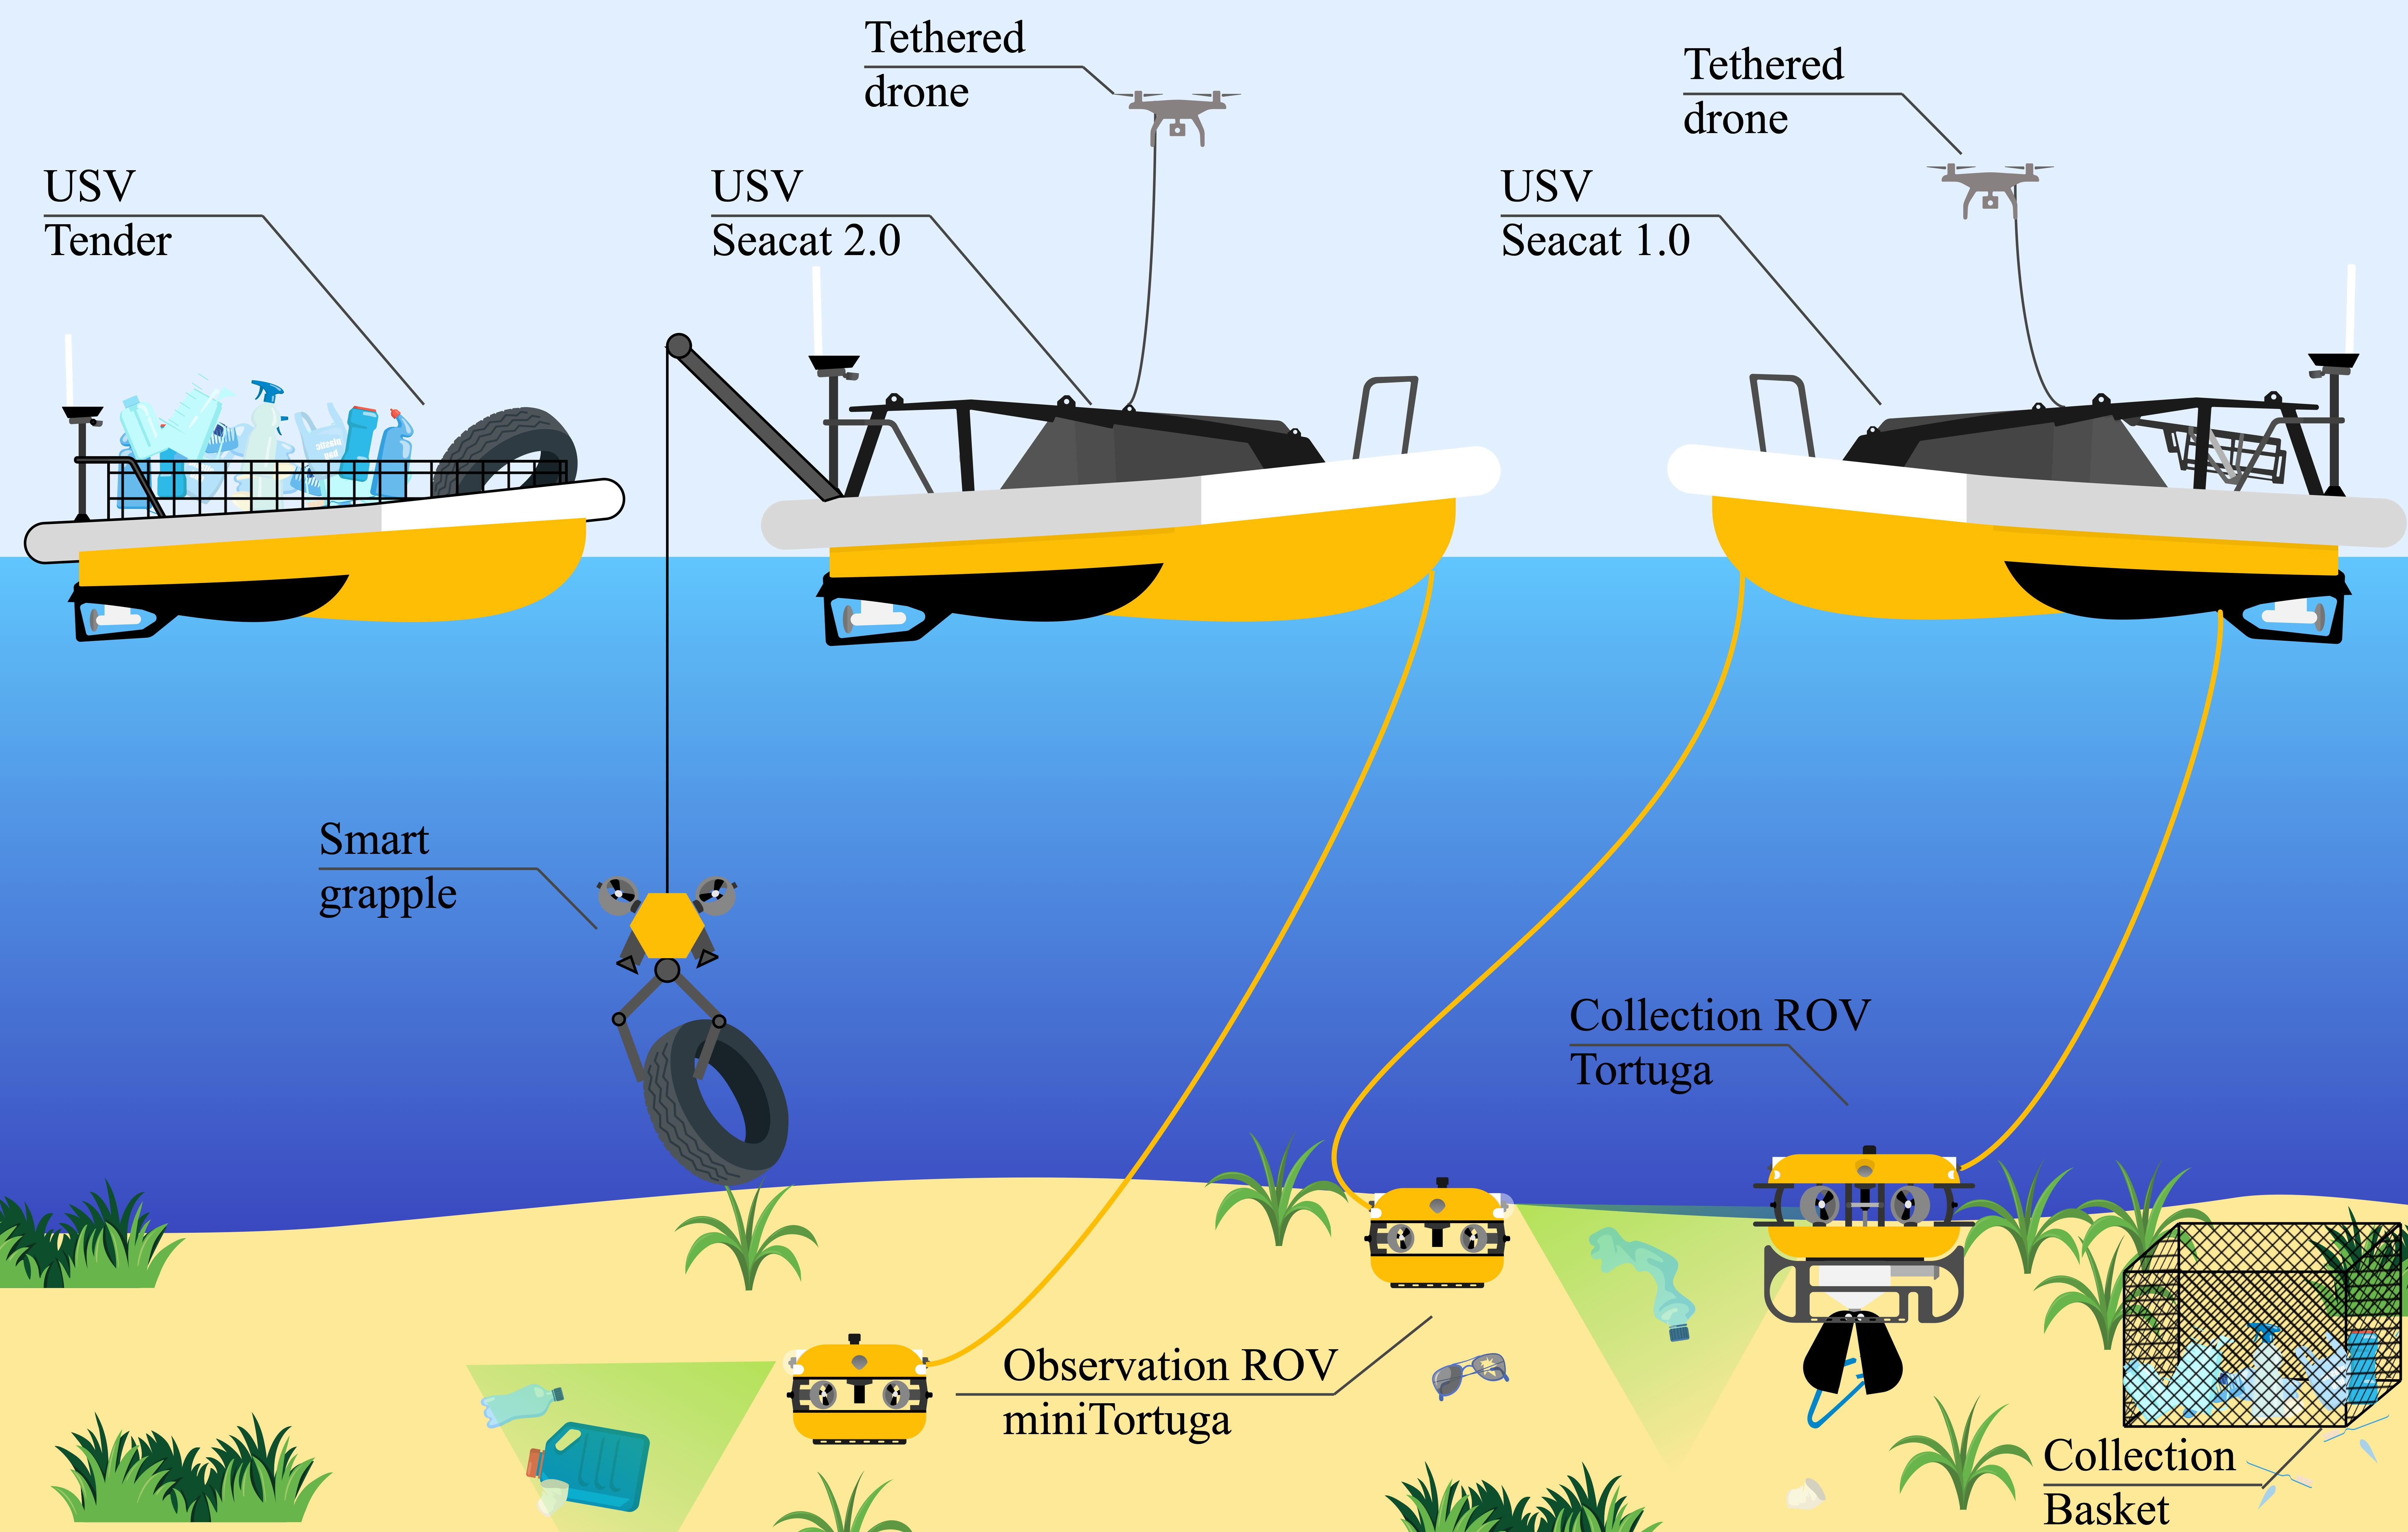
\includegraphics[width=.9\textwidth]{img/Concept_full_lowRes.jpg}
    \caption{Concept of SeaClear2.0 robotic system (left/middle) and SeaClear1.0 (right)}
    \label{fig:SC2concept }
\end{figure}

\subsection{A review of the litter collection capabilities in SeaClear1.0} \label{seaclear1_review}

In the SeaClear1.0 project the collection was limited to  small-scale and lightweight litter as a proof-of-concept, with a weight limit of up to 3 kg and a maximum size of about 30 cm. This limitation stemmed from the choice of the Tortuga robot as the robotic platform, given its maximum payload of 10 kg and overall dimensions, as well as the compatibility with the Tortuga \gls{lars} system. For the SeaClear1.0 project, this was sufficient to research the mapping and collection strategy, and focus on the predominant litter sizes at the test sites. The litter occurrence analysis in \textit{Deliverable 2.1  "Marine litter occurrence domains report"}, however, shows that there is an additional need for being able to handle both larger and heavier objects that can be found in the Mediterranean Sea and elsewhere. Furthermore, the monoocular downward-facing camera allowed for object detection and tracking, but could neither determine the distance to the object nor its 3D shape. The distance to the object was estimated from altitude measurements with the \gls{dvl}, but the quality of the measurement is highly dependent on the sound-reflecting characteristics of the seafloor at that particular spot. This triggers a demand for a redesign of the system's collection capacities in SeaClear2.0 to enhance the capabilities and robustness of the system.  


\begin{figure}
    \centering
    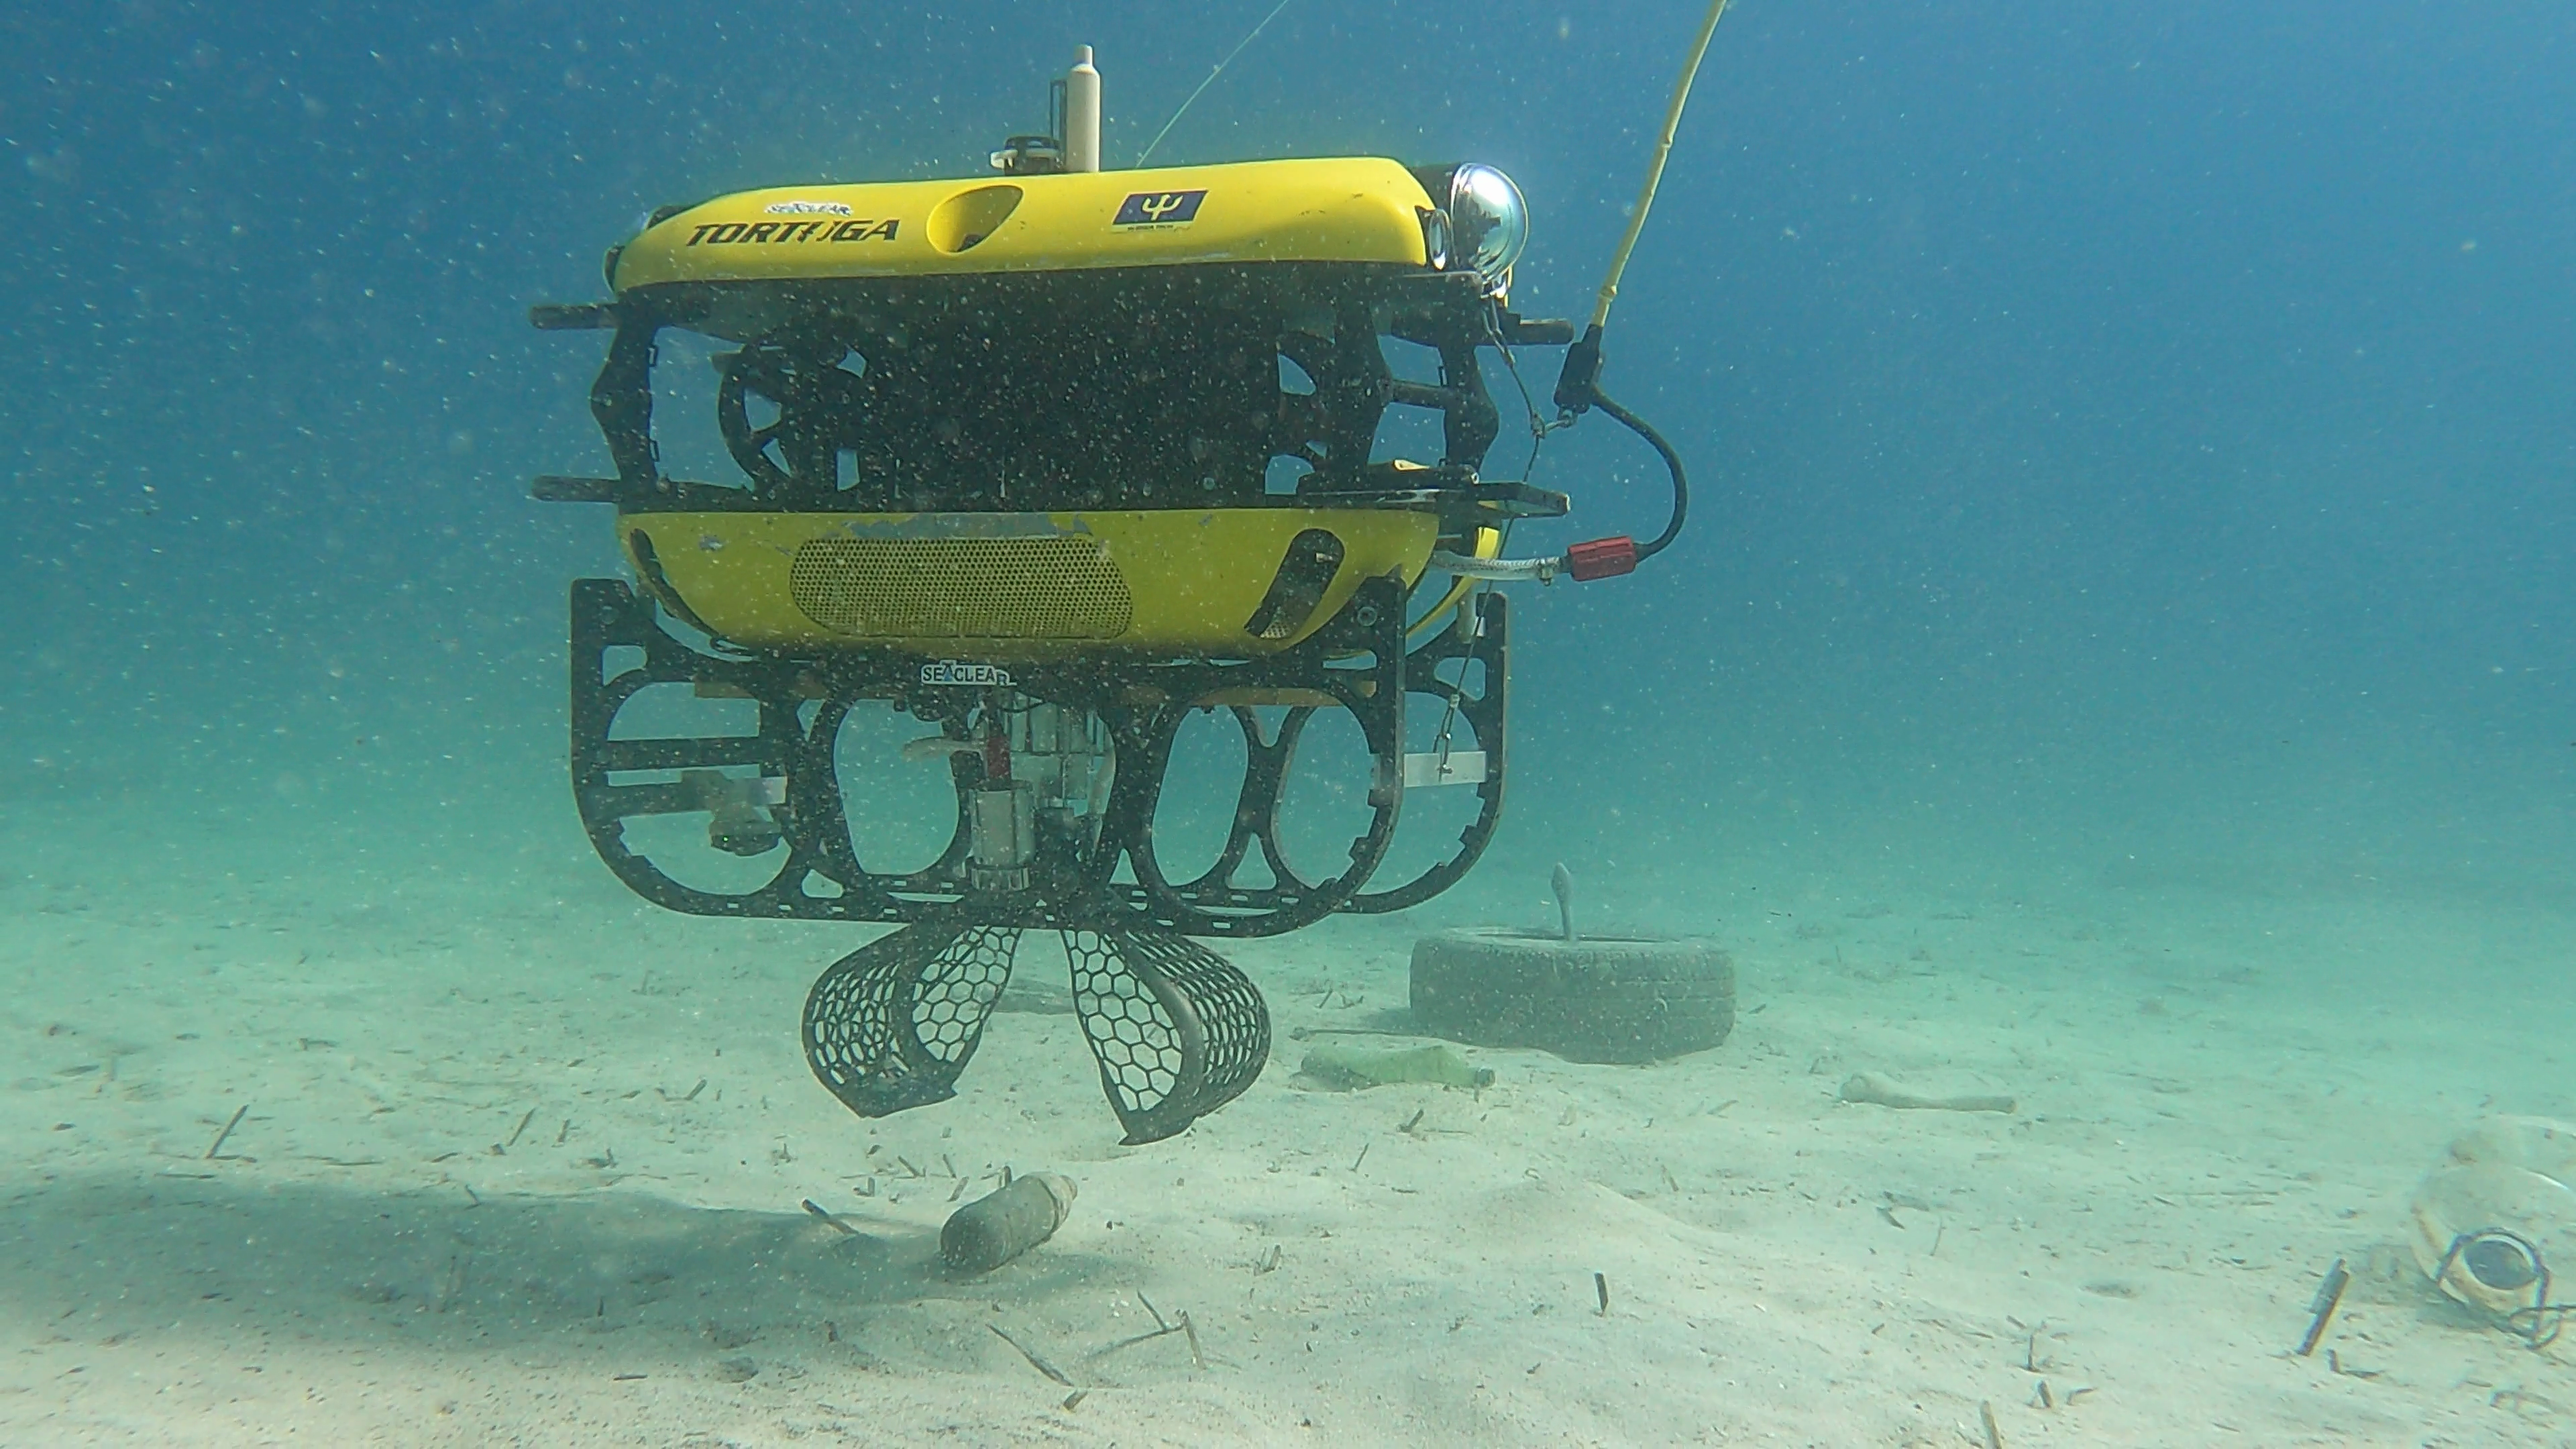
\includegraphics[width=0.6\textwidth]{img/SC1_colROV.png}
    \caption{SeaClear1.0 collection \gls{uuv} with small-scale litter.}
    \label{fig:SC1_colrov}
\end{figure}

\subsection{Deliverable objective and Document Structure}

In the SeaClear2.0 system, we focus on retrieving larger and more irregularly shaped debris, including tires, bicycles, and pipes. This represents a significant change from SeaClear1.0, as the objects are now 100 times heavier (up to 250 kg). In order to achieve collecting such items, a new smart grapple has been designed and novel capabilities developed. This activity is in direct line with objective 8 (O8): "Enhance, build and test mechanisms for efficient marine waste collection of various types of waste on different types of seafloor and on the surface" and contributes towards fulfilling the following Key Performance Indicators (KPIs):

\begin{itemize}
    \item KPI 8.1: Collect the objects from the seafloor: success rate 90\%
    \item KPI 8.2: Collect the objects from the surface: success rate 90\%
    KPI 8.3: Successful collection of various litter types: minimum 3
\end{itemize}

This deliverable documents the perception and control software framework developed for the Smart Grapple, addressing the challenges of localizing and precisely manipulating debris items under environmental disturbances. The report is structured as follows:

\begin{itemize}
    \item Section~2 describes the Smart Grapple control stack, including state estimation via sensor fusion, control allocation for the eight-thruster configuration with power constraint handling, joint control and calibration procedures, and the operational state machine governing the autonomous cycle.
    \item Section~3 presents the holistic optimal control approach for the integrated USV-USG system, covering Euler-Lagrange dynamic modeling, stochastic trajectory optimization using Risk-Aware Sample Average Approximation, and feedback augmentation for robust control under uncertainties.
    \item Section~4 details the perception system for litter localization, integrating YOLOv8-based underwater object detection with TSDF-based 3D reconstruction for metric geometry estimation.
    \item Section~5 describes the Smart Grapple grasping approach, including the torque-monitor adaptive grasping algorithm, forward and inverse kinematics solutions (analytical and FABRIK-based), optimal grasping posture analysis under joint constraints, and gripping points optimization.
    \item Section~6 presents the digital twin implementation using the MARUS simulator for software-in-the-loop testing between field deployments.
    \item Section~7 provides experimental validation through laboratory tests demonstrating 250~kg grasping capability and field results from the Marseille 2025 demonstration.
    \item Section~8 concludes with a summary of achievements and future work directions.
\end{itemize}


\section{Smart Grapple control stack}

This section describes the software architecture and control modules that enable autonomous and manual operation of the Smart Grapple system. The control stack integrates state estimation using an Extended Kalman Filter that fuses IMU and DVL sensor data for position and velocity estimation, thruster control allocation for six-degree-of-freedom maneuvering, and joint control for the eight SensoJoint actuators via EtherCAT communication within the ROS~2 framework. A hierarchical state machine orchestrates the complete operation cycle through deploying, planning, tracking, visual servoing, grasping, and recovery phases, with provisions for error handling and seamless transitions between autonomous and manual control modes through dedicated graphical user interfaces.


\subsection{Smart Grapple State Estimation}
The goal of state estimation is to compute the approximate position and velocity of the \gls{usg}. This information is required for trajectory tracking during locomotion of the robot, as described in Section~\ref{sec:trackingState}. The proposed approach leverages an \gls{ekf} on the measured sensor data to achieve state estimation.

\textbf{Sensor fusion.}
Two types of sensors are used as data sources for state estimation: an \gls{imu} and a \gls{dvl}. The \gls{imu} provides measurements of linear acceleration and angular velocity, while the \gls{dvl} provides measurements of linear and angular velocity and altitude of the vehicle relative to the seabed. In order to increase the precision of state estimation, the \gls{imu} and \gls{dvl} measurements are fused together via the \gls{ekf} \cite{10.5555/897831}.

\begin{figure}[ht]
	\centering
	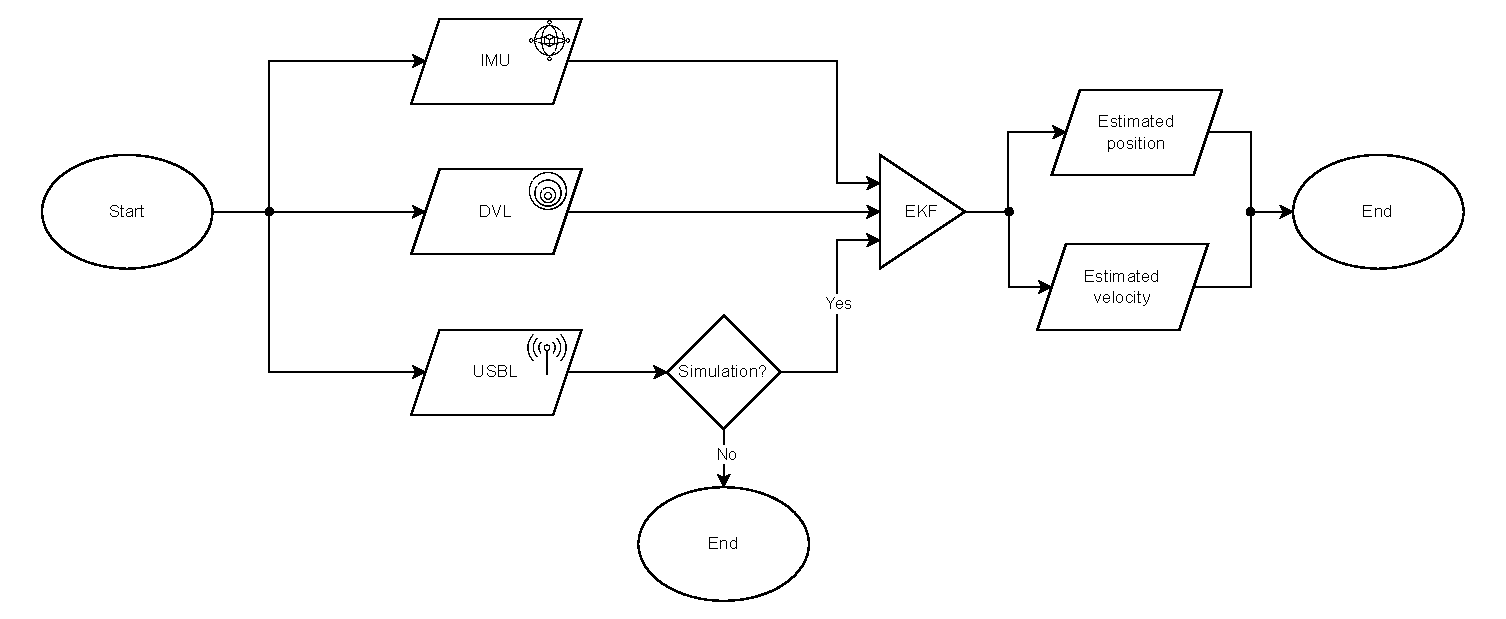
\includegraphics[width=\textwidth]{img/state_estimation_flowchart.drawio.pdf}
	\caption{Information flow of the state estimation}
	\label{fig:stateEstimationFlowchart}
\end{figure}

\textbf{Implementation.}
The \textit{robot\_localization} package, developed by Charles River Analytics, is used to implement the \gls{ekf} \cite{MooreStouchKeneralizedEkf2014}. It is an open-source package that provides a basic framework for localization tasks that can be easily adapted to different robotic systems such as the \gls{usg}. The main benefits of this package are:
\begin{itemize}
    \item Supports ROS 2 out-of-the-box,
    \item Handles an unlimited number of inputs from multiple sensor types,
    \item Allows 3D localization,
    \item Provides higher control over the sensor data and how it impacts the estimation.
\end{itemize}

\textbf{Simulation.}
The state estimation module is part of the digital twin. The data sources for sensor fusion in simulation are slightly different as they also include \gls{gnss} measurements. These measurements are used to emulate a \gls{usbl} acoustic positioning system, which will be added to the \gls{usg} hardware in the future. For more details on the digital twin, refer to Section~\ref{sec:sim}.

\subsection{Smart Grapple Control Allocation}

This section describes the control allocation system that distributes commanded wrenches across the eight thrusters mounted on the \gls{usg}. The allocation matrix is derived from the geometric configuration of the thrusters, mapping individual thrust commands to the resulting six-degree-of-freedom wrench at the center of mass. To handle the 5~kW power constraint shared among all thrusters, a quadratic programming formulation with a percentage phase-back post-processing strategy is employed, which maintains real-time computational feasibility (average runtime of 18~ms) while achieving tracking performance within 15.6\% of the optimal nonlinear solution.


\subsubsection{Thruster Positions on the Hardware}

\begin{figure}[!h]
    \centering
    %----------------------------------------------------------
    \begin{subfigure}[t]{0.48\textwidth}
        \centering
        % Crop left, bottom, right, top (adjust as needed)
        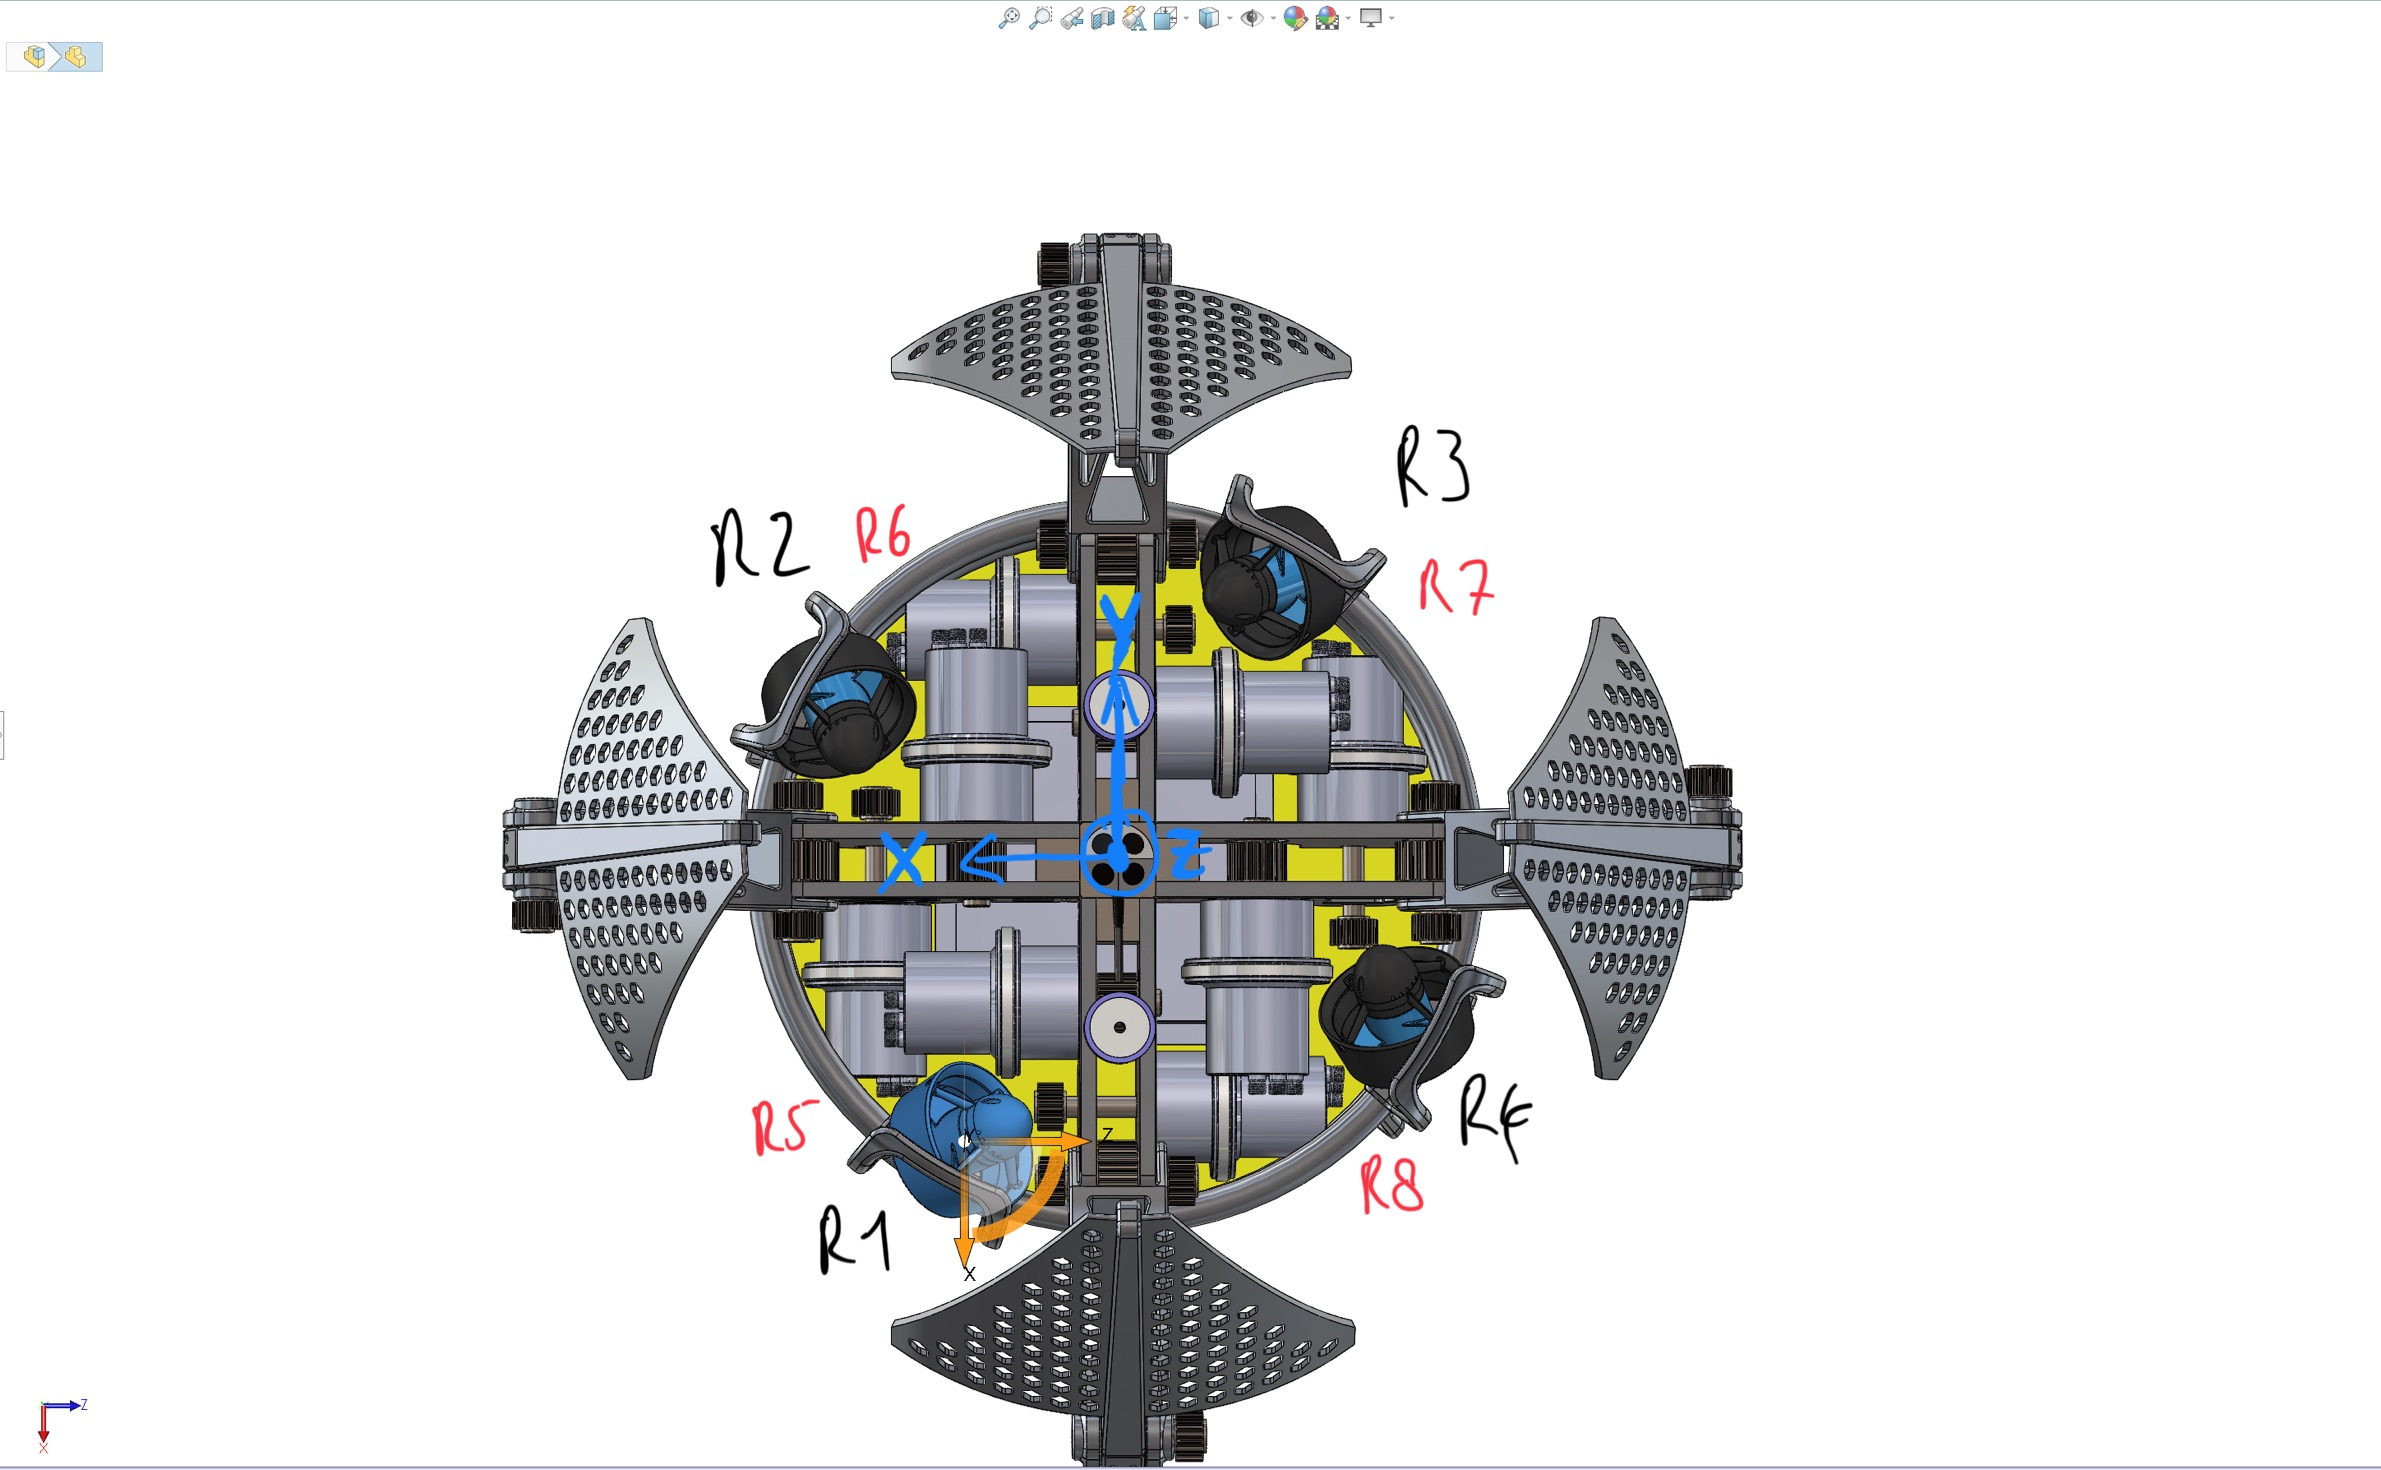
\includegraphics[width=\textwidth, trim={4cm 2cm 4cm 4cm}, clip]{img/bottom_view_thrusters.jpeg}
        \caption{Bottom view (looking along $-\!Z_{\mathrm{ref}}$). Thrusters R1–R4 shown in \textcolor{black}{black} (visible) and occluded units in \textcolor{red}{red}.}
        \label{fig:thrusters_bottom}
    \end{subfigure}
    \hfill
    %----------------------------------------------------------
    \begin{subfigure}[t]{0.48\textwidth}
        \centering
        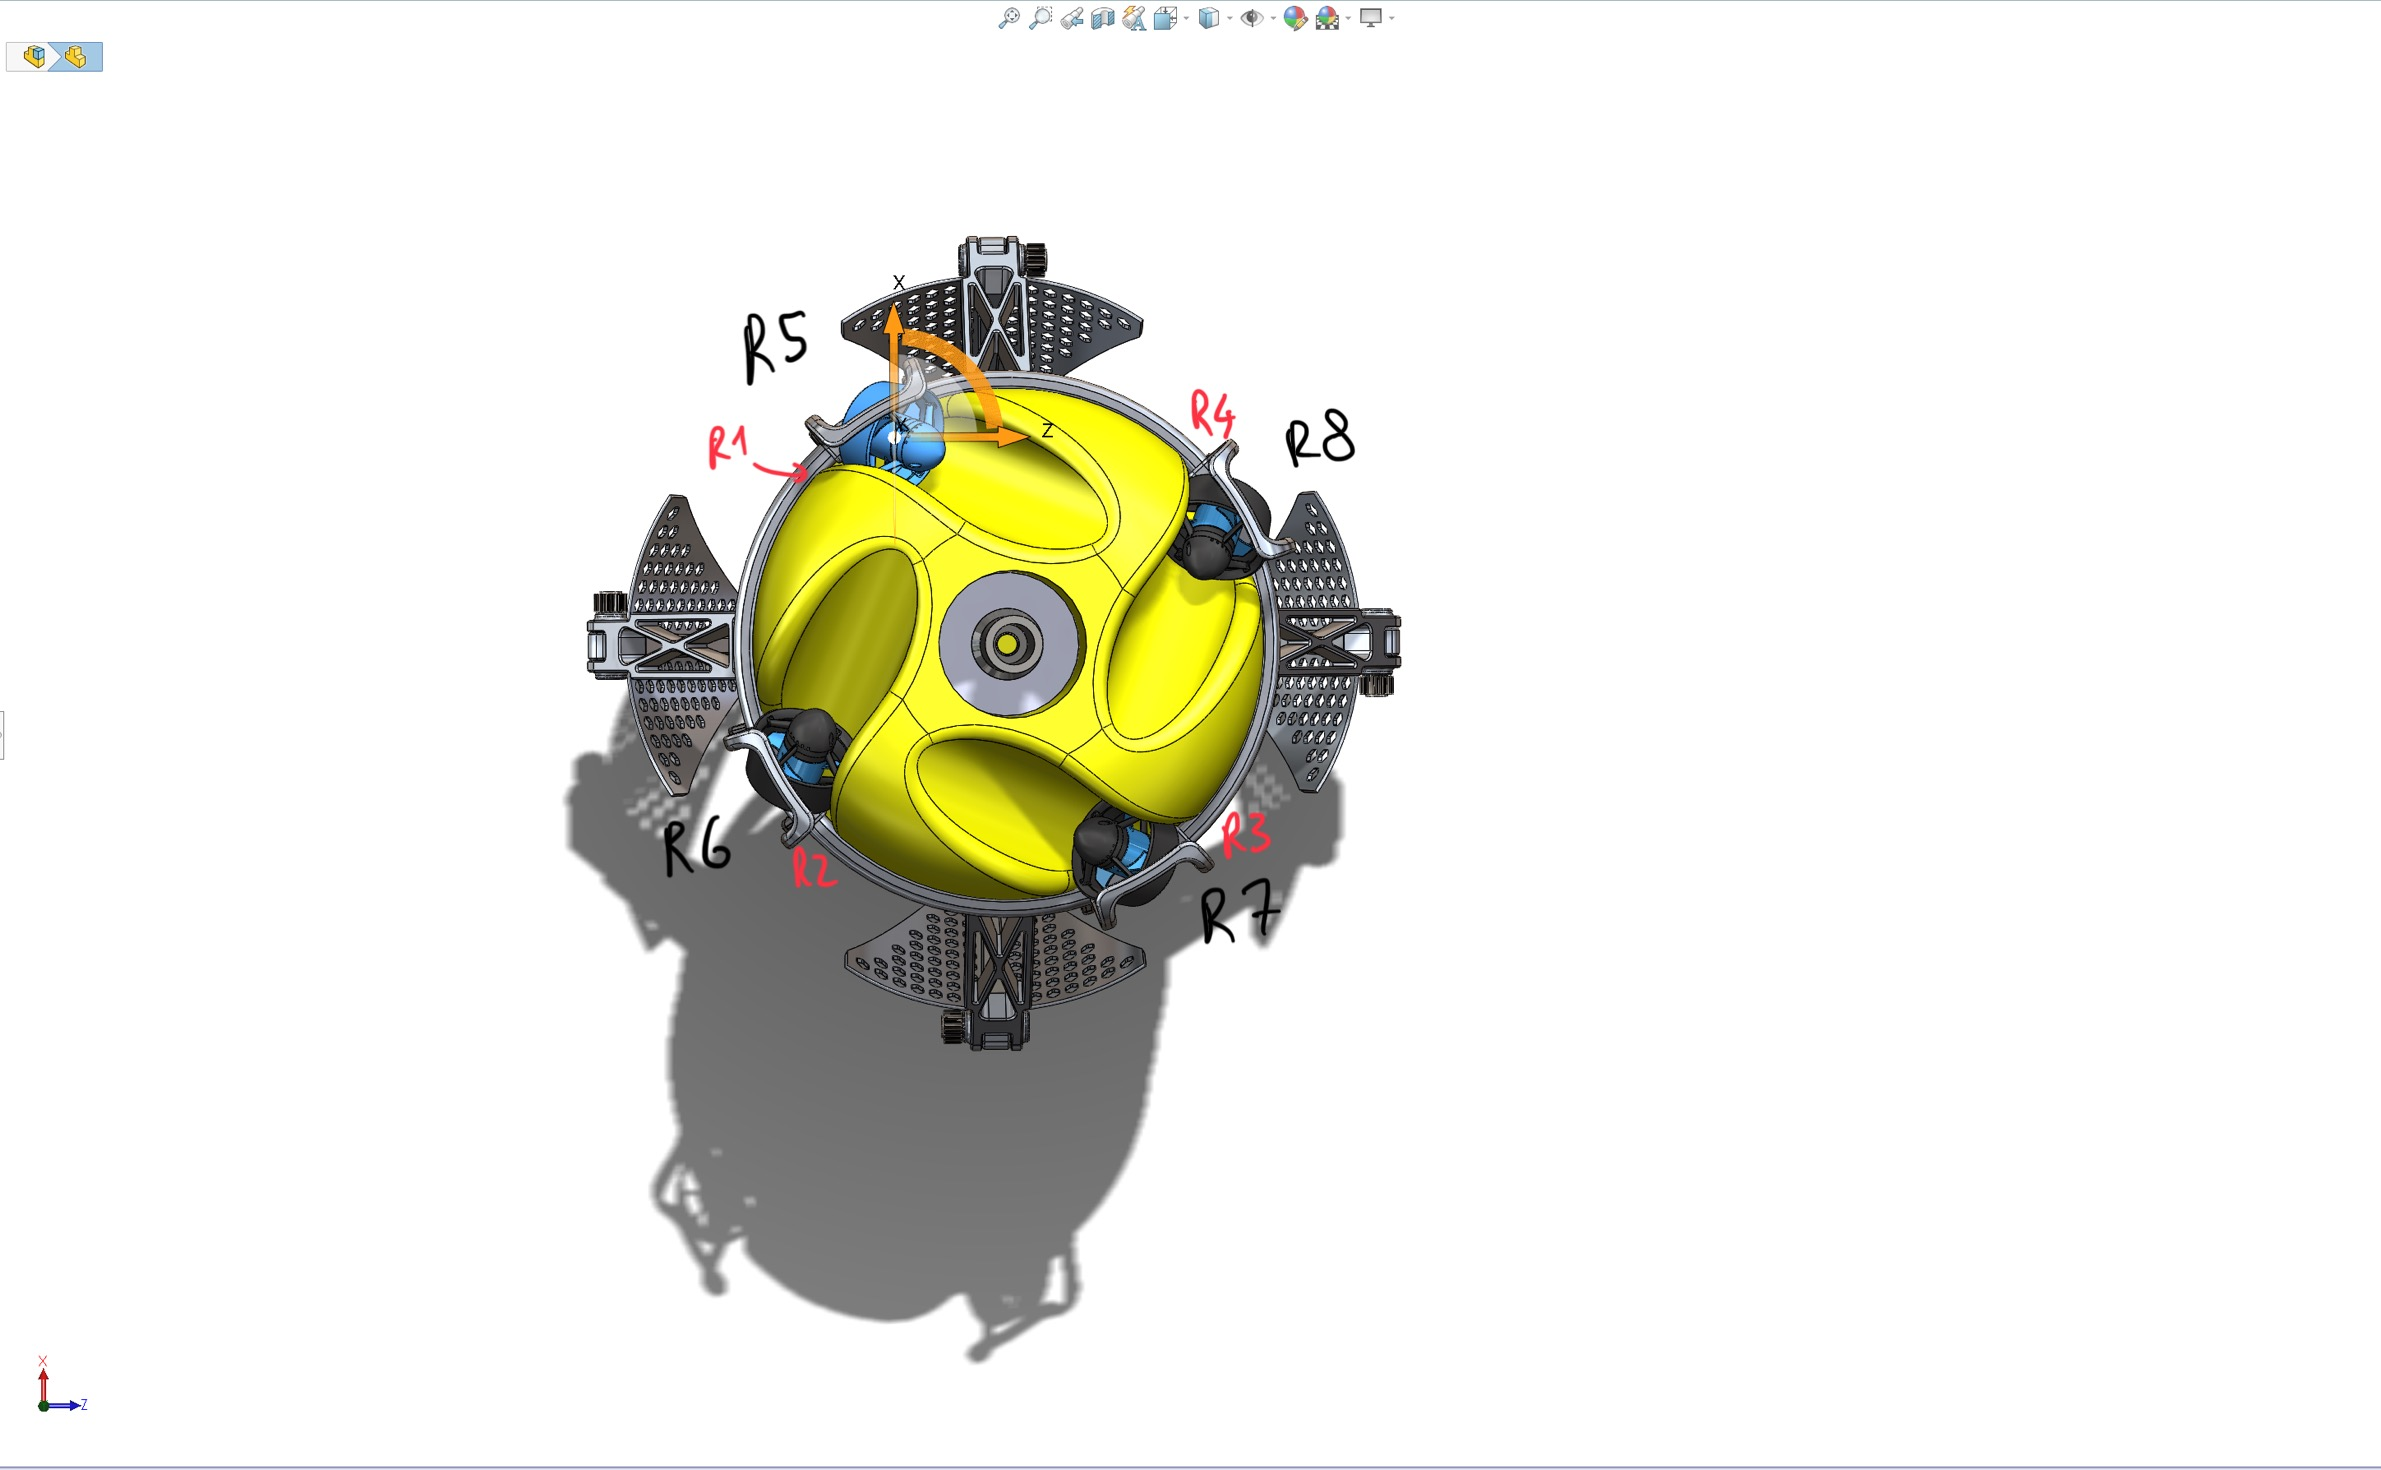
\includegraphics[width=\textwidth, trim={15cm 14cm 15cm 8cm}, clip]{img/top_view_thrusters.jpeg}
        \caption{Top view (looking along $+\!Z_{\mathrm{ref}}$). Thrusters R5–R8 shown in \textcolor{black}{black} (visible) and occluded units in \textcolor{red}{red}.}
        \label{fig:thrusters_top}
    \end{subfigure}
    %----------------------------------------------------------
    \caption{Thruster layout of the \gls{usg} platform in the reference frame $\mathcal{F}_{\mathrm{ref}}$ \textcolor{blue}{blue} \ian{in (a)}.
    \bds{It is not clear to me what "blue" refers to here}
    Subfigure~\subref{fig:thrusters_bottom} depicts the bottom assembly (R1–R4), and Subfigure~\subref{fig:thrusters_top} the top assembly (R5–R8).
    Color coding: \textcolor{black}{black} = visible in the current viewpoint; \textcolor{red}{red} = occluded.}
    \label{fig:thruster_overview}
\end{figure}
\begin{figure}[h!]
    \centering
    % Five rotated images with minimal whitespace
    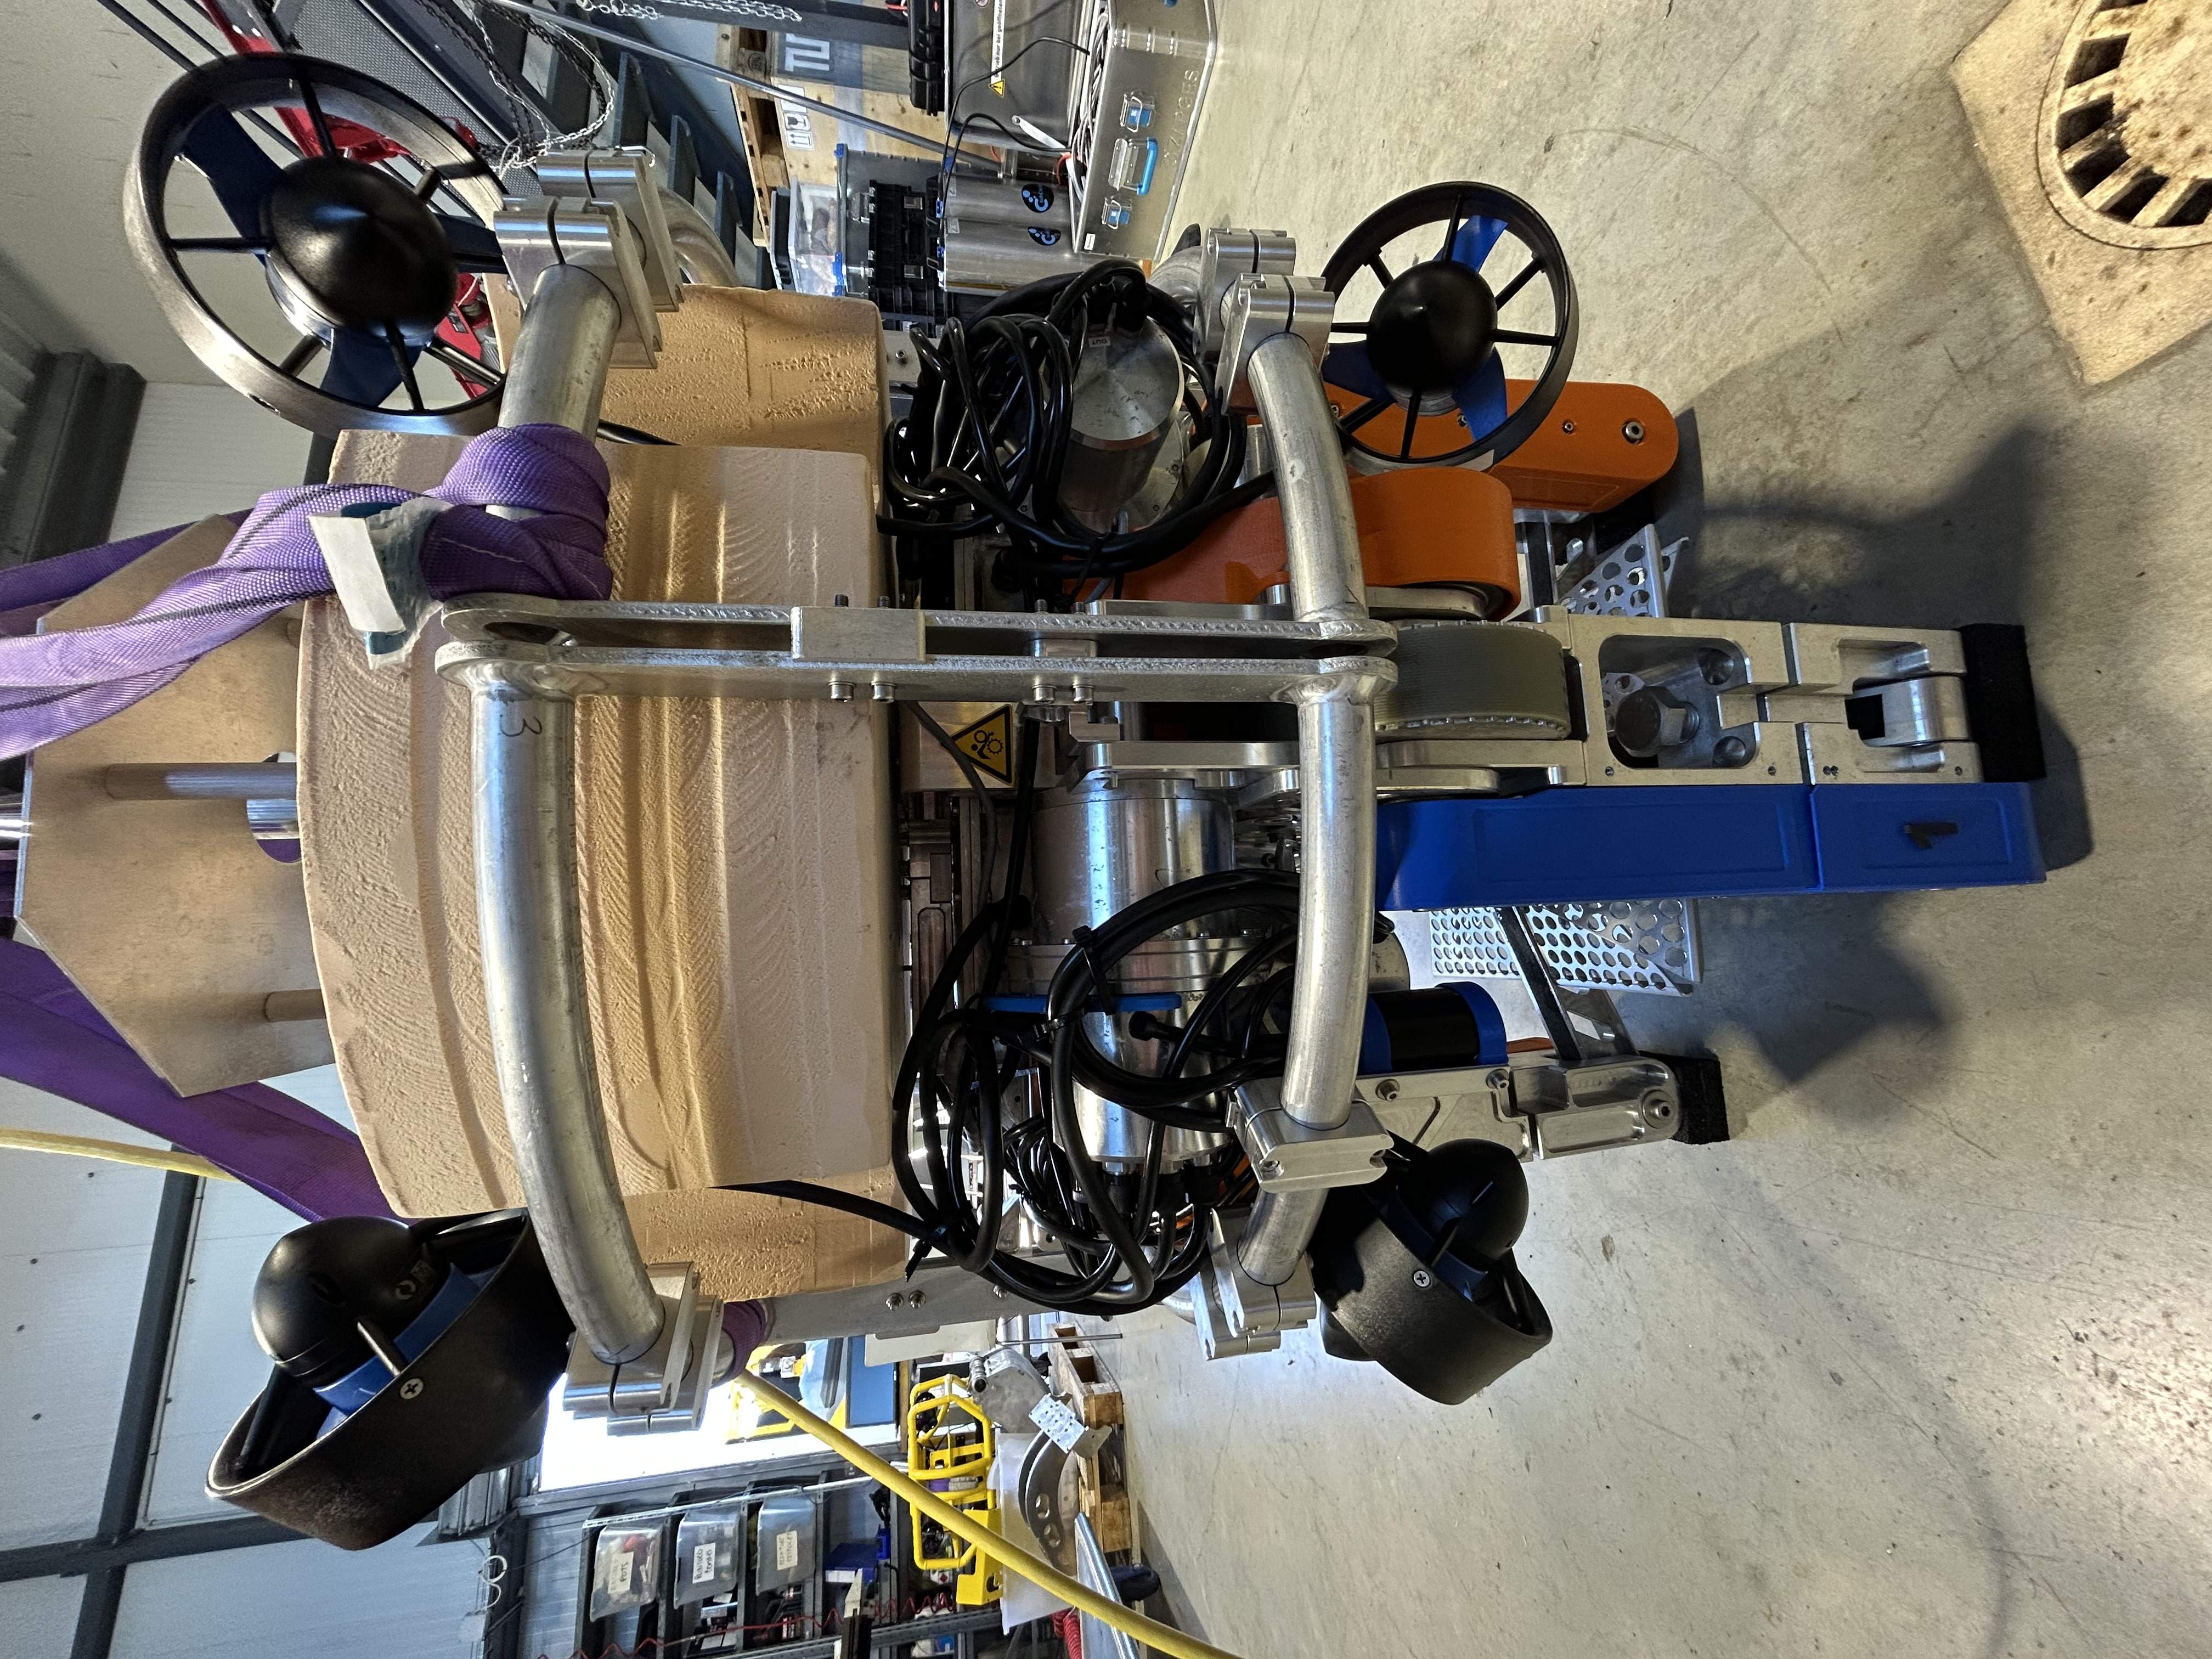
\includegraphics[width=0.25\textwidth, angle=270, origin=c]{img/grapple_thrusters_1.jpeg}\hspace{2pt}%
    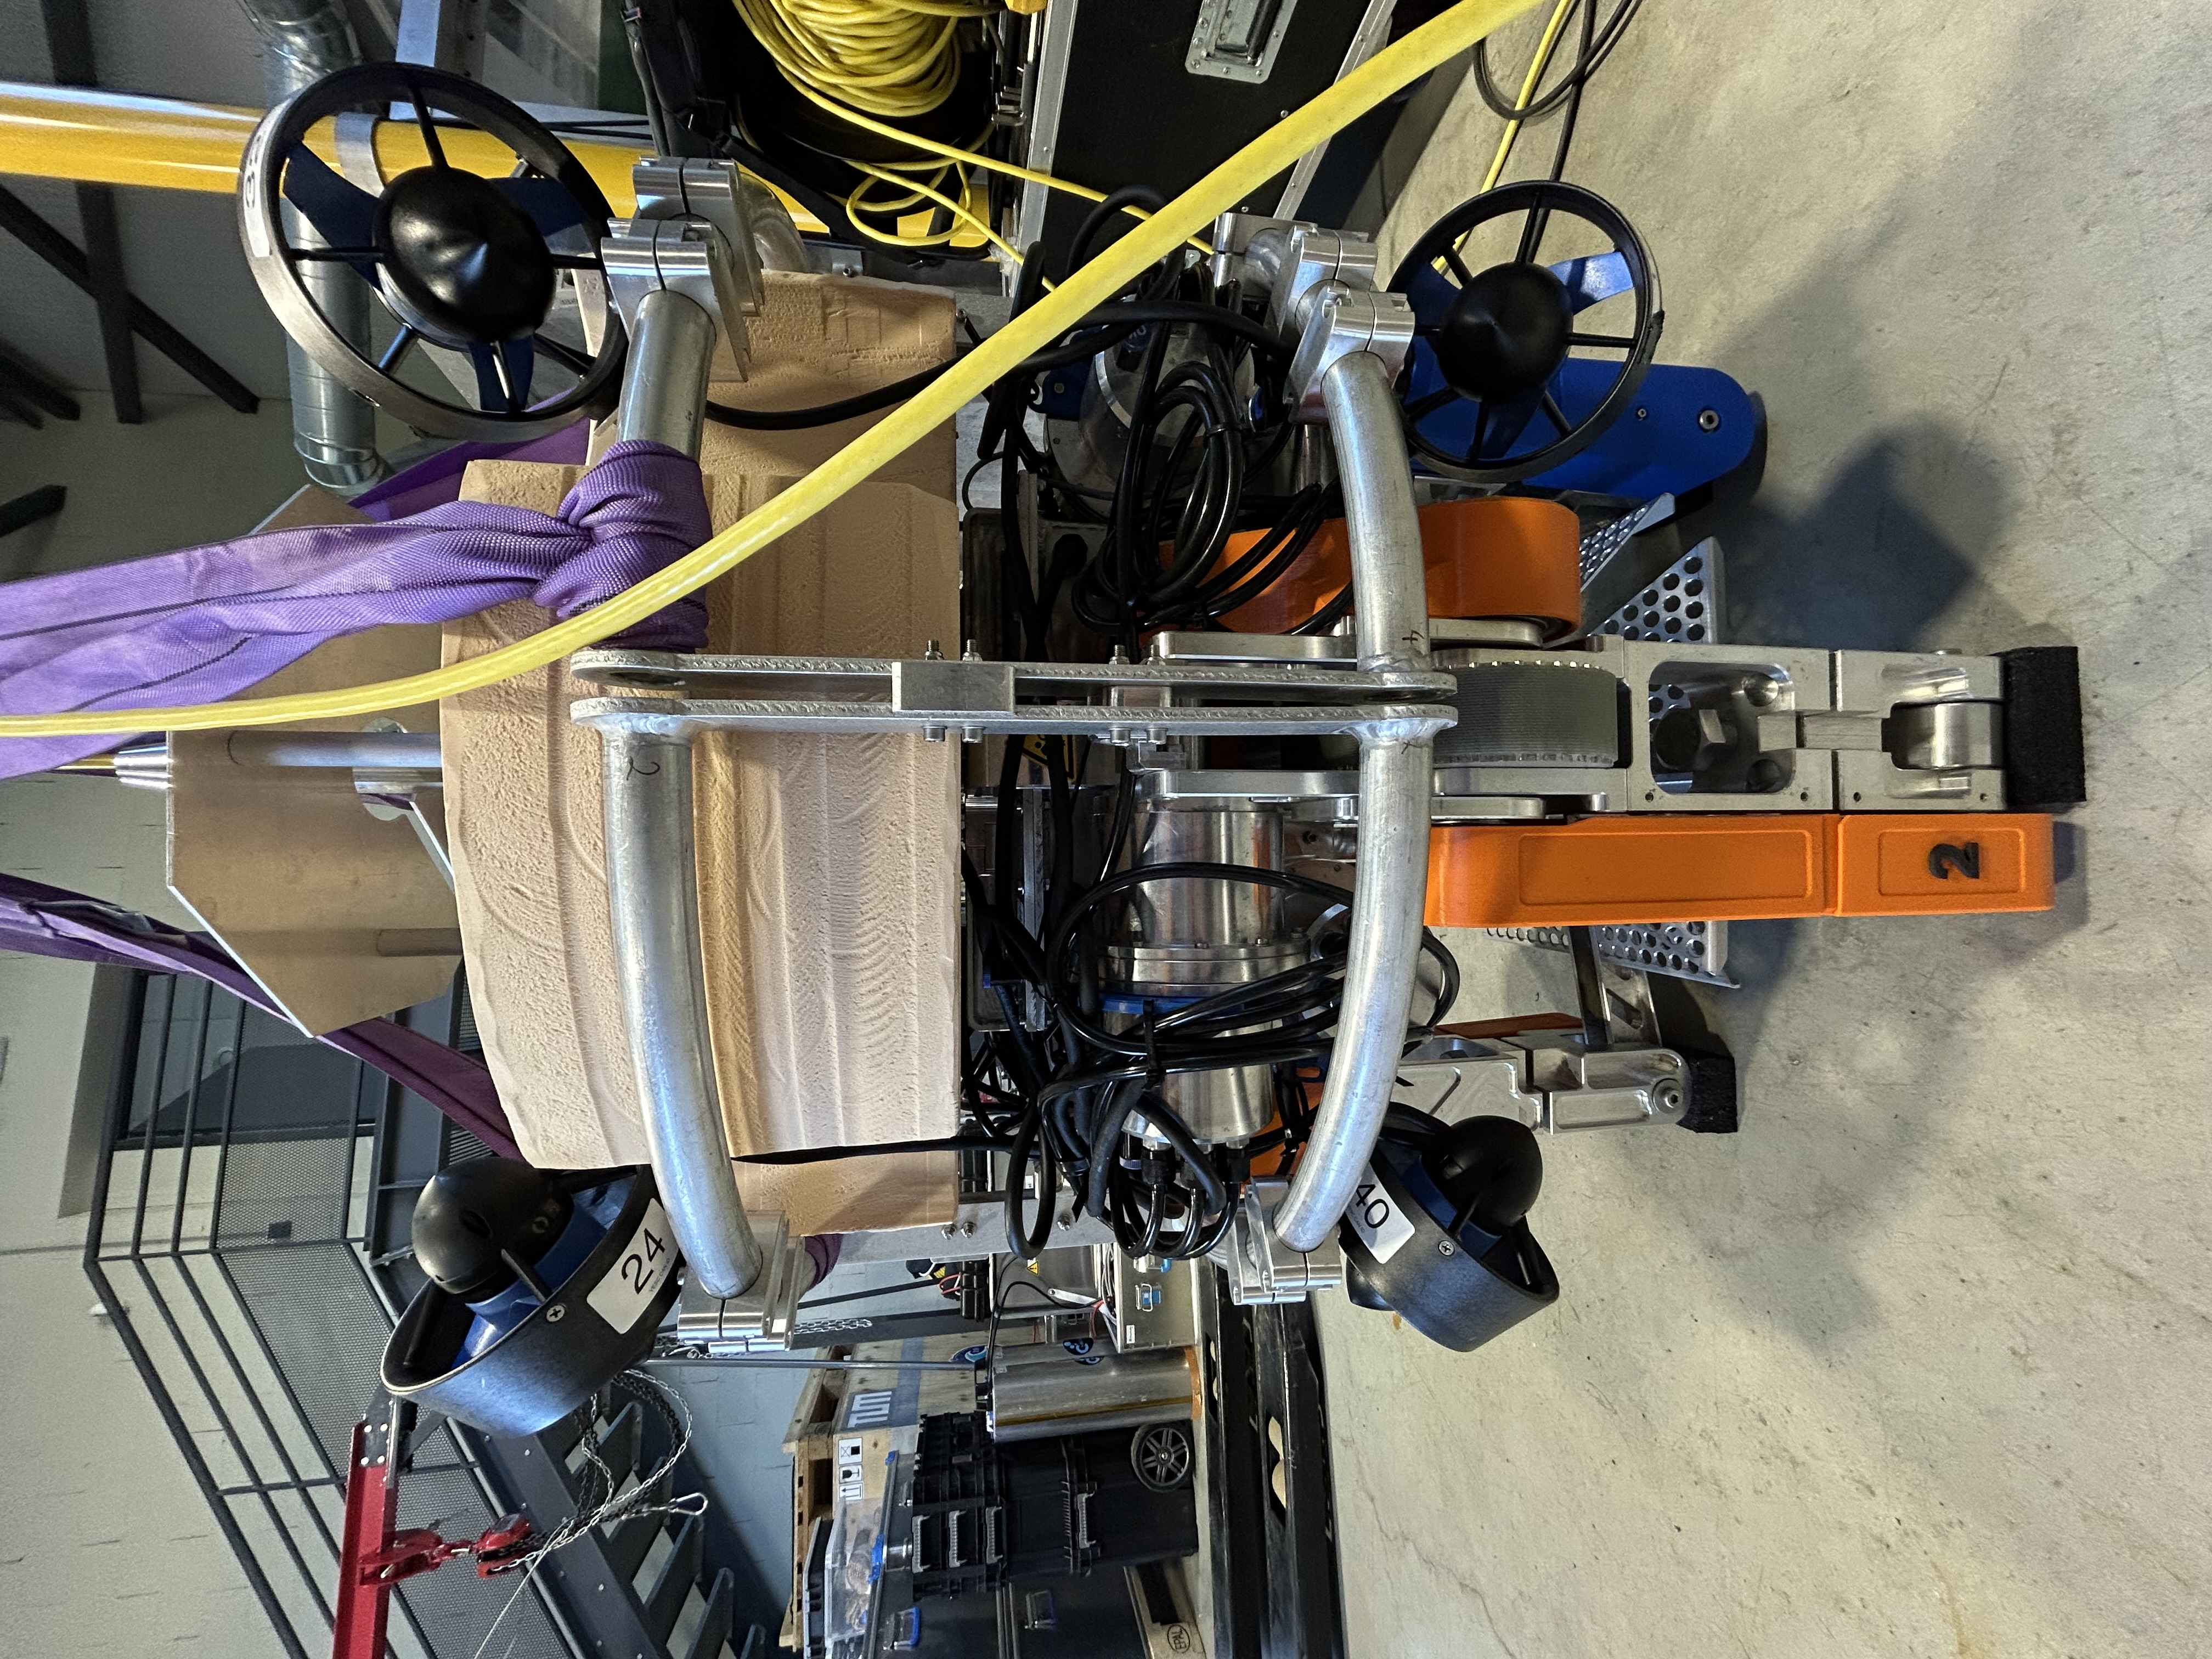
\includegraphics[width=0.25\textwidth, angle=270, origin=c]{img/grapple_thrusters_2.jpeg}\hspace{2pt}%
    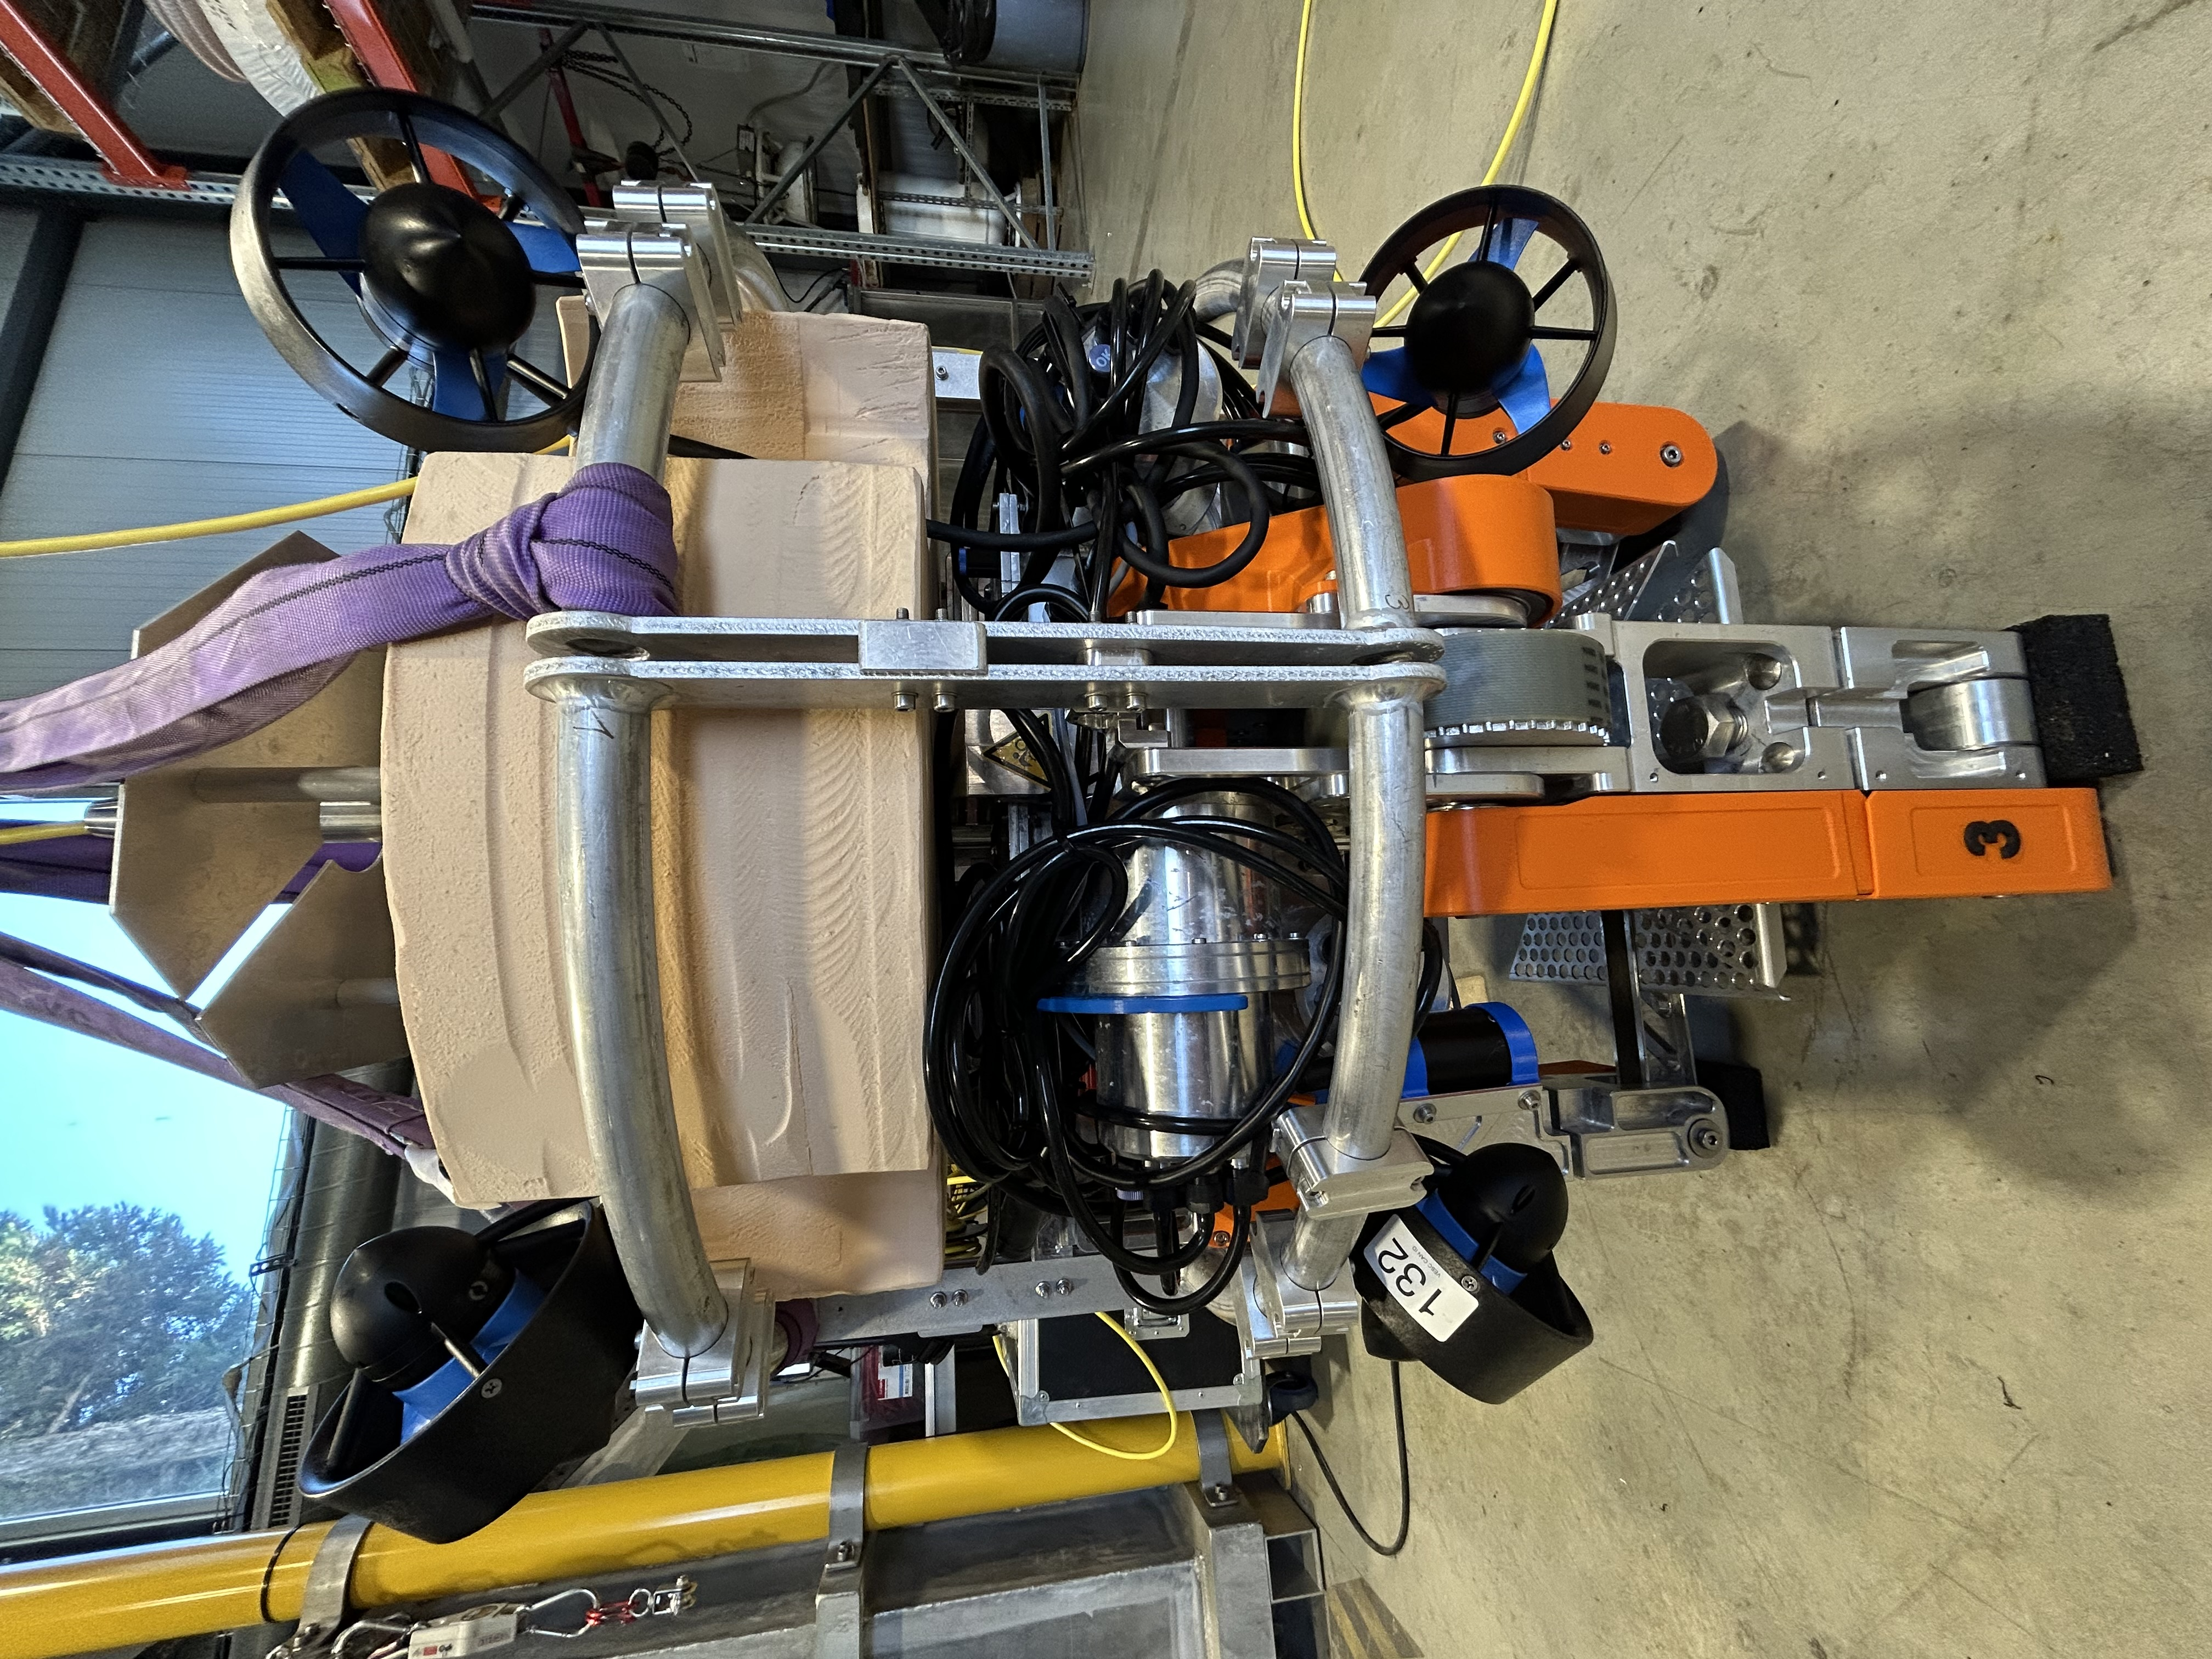
\includegraphics[width=0.25\textwidth, angle=270, origin=c]{img/grapple_thrusters_3.jpeg}\hspace{2pt}%
    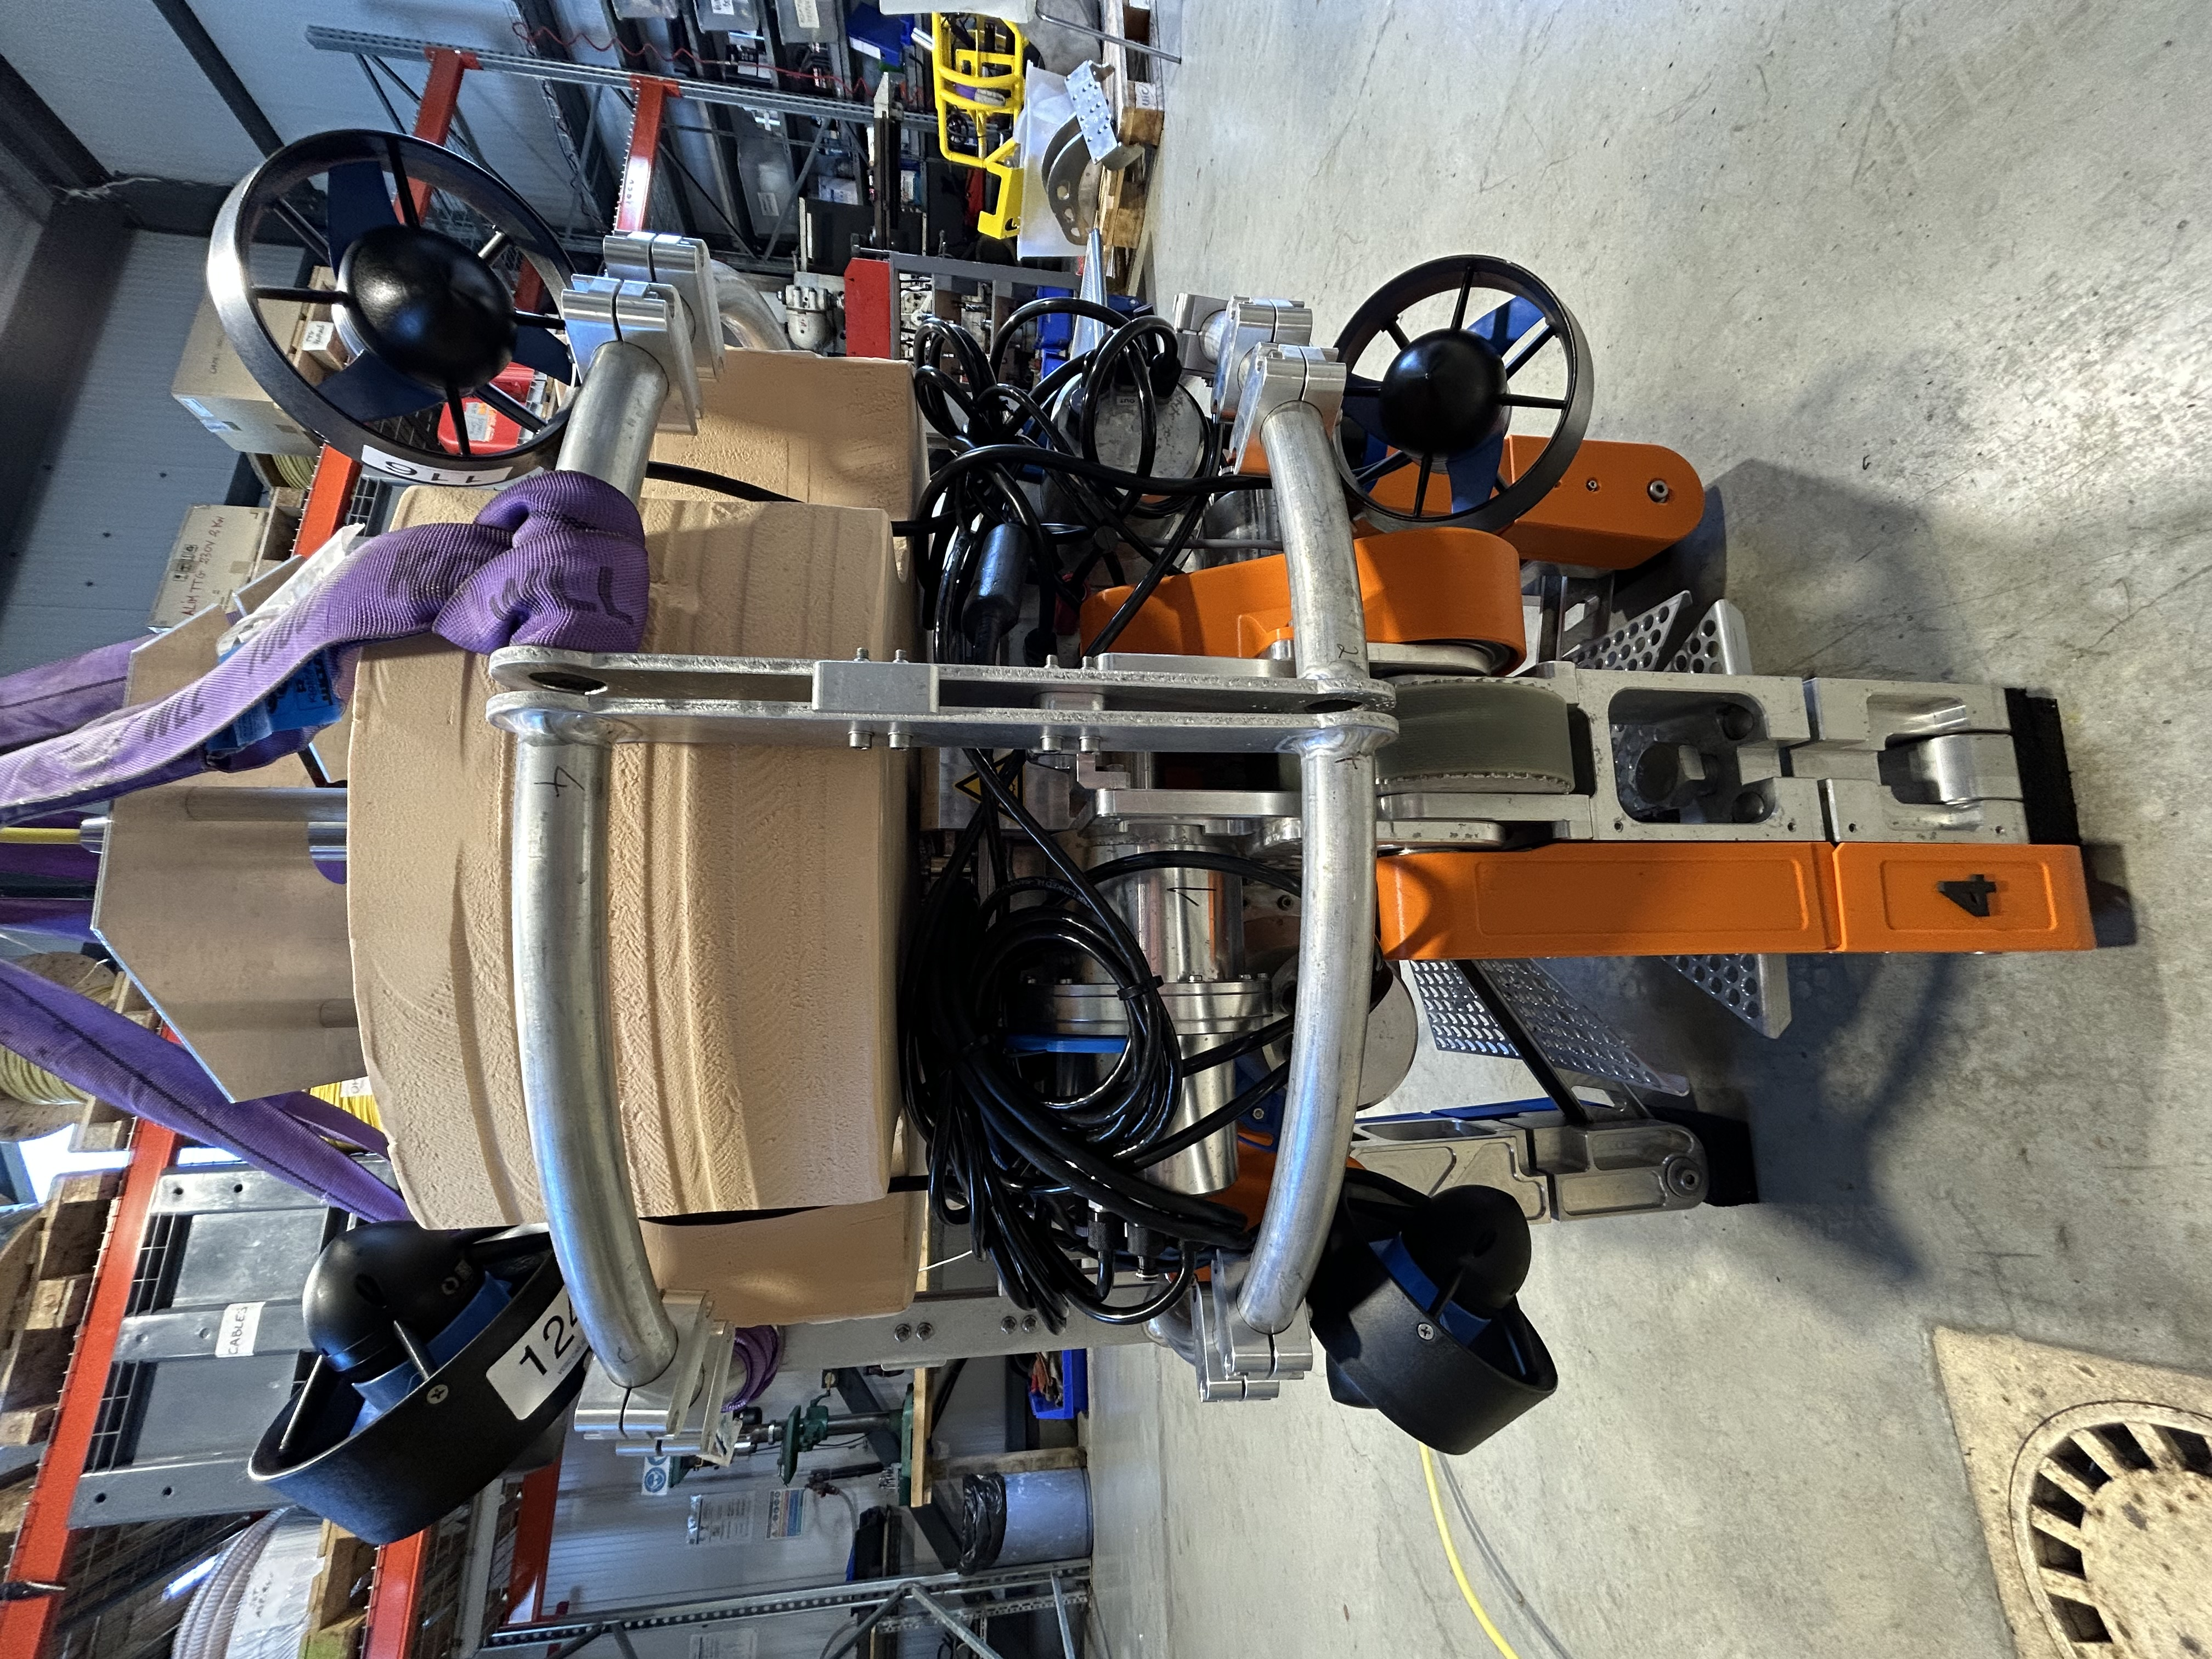
\includegraphics[width=0.25\textwidth, angle=270, origin=c]{img/grapple_thrusters_4.jpeg}\hspace{2pt}%
    \caption{Thrusters layout on the hardware: Marseille (September 2025).}
    \label{fig:thrursters_layout}
\end{figure}

A detailed table on the positions and orientations of the thrusters can be found in Appendix~\ref{appendix:thrustalloc}.


\subsubsection{Derivation of the Control Allocation Matrix}

\bds{Later on 8 is directly used in stead of the general $N$ as on the next line - maybe best link explicitly}
Each thruster \ian{$i \in \{1,\dots,8\}$} is rigidly mounted on the \gls{usg} and defined by its pose with respect to the \gls{usg} reference frame
$\mathcal{F}_{\mathrm{ref}} = (X_{\mathrm{ref}}, Y_{\mathrm{ref}}, Z_{\mathrm{ref}})$.
\paragraph{Position}
Let $\vec{p}_i \in \mathbb{R}^3$ denote the nominal mounting position of thruster $i$ 
expressed in the reference frame $\mathcal{F}_{\mathrm{ref}}$.
Since the allocation matrix is referenced to the \gls{usg}'s \gls{com}, 
located at $\vec{r}_{\mathrm{COM}} = [0, \, 0, \, 0.1362]^\top $, the position vector of thruster $i$ relative to the COM becomes
\begin{align}
\vec{r}_i = R_z(\alpha_0)\,(\vec{p}_i - \vec{r}_{\mathrm{COM}}),
\qquad \alpha_0 = -9^\circ.
\end{align}
because the positions in Table \ref{tab:thruster_pose_nominal_vesc} are expressed \textbf{without }the shift around $Z_{\mathrm{ref}}$ of $\alpha_0 = -9^\circ$, which is seen on Figure \ref{fig:thruster_overview} and in the hardware Figure~\ref{fig:thrursters_layout}. Note that the \gls{com} serves as the reference point for the wrench computation.

\subsection*{Orientation}
Each thruster orientation is defined by the angles
$(\theta_i^{(y)}, \theta_i^{(z)}, \theta_i^{(x)}, \psi_i^{(z)})$.
With
\begin{align}
R_x(\alpha)&=\begin{bmatrix}1&0&0\\0&\cos\alpha&-\sin\alpha\\0&\sin\alpha&\cos\alpha\end{bmatrix}, &
R_y(\alpha)&=\begin{bmatrix}\cos\alpha&0&\sin\alpha\\0&1&0\\-\sin\alpha&0&\cos\alpha\end{bmatrix}, &
R_z(\alpha)&=\begin{bmatrix}\cos\alpha&-\sin\alpha&0\\\sin\alpha&\cos\alpha&0\\0&0&1\end{bmatrix},
\end{align}
the rotation from $\mathcal{F}_i$ to $\mathcal{F}_{\mathrm{ref}}$ is
\begin{align}
R_i = R_z\!\bigl(\psi_i^{(z)}\bigr)
       \bigl(R_x(\theta_i^{(x)})\,R_z(\theta_i^{(z)})\,R_y(\theta_i^{(y)})\bigr).
\end{align}
The inner product of matrices in parentheses represents three consecutive intrinsic rotations, applied successively about the current $y$, $z$, $x$-axes of the thruster. The leading factor $R_z\!\bigl(\psi_i^{(z)}\bigr)$ introduces an additional extrinsic rotation about the fixed $Z_{\mathrm{ref}}$-axis, which represents the shift of $90^\circ$ between consecutive thrusters (Table \ref{tab:thruster_pose_nominal_vesc}).

\paragraph{Homogeneous Transformation} \ian{The transformation matrix with translation and rotation:}
\bds{Best add a sentence or phrase here to aboid a floating equation and to explain what this is}
\begin{align}
{}^{\mathrm{ref}}T_i =
\begin{bmatrix}
R_i & \vec{r}_i\\
\vec{0}^\top & 1
\end{bmatrix}.
\end{align}

\paragraph{Force and Moment Mapping}
Each thruster produces a thrust $u_i$ along its local $+Z_i$-axis:
\begin{align}
\vec{f}_i^{(i)} &= \begin{bmatrix}0\\0\\t_i\end{bmatrix}, &
\vec{f}_i &= R_i\,\vec{f}_i^{(i)} = u_i\,\vec{a}_i,
\quad
\vec{a}_i \coloneqq R_i\!\begin{bmatrix}0\\0\\1\end{bmatrix}.
\end{align}
The resulting moment about the \gls{com} is
\begin{align}
\vec{m}_i = \vec{r}_i \times \vec{f}_i
             = u_i\,(\vec{r}_i \times \vec{a}_i).
\end{align}
The corresponding wrench is
\begin{align}
\vec{\tau}_i =
u_i
\begin{bmatrix}
\vec{a}_i\\
\vec{r}_i \times \vec{a}_i
\end{bmatrix}.
\end{align}
\paragraph{Allocation Matrix}
Stacking all $8$ thrusters gives
\begin{align}
\Mat{B} =
\begin{bmatrix}
\vec{a}_1 & \cdots & \vec{a}_8\\
\vec{r}_1 \times \vec{a}_1 & \cdots & \vec{r}_8 \times \vec{a}_8
\end{bmatrix} \in \mathbb{R}^{6\times 8}, \qquad
\vec{u} = [u_1,\dots,u_8]^\top,
\end{align}
such that
\begin{align}
\boxed{
\vec{\tau} =
\begin{bmatrix}\vec{F}\\\vec{M}\end{bmatrix}
= \Mat{B}\,\vec{u}.
}
\end{align}
\begin{figure}[h!]
    \centering

    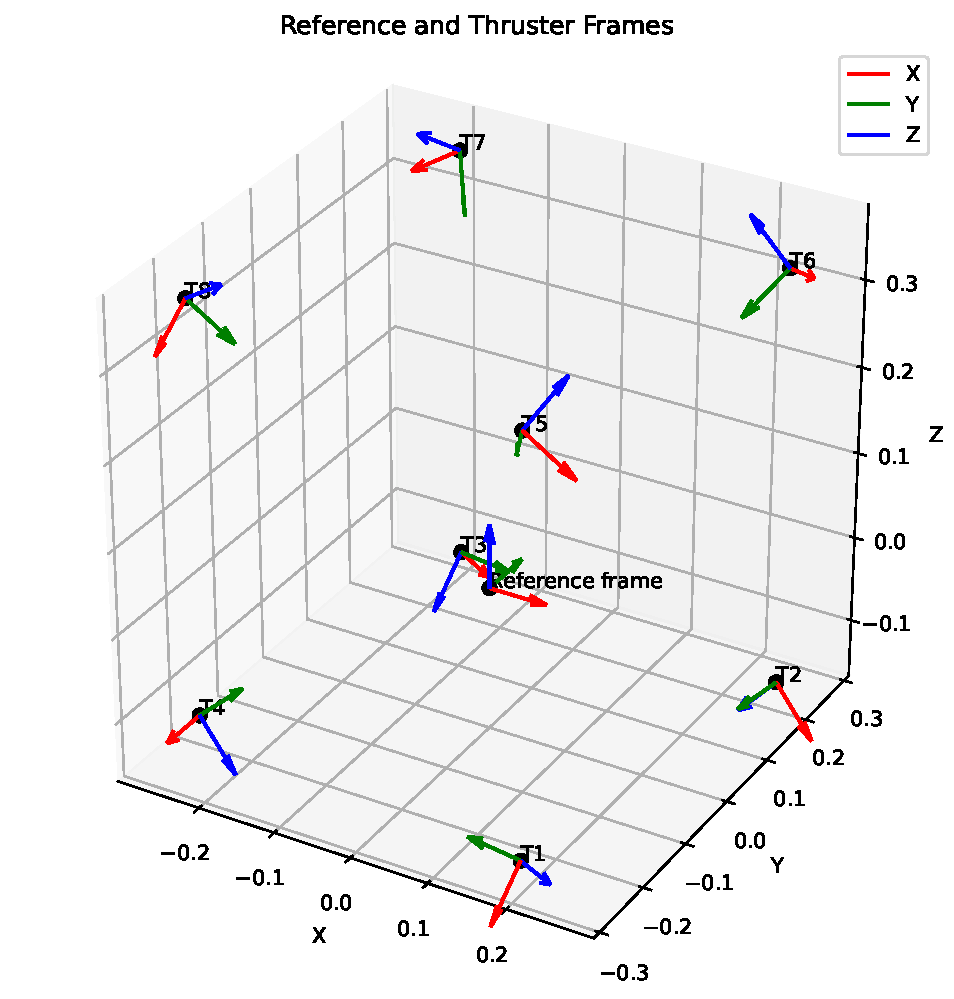
\includegraphics[width=0.28\textwidth, trim={1.5cm 0cm 0cm 0.9cm}, clip]{img/thruster_frames_1.pdf}\hspace{0pt}%
    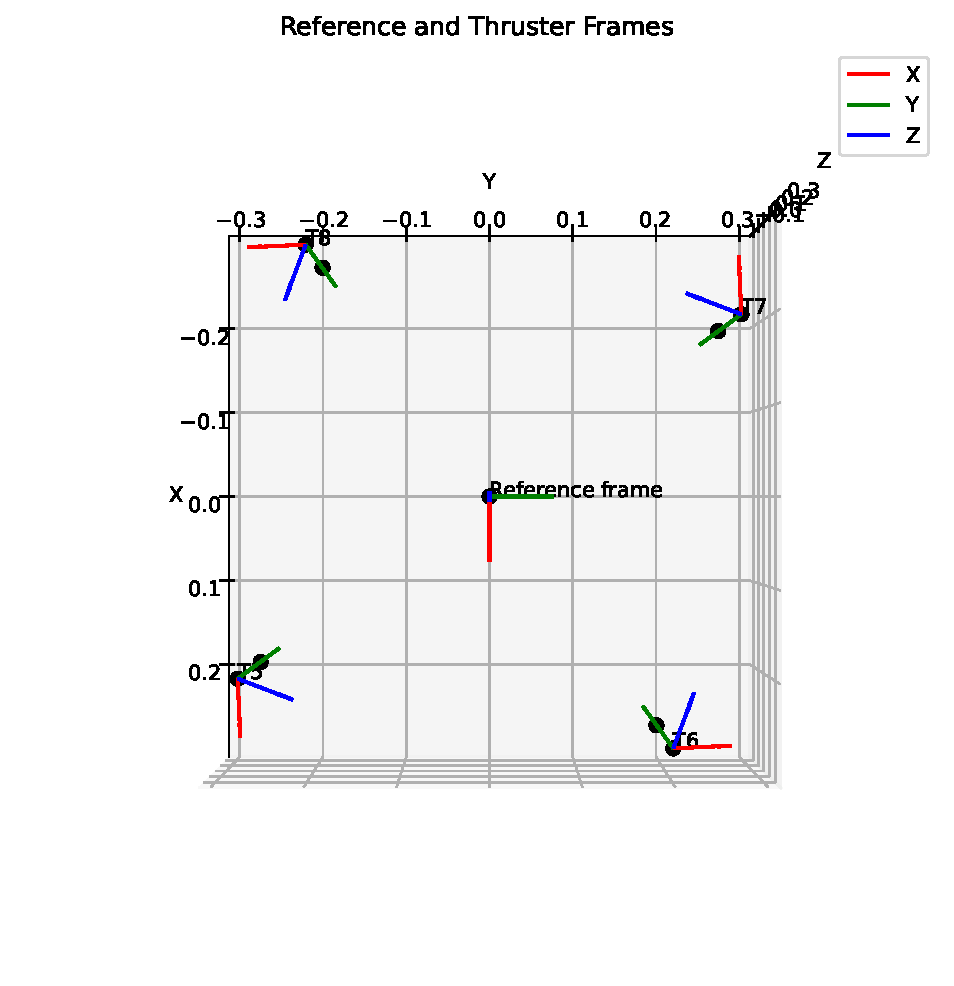
\includegraphics[width=0.37\textwidth, trim={1.5cm 1cm 0cm 0.9cm}, clip]{img/thruster_frames_2.pdf}\hspace{0pt}%
    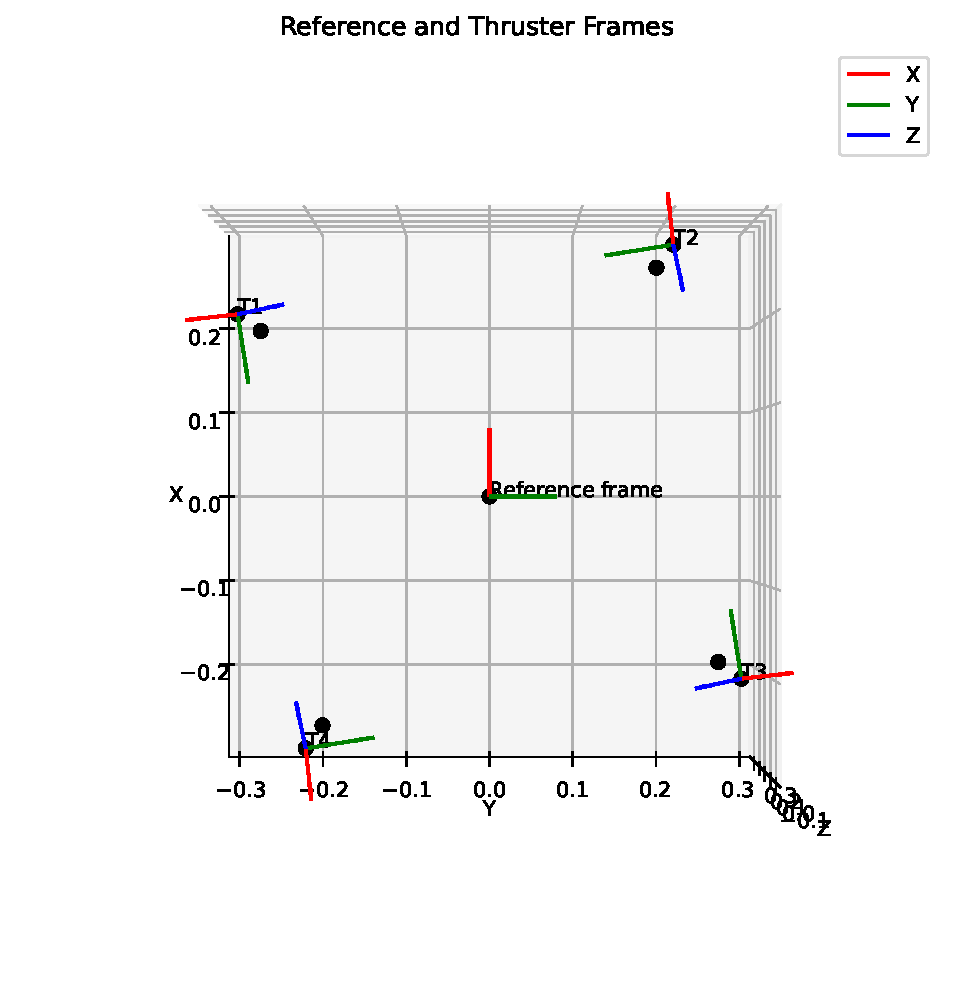
\includegraphics[width=0.35\textwidth, trim={2.5cm 1cm 0cm 0.9cm}, clip]{img/thruster_frames_3.pdf}
        \caption{Thrusters frames obtained after applying the transformations from the reference frame. The blue $Z$-axis also matches the thrust direction.}
            \label{fig:Thrusters_orientations}
\end{figure}

% To ensure the correct configuration, each thruster was labeled with its corresponding VESC motor controllers ID, as specified in the electronics box c.f. Table \ref{tab:thruster_pose_nominal_vesc}.  
For this configuration, the reference frames of the thrusters are illustrated in Figure \ref{fig:Thrusters_orientations}, with IDs according to Table \ref{tab:thruster_pose_nominal_vesc}, where the thrust direction aligns with the local $Z$-axis.


\begin{figure}[htpb]
    \centering
    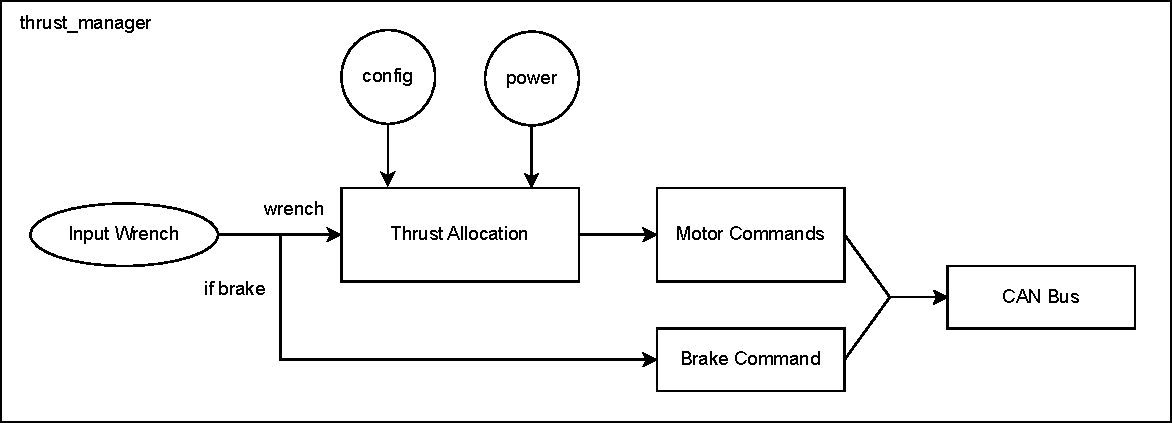
\includegraphics[width=0.9\linewidth]{img/thrust_manager_graph.pdf}
    \caption{Block diagram of \textit{thrust\_manager}}
    \label{fig:thrust_manager_graph}
\end{figure}
\subsubsection{Thruster Allocation Under Power Constraints}
\label{sec:thruster_allocation_power}

This section builds on the approach outlined in Deliverable 3.2. 
Here, we focus on the thrust allocation problem for a given reference wrench. This is a module of the control software referred to as the \textit{thrust\_manager}, see an overview in Figure~\ref{fig:thrust_manager_graph}.

\paragraph{Quadratic Program for Thrust Allocation}

Given a desired reference wrench $\vec{\tau}_{\mathrm{ref}}$, the goal of thrust allocation is to compute the individual thruster inputs $u \in \mathbb{R}^8$ such that the resulting wrench tracks $\vec{\tau}_{\mathrm{ref}}$ as closely as possible while respecting actuator limits. Let $B$ denote the thruster allocation matrix and $W$ a diagonal selection matrix that can deactivate faulty or intentionally disabled thrusters. The nominal allocation problem is formulated as
\begin{subequations}
\label{eq:opt2}
\begin{align}
&\min_{u}\; \frac{1}{2} (BWu - \vec{\tau}_{\mathrm{ref}})^\top H (BWu - \vec{\tau}_{\mathrm{ref}}) 
\label{eq:obj_fun1}\\
\text{subject to} \quad 
& u_{\min} \leq u \leq u_{\max},
\label{eq:ineq_u2}
\end{align}
\end{subequations}
where $H \succ 0$ is a weighting matrix, and $u_{\min}, u_{\max}$ denote the lower and upper thruster bounds, respectively. 
The objective~\eqref{eq:obj_fun1} together with the box constraints~\eqref{eq:ineq_u2} defines a convex \gls{qp}\ian{, e.g., CVXPY}  that can be solved efficiently in real time.\bds{Maybe give some examples of solvers?}



\paragraph{Dynamic Thruster Constraints}
To maintain precise control, ensure that no individual thruster is driven beyond its operational limits, and reduce mechanical wear, the thruster bounds $u_{\min}, u_{\max}$ are adapted dynamically to limit the rate of change of the thruster inputs. 
The bounds are updated based on the previous input $u_{\mathrm{prev}}$ and a maximum allowed rate of change $\triangle u$.

For each thruster $i \in [8]$, \bds{As far as I could see the notation $[n]$ for the set $\{1,2,\dots,n\}$ was not yet defined, unless I overlooked it} \ian{we use $1,2, \cdots,8$} the individual bounds are computed as
\begin{equation}
\begin{aligned}
u_{i,\min} &=
\begin{cases}
    u_{\min} & \text{if } u_{i,\mathrm{prev}} - \triangle u < u_{\min},\\[2pt]
    u_{i,\mathrm{prev}} - \triangle u & \text{otherwise,}
\end{cases} \\
u_{i,\max} &=
\begin{cases}
    u_{\max} & \text{if } u_{i,\mathrm{prev}} + \triangle u > u_{\max},\\[2pt]
    u_{i,\mathrm{prev}} + \triangle u & \text{otherwise.}
\end{cases}
\end{aligned}
\label{eq:maximum_rate_of_change}
\end{equation}
These bounds are defined individually for each thruster and are recomputed at every allocation step. 
In practice, the QP~\eqref{eq:opt2} is solved using the updated bounds $u_{i,\min}$ and $u_{i,\max}$ instead of the static limits $u_{\min}$ and $u_{\max}$.


\paragraph{Available Power and Thruster Power Model}

The smart grapple provides only limited electrical power to the thrusters: the maximum available power is \(P_{\max} = \SI{5}{kW}\), which must be shared between the eight Bluerobotics T500 thrusters and the SensoJoint drives. By contrast, if all eight thrusters operated at their maximum power at \(\SI{24}{V}\), the ROV would require \(8 \times \SI{1044}{W} = \SI{8.35}{kW}\), exceeding the available budget. Hence, the total thruster power must satisfy \(\sum_{i=1}^8 p_i \leq P_{\max}\), where \(p_i\) denotes the power of thruster \(i\).

The mapping between thruster force (or command) and power is nonlinear. For the T500 thrusters, the total power can be approximated as
\[
\sum_{i=1}^8 k_i |u_i|^{3/2} \leq P_{\max},
\]
where \(u_i\) is the control input of thruster \(i\) and \(k_i\) is a fitted constant that depends on whether the thruster operates in forward or reverse mode. Including the power constraint above turns the allocation problem into a nonlinear optimization problem. 
\bds{Insert short sentence to avoid floating equations}
\begin{equation}
\label{eq:NLP}
\tag{\textsc{NLP}}
\begin{aligned}
\min_{u}\;\; &\frac{1}{2} (BWu - \vec{\tau}_{\mathrm{ref}})^\top H (BWu - \vec{\tau}_{\mathrm{ref}}) \\
\text{s.t.}\quad & \sum_{i=1}^8 k_i |u_i|^{3/2} \leq P_{\max}, \\
& u_{\min} \leq u \leq u_{\max}.
\end{aligned}
\end{equation}

To retain the efficiency of a \gls{qp} formulation, we handle the power constraint via a post-processing step, as described below.
\paragraph{Percentage Phase Back (-pp)}
\label{sec:percentage_phase_back}

Since the power constraint in~\eqref{eq:NLP} is nonlinear and incompatible with the \gls{qp} structure, we enforce it in post-processing using a \emph{percentage phase back} strategy~\cite{jenssen2006power}. Let \(u^\star\) be the \gls{qp} solution with total power \(P_{u^\star} = \sum_{i=1}^8 p_i\), and let \(P_{\gls{usg}} \leq P_{\max}\) be the power budget for the thrusters at the time when the optimization is run. If \(P_{u^\star} > P_{\gls{usg}}\), all thruster powers are scaled by
\[
\alpha = \frac{P_{\gls{usg}}}{P_{u^\star}},
\qquad
p_i \leftarrow \alpha\, p_i.
\]
The scaled power of thruster \(i\) is then mapped back to a thrust command \(u_i\) via the fitted T500 power model. For forward and reverse operation this yields
\begin{equation}
u_{i} = \begin{cases}
     \dfrac{-b_{\mathrm{fwd}} + \sqrt{b_{\mathrm{fwd}}^{2} + 4 a_{\mathrm{fwd}} \alpha\, p_{i}}}{2 a_{\mathrm{fwd}}} 
     & \text{(forward)},\\[8pt]
     \dfrac{-b_{\mathrm{rev}} - \sqrt{b_{\mathrm{rev}}^{2} + 4 a_{\mathrm{rev}} \alpha\, p_{i}}}{2 a_{\mathrm{rev}}} 
     & \text{(reverse)},
\end{cases}
\label{eq:percentage_phase_back}
\end{equation}
with \(a_{\mathrm{fwd}}, b_{\mathrm{fwd}}, a_{\mathrm{rev}}, b_{\mathrm{rev}}\) denoting the direction-dependent T500 parameters. This approach allows us to first solve the fast \gls{qp}~\eqref{eq:opt2} without the nonlinear power constraint and then enforce the power limit by a simple scaling and back-transformation, slightly perturbing optimality but preserving real-time feasibility.

To assess the impact of the power constraint and the choice of allocation method, 
we generate a dataset of \(1000\) reference wrenches \(\vec{\tau}_{\mathrm{ref}}\), 
representing desired forces on the \gls{usg}. For illustration, all moments are set to zero,
as the dominant motion is translational. The samples are obtained from a noisy spiral 
path around a sphere. All tests are executed on an Intel(R) Core(TM) i5-6200U 
CPU @ 2.30\,GHz (4 cores), and the thruster power budget is fixed to 
\(P_{\mathrm{thrust}} = \SI{5000}{W}\). We compare the \gls{qp}-pp approach against the 
NLP-based baseline \eqref{eq:NLP} in terms of tracking error~\eqref{eq:obj_fun1} of the desired reference wrench $\vec{\tau}_{\mathrm{ref}}$, power 
consumption, and runtime.

\begin{table}[h!]
\centering
\begin{tabular}{|l|r|r|}
\hline
Approach 
& Error \eqref{eq:obj_fun1} (mean \(\pm\) std.) [\%]
& Power consumption [\%] \\ \hline
\gls{qp}-pp   
& \(+15.6 \pm 11.4\)
& \(+0.2\) \\ \hline
\end{tabular}
\caption{Relative increase in error and average power consumption of \gls{qp}-pp 
compared to the NLP-pow baseline (not shown).}
\label{tab:comparison_power_err}
\end{table}

\begin{table}[h!]
\centering
\begin{tabular}{|l|r|r|r|}
\hline
Approach & Worst case [s] & Avg. runtime [s] & Std. dev. [s] \\ \hline
\gls{qp}-pp    & \textbf{0.0369} & \textbf{0.0181} & \textbf{0.0036} \\ \hline
\eqref{eq:NLP}    & \textit{3.4753} & \textit{0.9000} & \textit{0.4156} \\ \hline
\end{tabular}
\caption{Runtimes for the QP-pp and NLP approaches.}
\label{tab:comparison_power_runtime}
\end{table}

The results \ian{as shown in \cref{tab:comparison_power_err}} \bds{Best refer explicitly to Tables 1 and 2}show that \gls{qp}-pp incurs only a moderate increase in tracking error
(\(+15.6\%\) on average with \(+0.2\%\) higher power consumption) compared to the 
\ian{NLP}\bds{What does "pow" refer to here?} baseline, but achieves roughly two orders of magnitude faster runtimes 
(both on average and in the worst case). Consequently, \gls{qp}-pp is preferred in 
practice, as it enables significantly higher update rates while remaining close to 
the best attainable performance. 

\paragraph{Practical Implementation}
We adopt a modular approach that allows us to overwrite the reference signal at different stages—position, velocity, wrench, or even the duty-cycle command of individual thrusters. This flexibility proved particularly valuable for analyzing and debugging individual modules during the field tests in Marseille (September 2025). The thrusters—and consequently the smart grapple—can be commanded via a \gls{gui}. A position target can be specified (as shown on the left in Figure \ref{fig:thrusters_software}), which is then passed through a cascaded PID controller to generate a target wrench. This wrench is then provided to the optimizer, i.e., the \textit{thrust\_manager} (see Section \ref{sec:thruster_allocation_power}). Alternatively, a velocity command can be set directly—either through the \gls{gui} or using the Logitech gamepad controller—thereby bypassing the position \gls{pid} output. If no \gls{pid} controller is involved, there exists the possibility of providing the reference (to track) wrench directly in the \gls{gui}.

\begin{figure}
    \centering
    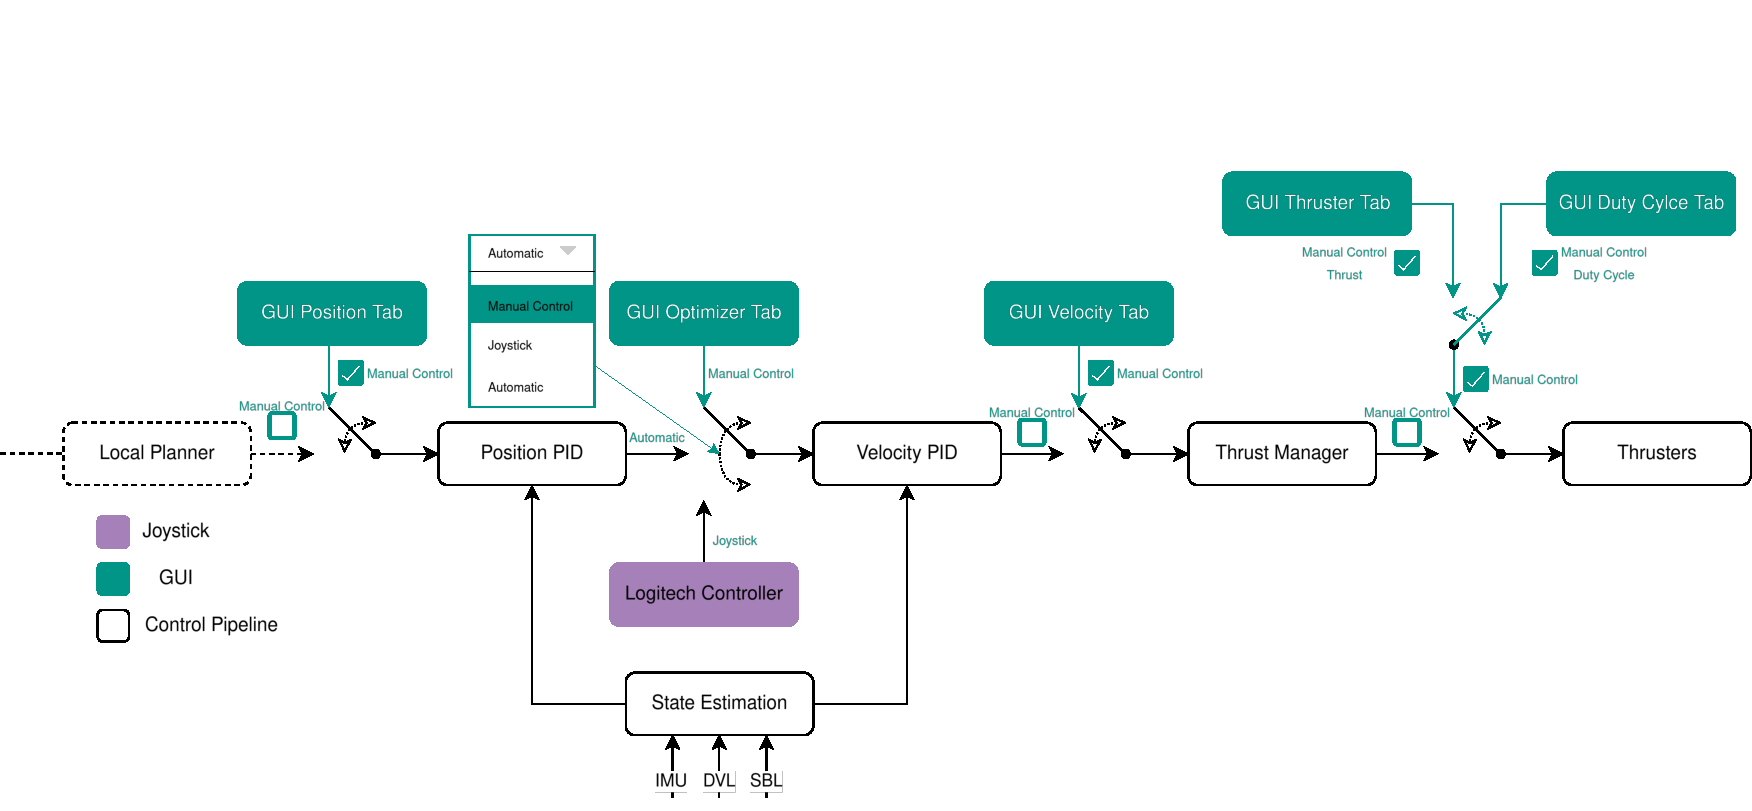
\includegraphics[width=1\linewidth]{img/GUI_documentation.pdf}
    \caption{Architecture of the \gls{usg} control pipeline software.}
    \label{fig:thrusters_software}
\end{figure}

\subsection{Joint control}
The smart grapple joints are actuated by the SensoJoint 5016 BLDC (brushless direct current) motors with a maximal torque of 120 Nm. The motors utilize the \gls{EtherCAT} interface for communication with the computer used for the smart grapple control. In this work, the communication and control of the actuators have been integrated in the overall \gls{ROS2} software architecture using \gls{SOEM} Library \cite{SOEM_library}. All functionalities of the motor can be accessed via a \gls{ROS2} topic or service from any other module of the system. For the convenience of the smart grapple operator, all motor commands can be executed from a \gls{gui} depicted in Figure \ref{fig:sj_gui_screenshot}. 
\subsubsection{Graphic user interface}
The upper button panel contains the ON, OFF, fault reset, and calibration buttons. Pressing ON and OFF will turn the smart grapple on and off, respectively. Turning the smart grapple on means bringing the SensoJoints into the state of enabled operation. From this state, the motors are ready to receive user commands. However, in case of a fault indicated by the built-in fault warning, SensoJoints might enter the fault state, and they will stay in that state unless the fault is cleared by pressing the corresponding button or manually solving the issue onshore. Fault can also be reset automatically by the state machine if it is one of the warnings that can be ignored. The calibration button activates the calibration procedure explained in Section \ref{sec:joint_calibration}.

The lower button panel contains \gls{STO} ON and \gls{STO} OFF buttons. These buttons are connected to the relay inside the electronic box and are responsible for physically connecting and disconnecting the 24V \gls{STO} line. SensoJoint will never be able to reach the operational state without this line connected to the power, as an additional safety measure. \gls{STO} OFF acts as an emergency stop. By default, after the smart grapple has been powered up, the relay is disconnected; therefore, before the operation, the operator is required to press the \gls{STO} ON button.

On the left panel, all the information regarding each joint is displayed, such as the position of the end-effector, velocity, sensed torque, and the fault message. On the central panel, the user has the possibility to control the smart grapple using so-called percentage mode, where \( 0 \%\) corresponds to the fully closed state and \( 100 \%\) to the fully opened state. The joint configuration corresponding to each percentage level is implemented as described in Sec. \ref{sec:percentageControlImplementation}, Case 3. The "Joystick control" checkbox above indicates if the joystick is chosen as the source of input; checking it will disable the slider to avoid conflicting control inputs. The table below the slider displays the joint angles in the smart grapple angle coordinate frame. The smart grapple angle coordinate frame is illustrated in Figure \ref{fig:theta_frame}. \bds{Note that before "Figure" was always put in full, from here in it is being abbreviate; best make this consistent for the entire deliverable} The right panel contains buttons for the relative positioning of the individual joints. By pressing each button, the user opens or closes the joint by 0.05 radians. Using this \gls{gui}, the onshore operator has full monitoring and control over the smart grapple fingers for the manual grasp. 

\begin{figure}
    \centering
    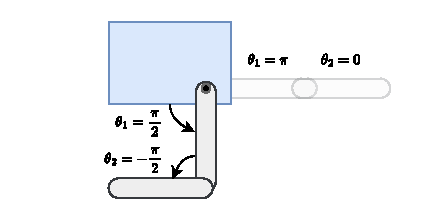
\includegraphics[width=0.6\linewidth]{img/theta_frame_scheme.pdf}
    \caption{Grapple angle coordinate frame.}
    \label{fig:theta_frame}
\end{figure}

\begin{figure}
    \centering
    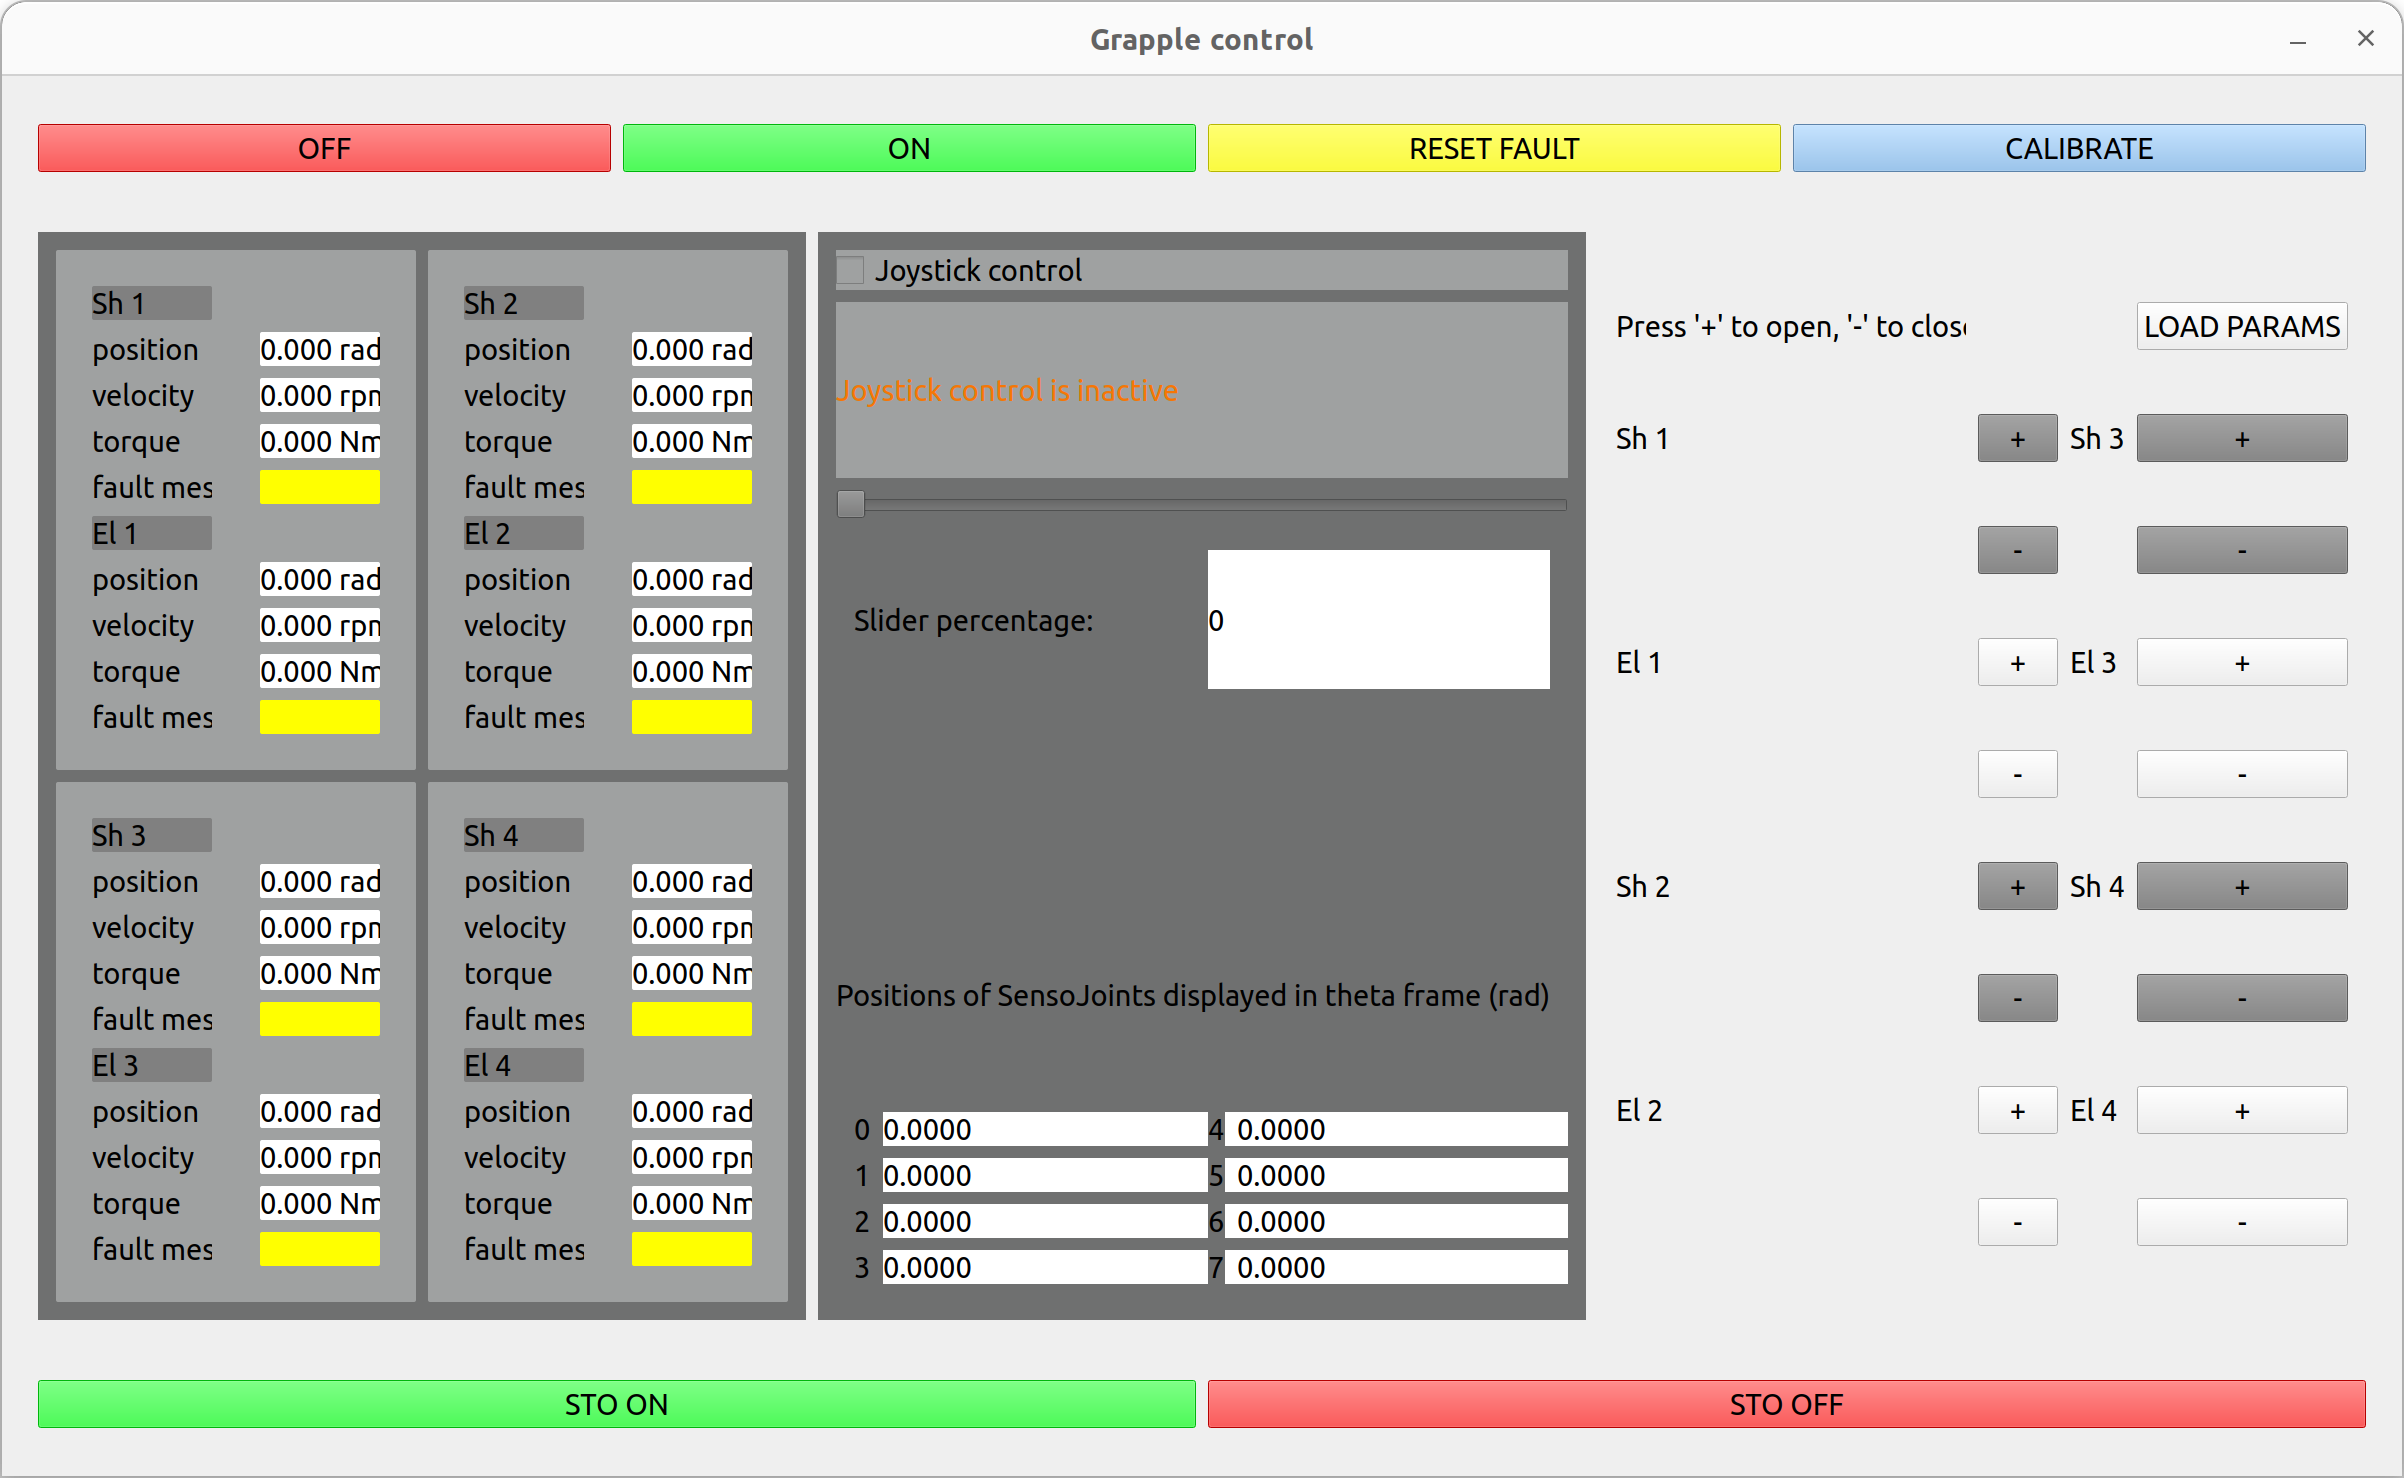
\includegraphics[width=1\linewidth]{img/SJ_GUI_screenshot.png}
    \caption{\gls{gui} for the smart grapple joint control.}
    \label{fig:sj_gui_screenshot}
\end{figure}

\subsubsection{Calibration} \label{sec:joint_calibration}
The calibration routine has been implemented to approximate the angle difference between the encoder zero ("factory zero") and zero in the smart grapple coordinate frame (Figure \ref{fig:theta_frame}). Usually, it must be conducted once, after the smart grapple joint has been reassembled, for example, during routine maintenance. It might also be executed in case of the belt slippage in case of a high joint load. The procedure starts with driving the shoulder joints towards their mechanical limit \bds{remove"above"?} until the predefined torque threshold is reached. Then, the shoulder joints drive back at a small angle to approach the mechanical limit at a lower speed for precision. After that, they are driven on a fixed angle increment between the mechanical limit and the joint angle corresponding to \(\theta_1 = \pi\) in the joint coordinate frame. The same procedure happens then with the elbow joints, but their final position is \(\theta_2 = 0\). After the smart grapple has reached its final starfish-like configuration, the current motor angles are written in the parameter file as \(\Delta\theta_1, \Delta\theta_2\) and later used for angle transformations between encoder angles and smart grapple angles. 

\subsection{State machine of the operation cycle}
The finite state machine is designed to automate the processes of planning, trajectory tracking, precise positioning, grasping, and trash retrieval. The whole cycle of operation is divided into several states, based on the current stage of operation. Transition between states happens in a deterministic manner when particular conditions are fulfilled. The state machine is designed to be responsible for sending activation commands, monitoring the progress, and aborting the operation cycle in case of an error, such as an internal hardware failure. The overall state flow is presented in Figure \ref{fig:general_state_machine}.

\subsubsection{Deploying}
In this state, the initialization procedure happens. The initial storage position of the smart grapple is grasping the collecting net between the SeaCAT \gls{usv} hulls to prevent the unwanted pendulum effect during transportation. Therefore, the deploying state begins with releasing the basket and sending the signal to the SeaCAT \gls{usv} to deploy the grapple under the water. Then, the smart grapple has to be brought into the operational state, which includes a possible joint calibration routine and internal fault check. To be able to transfer to the next state, the smart grapple has to receive the target coordinates as well as the seabed map in the form of an \gls{octomap} \cite{OctomapArticle} from the miniTortuga \gls{uuv}.  
\subsubsection{Planning}
\label{sec:planningState}
As soon as the necessary data are received, no system faults are present, and all components are in the operational state, the smart grapple moves to the planning state. The informed \gls{RRT*} \cite{RRTstarArticle} is currently used in the software to plan a collision-free path, based on the \gls{octomap}, to the first trash object in the received list. Although \gls{RRT*} is used in the current implementation of the control pipeline, it can be replaced by the holistic optimal control approach described in Section \ref{sec:HollisticOptCont}. Once the planning is complete, the state machine activates the tracking state. 

\textbf{Practical implementation} The informed \gls{RRT*} algorithm is implemented using the open-source \gls{ompl} \cite{sucan2012the-open-motion-planning-library}
\subsubsection{Tracking}
\label{sec:trackingState}
The tracking procedure consists of a local planner, state estimation, and the cascaded \gls{pid} controller. The latter then sends the thruster commands according to the architecture illustrated in \ian{Figure} \ref{fig:thrusters_software}. As it is seen from the figure, it is possible to disconnect the direct feedback loop and control the smart grapple using a joystick for debugging purposes. The local planner iterates through the trajectory points provided by the global planner and notifies the state machine as soon as the last one has been reached. Then the tracking state is considered as finished. It is possible that, due to the environmental conditions, such as strong tides, the smart grapple will not position itself directly above the target. In this case, a precise positioning procedure is required to reposition the grapple for the grasp. The next state depends on two factors: whether the user wants to proceed with the manual grasp and whether the visual servoing is feasible. During the development process, the manual grasp is selected, and the smart grapple is navigated solely by the operator onshore using the joystick and the \gls{gui} to control the fingers. The availability of the visual servoing depends on the visibility conditions of the environment. In case of good visibility, the  smart grapple makes a state transition to the visual servoing state, described below. In case of bad visibility, the smart grapple has to position itself based on the last known position of the trash. 

\subsubsection{Visual servoing}
The visual servoing state has the purpose of camera-driven, precise position control of the smart grapple. \bds{it's not clear here when does the visual servoing start and when does the path planning phase stops. Also, how is the reference position expressed for visual servoing compared from the earlier path planning phase. Figure 11 could be linked here?}
\revision{This state is triggered upon reaching the final path point, provided that water clarity is sufficient for object detection. In this phase, the reference position for the controller is expressed in the camera-based coordinate frame. (Figure \ref{fig:general_state_machine}).
Specifically, the object detection model (Section 4.1) identifies the target and provides its bounding box coordinates, while the optimal grasp point estimation algorithm (Section 5.4) determines the desired grasp pose.
The control objective is to center the bounding box within the onboard camera's horizontal frame and reach the desired altitude (pose) vertically using the \gls{dvl} \bds{Use abbreviation LateX package here too} feedback.
Once the desired pose is achieved, the state machine transitions to the grasping state.}

\subsubsection{Grasping}
\textbf{Automated grasp}
The automated grasping state consists of its own state machine illustrated in Figure \ref{fig:alg_torque_monitor}. The general state machine is responsible for initiating the grasping procedure by calling a corresponding \gls{ROS2} service and passing the desired contact points for the grasp from the algorithm described in Section \ref{sec:Gripping_points_opt} (if available). During the automated grasp, it is possible that the actuators activate the built-in maximum torque warning and enter a fault state. In this case, the state machine is responsible for sending the fault-clearing signal unless the fault cannot be cleared automatically (e.g., a finger has to be manually opened to release the torque), and the smart grapple must be switched to manual control. 

\textbf{Manual grasp}
The manual grasp is controlled using the \gls{gui} illustrated in Figure\ref{fig:sj_gui_screenshot}. For the manual grasp to be considered as completed, the user has to initiate the state transition from grasping to dropping by calling a corresponding \gls{ROS2} service.

In case of a successful grasp, the state transitions to the dropping (recovering) state.

\subsubsection{Dropping (Recovering)}
In the dropping state, the state machine sends the signal to the \gls{usv} Tender (illustrated in Figure \ref{fig:SC2concept }), initiating the retrieval of the object grasped. The smart grapple sends the signal to roll the tether, positioning itself above the water, and waits for the \gls{usv} Tender to position itself below. After receiving the signal, approving the object drop, it opens and measures the joint torques. It might happen that due to the seaweed and sediment, the object or parts of it get stuck in the shovels or on the joints. If the excess torque is sensed, the smart grapple will try to repeat the cycle of opening and closing \ian{\(k\)} times \bds{Note that before N was the number of thrusters}, before reporting an error due to the impossibility to continue its operation. The number of tries \(k\) is a system parameter that can be set by a user. After the successful dropping, the smart grapple can proceed with the next object in the list, or the operator can declare the operation finished, and the smart grapple will send a signal to the SeaCAT \gls{usv} to be brought back to shore.

\subsubsection{Error}
The error state is activated in case of an error in any state of operation. The error state means that the state machine notifies the onshore operator about its inability to continue the cycle, and the SeaCAT \gls{usv} brings the smart grapple back to the shore for maintenance. The possible errors include 
\begin{enumerate}
    \item SensoJoint faults that cannot be resolved automatically
    \item Thruster communication failure
    \item Object being stuck in the shovels or in the joints
    \item User-defined error, when the error state is activated by the operator
\end{enumerate}
\begin{figure}
    \centering
    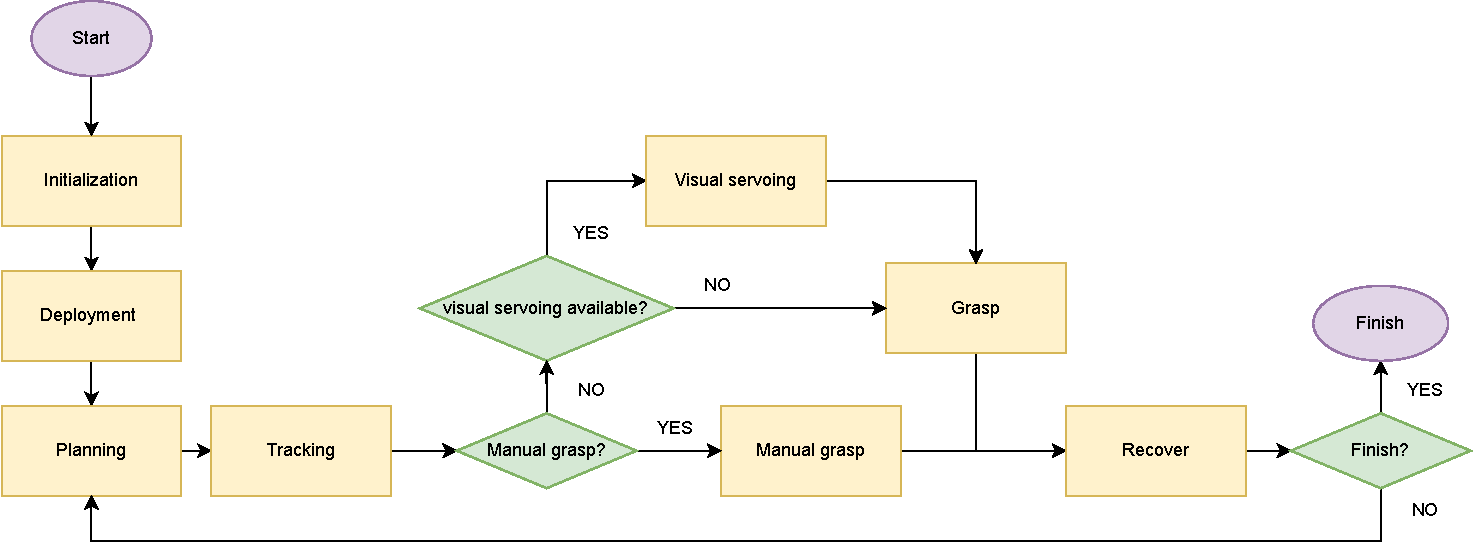
\includegraphics[width=1\linewidth]{img/overall_state_machine.drawio.pdf}
    \caption{Operation state flow.}
    \label{fig:general_state_machine}
\end{figure}


%%%%%%%%%%%%%%%%%%%%%%%%%%%%%%%%%%%%%%%%%%%%%%%%
% Section break
\section{Holistic Optimal Control Approach} \label{sec:HollisticOptCont}

This section presents a unified optimal control framework for the integrated \gls{usv}-\gls{usg} system that accounts for the coupled pendulum dynamics between the surface vessel and the underwater grapple. The approach formulates the trajectory planning problem as a stochastic optimal control problem using \gls{rasaa}, which explicitly handles uncertainties in payload mass, environmental disturbances, obstacle positions, and model parameters. The formulation minimizes energy consumption while satisfying \ian{\gls{cvar}-based} \bds{Make sure to formally define the abbreviation CVaR.} obstacle avoidance constraints, terminal positioning requirements, power limits, and tether tension constraints. A feedback augmentation scheme is introduced to center sampled trajectories around a nominal solution, enabling robust high-frequency online control while the optimization plan operates at lower frequency. \ian{This scheme can be used to replace the traditional trajectory planning method, e.g., RRT*.} \bds{earlier the path planning using RRT* has been introduced and here a difference guidance law, using trajectories is introduced. Which of the two systems are actually controlled via trajectories and, how does the guidance law using RRT* combine with the trajectory planner for the USG?}


\subsection{Modeling of the Integrated \gls{usv}-\gls{usg}}
\label{sec:Modeling}
The goal in modeling is to simulate the \gls{usv}-\gls{usg} behavior with a minimum number of states and as little computational time as possible, without losing any important characteristics. We make the following assumptions for simplification:

\begin{itemize}
	\item the tether is light and thin, such that its gravity, inertia and friction can be neglected
	\item the tether is attached to the \gls{usg} at its center of mass and the orientation of the \gls{usg} is totally defined by the tether. Meaning the \gls{usg}s z-axis $z_{bUSG}$ is pointing parallel to the tether. 
	\item The \gls{usg} rotation around its z-axis is small and does not affect the movement in any relevant manner
\end{itemize}

\subsubsection{Coordinate Frame and State Definition}
We define the following reference frames:
\begin{itemize}
	\item $\{e\}$ is the earth fixed frame \\
	(used if not specified otherwise)
	\item $\{bUSV\}$ is the body frame of USV.
	\item $\{{bUSG}\}$ is the body frame of \gls{usg}
\end{itemize}
Earth and \gls{usv} frame are defined with the z-axis pointing downwards and use of roll-pitch-yaw angles for orientation, as is typical for airplanes. We also define a joint space based on a floating base for the \gls{usv} combined with the \gls{usg} relative position in  spherical coordinates. For the definition of the angles see Figures \ref{fig:AngleDefPhi} and \ref{fig:AngleDefTheta}.

\bds{Best avoid floating/stand-alone equations}
\ian{The state of the \gls{usv}-\gls{usg} system can be written as follows: }
\begin{equation}
	\label{eqJointDefinition}
	\vec q = [x_{USV}, y_{USV}, z_{USV}, \gamma_{USV}, l, \phi, \theta] 
\end{equation}

\begin{tabular}{ll}
	$x, y, z_{USV}$	& position of \gls{usv} w.r.t. earth frame\\
	$\gamma_{USV}$	& yaw angle of USV w.r.t. earth frame\\
	$l$				& tether length \\
	$\phi$			& tilt: angle around fixed USV y axis \\
	 				&(swinging in x-z plane)\\
	$\theta$		& pan: angle around fixed USV x axis \\
					& (swinging in y-z plane)\\
\end{tabular}

The z-position of the \gls{usv} is not actuated but included in the joint vector since the waves are acting on this coordinate and represent a relevant source of disturbance. 


\begin{figure}[ht]
	\centering
	\begin{minipage}{0.3\linewidth}  % Adjust width to fit your images
		\centering
		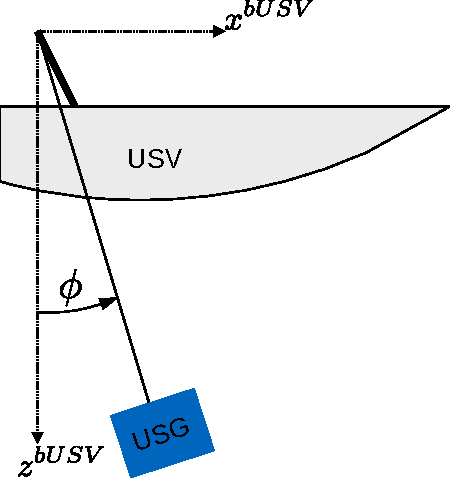
\includegraphics[width=\textwidth]{img/AnglePhiDefinition.pdf}
		\caption{spherical angle definition in x-z plane}
		\label{fig:AngleDefPhi}
	\end{minipage} \hspace{2cm}
	\begin{minipage}{0.3\linewidth}
		\centering
		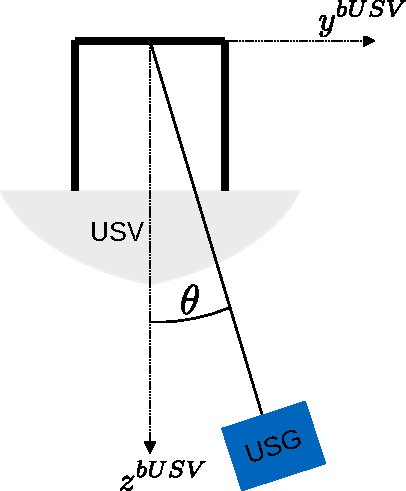
\includegraphics[width=\textwidth]{img/AngleThetaDefinition.pdf}
		\caption{spherical angle definition in y-z plane}
		\label{fig:AngleDefTheta}
	\end{minipage}
\end{figure}


\subsubsection{Modeling Dynamics}

The modeling is performed using the Euler-Lagrange equations, and therefore, the kinetic and potential energies for each part are required. Starting with the \gls{usv}, the kinetic energy is given by its linear and angular motion:
\begin{align}
	K_{USV} &= \frac 1 2 \dot{\vec{x}}_{USV}^T {\Mat{R}_{USV}^{e}} \Mat{M}_{USV} {\Mat{R}_{USV}^{e}}^T \dot{\vec{x}}_{USV} \notag\\
	&+ \frac 1 2 {\vec{\omega}_{USV}^{e}}^T {\Mat{R}_{USV}^{e}} \Mat{I}_{USV} {\Mat{R}_{USV}^{e}}^T \vec{\omega}_{USV}^{e}
\end{align}
where the rotation boils down to only the rotation around the z-axis. The potential energy $P_{USV}$ is given by gravity and buoyancy:
\begin{equation}
	P_{USV} = - m_{USV} g z_{USV} + b_{USV} (z_{USV} - z_{water})^2
\end{equation}
We model the buoyancy similarly to a spring, with the spring constant representing the buoyancy factor
\begin{equation}
	b_{USV} = A_{USV, dis} \rho_{water} g
\end{equation}
\begin{tabular}{ll}
	$m_{USV}$		& weight of the \gls{usv}\\
	$z_{water}$		& height of the water\\
	$A_{USV, dis}$	& displacement area of USV at the water surface\\
	$\rho_{water}$	& density of the water \\
\end{tabular}

The next system component is the tether, including the winch to move it. We model its kinetic energy by a simple inertia $I_l$ acting on the first derivative of the tether length $\dot l$:
\begin{equation}
	K_l = \frac 1 2 I_l \dot l^2
\end{equation}
Last but not least we have the energies of the suspended \gls{usg}. The potential energy is given by the \gls{usg}s mass in water $\overline m_{USG}$
\begin{equation}
	P_{USG} = - \overline m_{USG} \,g \, z_{USG}
\end{equation}
and the kinetic energy is given by its motion:
\begin{align}
	K_{USG} &= \frac 1 2  \dot{\vec{x}}{_{USG}^e }^T {\Mat{R}_{USG}^{e}} \Mat{M}_{USG}^{USG} {\Mat{R}_{USG}^{e}}^T \dot{\vec{x}}_{USG}^e \notag\\
	&+ \frac 1 2 {\omega_{USG}^{e}}^T \Mat{R}_{USG}^{e} \Mat{I}_{USG}^{USG} {\Mat{R}_{USG}^{e}}^T \omega_{USG}^{e}
\end{align}

Since we later work with the joint state, we have to transform it by using the Jacobian:
\begin{align}
	\dot{\vec{x}}_{USG}^{USG} &= \Mat{J}_{USG}^{USG} \dot{\vec{q}}
	\\
	K_{USG} &= \frac 1 2  (\Mat{J}_{USG, lin}^{e} \dot{\vec{q}})^T {\Mat{R}_{USG}^{e}} \Mat{M}_{USG}^{USG} {\Mat{R}_{USG}^{e}}^T \Mat{J}_{USG, lin}^{e} \dot{\vec{q}} \notag\\
	&+ \frac 1 2 {(\Mat{J}_{USG, ang}^{e} \dot{\vec{q}})}^T \Mat{R}_{USG}^{e} \Mat{I}_{USG}^{USG} {\Mat{R}_{USG}^{e}}^T \Mat{J}_{USG, ang}^{e} \dot{\vec{q}}
\end{align}
Similar transformations can be done for all kinetic and potential energies, and we can define the Lagrangian in joint space by:
\begin{align}
	L(\vec q, \dot{\vec{q}}) &= K_{USV}(\vec q, \dot{\vec{q}}) + K_{l}(\dot l) + K_{USG}(\vec q, \dot{\vec{q}}) \notag\\
	& - (P_{USV}(\vec{q}) + P_{USG}(\vec{q}))
	\\
	L(\vec q, \dot{\vec{q}}) &= K(\vec q, \dot{\vec{q}}) - P(\vec{q})
\end{align}
By applying the Euler-Lagrange equation 
\begin{equation}
	\frac{d}{dt} \left( \frac{\partial L}{\partial \dot{\vec{q}}} \right) - \frac{\partial L}{\partial \vec{q}} = \vec{f}
\end{equation}
and reordering the terms, we get the dynamics in standard robotics form:
\begin{equation}
	\Mat{M}(\vec{q}) \ddot{\vec{q}} + \Mat{C}(\vec{q}, \dot{\vec{q}}) + \Mat{G}(\vec{q}) = \vec{f}
\end{equation}

\subsubsection{External Forces}
In addition to the internal forces captured by the Euler-Lagrange equation, some external forces act on the system. These are caused by friction (or drag) and actuation \ian{under the low velocities condition of \gls{usv}.} \bds{what about the quadratic damping, or do we assume here low velocities (<1m/s)for the USV?} 
% Friction Forces
The friction forces are divided into three origins, from \gls{usv}, winch and \gls{usg}:
\begin{equation}
\vec{\eta}_D = \vec{\eta}_{USV} + \vec{\eta}_{l} + \vec{\eta}_{USG}
\end{equation}
For \gls{usv} and winch, a linear friction is assumed. For the winch, it is modeled as
\begin{equation}
\eta_{l}(\dot{l}) = c_l \dot{l}
\end{equation}
In case of the \gls{usv} the friction coefficients differ in the \gls{usv}'s $x$, $y$ and $z$ direction. Thus, the velocities in \gls{usv} body frame have to be used, and this requires the use of the body frame Jacobian $J_{USV}^{USV}$ \bds{Jacobian linearisation should be considered around an operating point, that has not been introduced yet.} \ian{Our method didn't assume linearized Jacobian because the operation range may not be small.} to transform from joint-space to body frame velocities and from body frame forces back to joint space forces. % TODO add footnote about transformation by conservation of energy and equal power
\begin{subequations}
	\begin{align}
	\dot{\vec{x}}_{USV}^{USV} &= \Mat{J}_{USV}^{USV} \dot{\vec{q}}
	\\
	\vec{{F}}_{\eta USV}^{USV} &= \text{diag}(\vec{c}_{USV}) \dot{\vec{x}}_{USV}^{USV}
	\\
	\eta_{USV} &= {\Mat{J}_{USV}^{USV}}^T  \vec{{F}}_{\eta USV}^{USV}
	\end{align}
\end{subequations}
%
Since the \gls{usg} is totally submerged by water, we consider a linear friction model as insufficient. Following \cite{origane2025risk} we model the \gls{usg}'s friction with a second-order expression. Again, the transformation to the body frame is necessary:
\begin{subequations}
	\begin{align}
	\dot{\vec{x}}_{USG}^{USG} &= \Mat{J}_{USG}^{USG} \dot{\vec{q}}
	\\
	\vec{{F}}_{\eta USG}^{USG} &= \text{diag}(\vec{c}_{USG}) \text{diag}(\abs{\dot{\vec{x}}_{USG}^{USG}}) \dot{\vec{x}}_{USG}^{USG}
	\\
	\eta_{USG} &= {\Mat{J}_{USG}^{USG}}^T \vec{{F}}_{\eta USG}^{USG}
	\end{align}
\end{subequations}

The other source of external force is the actuation. The \gls{usv} has two stern thrusters pointing forward and two bow thrusters pointing to the sides. With this constellation the \gls{usv} can move in the $x$ and $y$ directions and rotate around $z$-axis. The \gls{usv}'s $z$ direction can not be actuated. The winch is actuated by an electric motor and a gearbox. In terms of energy efficiency, the winch is the most efficient actuator in the system. The USG has a total of eight thrusters aligned such that a full six degrees of freedom actuation is possible.

To keep the model simple, we consolidate the actuations and consider them to be performed in joint space. This means for every joint defined in (\ref{eqJointDefinition}), except the \gls{usv}'s z position, we model an input force. We further assume a first-order delay between the control signal $\vec u$ and the input force $\vec{f}_{\vec{u}}$. With $\Mat{T}$ as the diagonal matrix with the time constants, we model the input force as
\begin{align}
\dot{\vec{f}}_{\vec{u}}(t) &= \Mat{T}^{-1} (-\vec{f}_{\vec{u}}(t) + \vec{u}(t))
\end{align}

\subsubsection{Model Summary}
All previously modeled parts can now be combined to one set of model equations: 
	\begin{subequations}
	\begin{align}
	& \Mat{M}(\vec{q}) \ddot{\vec{q}} + \Mat{C}(\vec{q}, \dot{\vec{q}}) \dot{\vec{q}} + \Mat{G}(\vec{q}) + \vec{\eta}_D = \vec{f}_{\vec{u}}
	\\
	\ddot{\vec{q}} &= \Mat{M}(\vec{q})^{-1} \left( -	\Mat{C}(\vec{q}, \dot{\vec{q}}) \dot{\vec{q}} - \Mat{G}(\vec{q}) - \vec{\eta}_D + \vec{f}_{\vec{u}} \right)
	\\
	\vec{\eta}_D &= \vec{\eta}_{USV} + \vec{\eta}_{l} + \vec{\eta}_{USG}
	\\
	\dot{\vec{f}}_{\vec{u}}(t) &= \Mat{T}^{-1} (-\vec{f}_{\vec{u}}(t) + \vec{u}(t))
	\end{align}
\end{subequations}

We introduce a combined state $ \vec{z}$ and bring the model equation into control-affine form:
\begin{subequations}
	\begin{align}
	\vec{z} &= [\vec{q}^T, \dot{\vec{q}}^T, \vec{f}_{\vec{u}}^T]^T
	\\
	\dot{\vec{z}} &= [\dot{\vec{q}}^T, \ddot{\vec{q}}^T, \dot{\vec{f}}_{\vec{u}}^T]^T
	\\
	\dot{\vec{z}} &= \vec{f}_{sys}(\vec{z}) + \Mat{G}_{sys}(\vec{z}) \vec{u}
	%			 \vec{f}_{sys}(\vec{z}) &= \begin{bmatrix}
	%			 	\dot{\vec{q}} \\ 
	%			 \end{bmatrix}
	\end{align}
\end{subequations}


\subsection{Technical Approach}
\label{sec:method}

%\section{Design of the solution}

%Having explained the problem, and what others have done in similar situations, now explain your approach. Again, give a general overview of your design first, and then go into detail. The important part here is the concept of your work, not the actual implementation! Make sure that the document (particularly a thesis) is self-contained: It should be possible for a reader familiar with the general area to understand your design. Again, be forthright about the limitations of your design. Also, make sure you justify any shortcuts/limitations convincingly.

With the given model, the next step is to think about the control objective. The goal is to generate trajectories to a desired terminal position. The generated trajectory shall account for
\begin{itemize}
	\item obstacles with uncertain position
	\item uncertain parameters (i.e., uncertain payload mass and friction from gripped object)
	\item process noise
\end{itemize}
We assume all uncertainties mentioned above have a known probability distribution.

\subsubsection{Stochastic Optimal Control Problem}	
We base our solution on the Trajectory Optimization with the \gls{rasaa} introduced by \cite{lew2023risk}. In the same manner, we introduce sampled system models $i \in \{1, \dots N\}$ with parameters $\vec{\xi}^i$ drawn from the parameter distribution. The difference from the original is an alternative cost function and different constraints that fit our proposed model. Before we take a closer look at the cost and constraint functions, we formulate the dynamic system equation as a \gls{sde} with uncertain parameters $\vec{\xi}$ and process noise $\Mat{D} d \vec{\omega}_t$:
\begin{equation}
	\label{eqSDE}
	d\vec{z}_{\vec{u}} = \vec{f}_{sys}(\vec z, \vec{\xi}) dt + \Mat{G}_{sys}(\vec{z}) \vec{u} dt + \Mat{D} d \vec{\omega}_t
\end{equation}
Following the Sampling Average Approach, we define multiple samples $\vec{\xi}^i$ of the uncertain parameters and thus get multiple samples of the \gls{sde} and trajectory:
\begin{equation}
	\label{eqSDEsampled}
	d\vec{z}^i_{\vec{u}} = \vec{f}_{sys}(\vec z^i, \vec{\xi}^i) dt + \Mat{G}_{sys}(\vec{z}^i) \vec{u} dt + \Mat{D} d \vec{\omega}_t^i
\end{equation}
\paragraph{Cost Function}
Based on the sampled trajectories, we define our optimization goal, the cost function, as the expected energy used for the trajectory as
\begin{equation}
\inf_{\vec{u} \in \mathcal{U}} \frac 1 N \sum_{i=1}^{N} \left[ \int_0^{t_f} \dot{\vec{q}}^i \Mat{E}_\eta \vec{f}_{\vec{u}}^i \right]
\end{equation}
with $N$ the number of samples, $\Mat{E}_\eta$ a diagonal weighting matrix representing the energy efficiency, $t_f$ the time horizon, and $\mathcal{U}$ the control space.

\paragraph{Constraints}
For the optimization, we have the following constraints to consider:
\begin{itemize}
	\item obstacle avoidance constraint
	\item terminal constraint (e.g., to reach a desired state)
	\item power and input constraint
	\item tether tension and tether length constraint
\end{itemize}
For obstacle avoidance, we adopt the \gls{cvar}-based constraint formulation proposed in \cite{lew2023risk}. This approach is advantageous because it strikes a balance between conservativeness and feasibility while capturing the varying severity of unsafe events—for instance, distinguishing between a gentle seabed contact and a high-speed collision. In this formulation, the \gls{cvar} constraint enforces chance constraints by ensuring that the probability of constraint violation remains below a specified risk level~$\alpha$. 

Given an ellipsoidal obstacle $\mathcal{O}_j$ centered at $\vec{o}_j$ with shape matrix $\Mat{Q}_j$, and a parameter sample $\vec{\xi}^i$ drawn from the parameter distribution, the obstacle can be represented using a signed distance function:
$$
d_{\mathcal{O}_j(\vec{\xi}^i)}(\vec{z})=1 - (\vec{z}- \vec{o}_j(\vec{\xi}^i))^\top \Mat{Q}_j(\vec{z}- \vec{o}_j(\vec{\xi}^i))
$$
Then, for $M$ obstacles, the constraint function $G$ yields
\begin{align}
    G(\vec{z}_{\vec{u}}^i, \vec{\xi}^i) = \max_{j=1,\ldots M} d_{\mathcal{O}_j(\vec{\xi}^i)}(\vec{z}_{\vec{u}}^i)
\end{align}
Then the \gls{cvar} formulation of this constraint \cite{lew2023risk} reads 
\begin{align}
	&\inf_{s \in \mathbb{R}} \;  s + \frac{1}{\alpha N} \sum_{i=1}^{N} \max \left( \sup_{\tau \in [0, t_f]} {G}_j({\vec{z}}^i_u(\tau), \vec{\xi}^i) - s, 0 \right) \leq 0
\end{align}
where $\alpha$ the risk level and $\vec{z}_{\vec{u}}$ as the position of coupled \gls{usg}-\gls{usv} system.

The terminal constraint is responsible for actually reaching the target position at the end of time horizon $t_f$. To faciliate the resolution of the \ian{\gls{OCP}} \bds{"OCP" was not yet defined}, we consider the terminal position $\vec{z}_d$ as reached, if the expected value lies inside a small environment around the desired position shaped by the diagonal matrix $\Mat{R}_T$. \ian{The goal of closing target position is formulated as follows}
\bds{Avoid floating equations; so best add a short sentence here.}
\begin{subequations}
	\begin{align}
	\frac{1}{N} \sum_{i=1}^{N} & {H}({\vec{z}}^i_u(t_f)) \leq \delta_M,
	\\
	{H}({\vec{z}}^i_{\vec{u}}(t_f)) &= (\vec{z}^i_{\vec{u}}(t_f) - \vec{z}_d)^T \, \Mat{R}_T \, (\vec{z}^i_{\vec{u}}(t_f) - \vec{z}_d)
%	\\
%	\Mat{R}_T &= \text{diag}(1/\delta_x, 1/\delta_y, 1/\delta_z, 1/\delta_l, 1/\delta_\phi, 1/\delta_\theta)
	\end{align}
\end{subequations}
The power constraint takes the power limit of the \gls{usg} into consideration. Since the \gls{usg} actuators are only used to actuate the spherical angles $\phi$ and $\theta$ the constraint is formulated as
\begin{equation}
	\dot{\phi}^i f_{\phi}^i + \dot{\theta}^i f_{\theta}^i \le P_{USG, max}
\end{equation}
Due to the control in joint space, the input constraints are only roughly approximated. With the stacked body frame forces $\vec{f}_{all} = [{\vec{f}_{USV}^{USV}}^T, f_l, {\vec{f}_{USG}^{USG}}^T]^T$ and corresponding stacked Jacobian $\widetilde{\Mat{J}}_{all}(\vec{q})$ we define the constraint as
\begin{equation}
	\abs{\widetilde{\Mat{J}}_{all}(\vec{q}^i)^T} \vec{f}_{all, min} \le \vec{f}_{\vec{q}} \le  \abs{\widetilde{\Mat{J}}_{all}(\vec{q}^i)^T} \vec{f}_{all, max}
\end{equation}
with $ \abs{\widetilde{\Mat{J}}_{all}^T} $ as the element-wise absolute value to give an upper bound.
Last but not least the tether constraints enforce the tether to be always under tension and positive in its length:
\begin{align}
	f_l^i &\le 0
	\\
	l & > 0
\end{align}
\paragraph{Optimization Problem}
By combining all constraints with the cost function, we obtain a tractable optimization problem that computes the optimal control trajectory over the horizon $t_f$, accounting for uncertain dynamics, model mismatch, and uncertain obstacles, as
\begin{subequations}
	\label{eqOCPsaa}
	\begin{align}
	\inf_{\vec{u} \in \mathcal{U}}& \frac 1 N \sum_{i=1}^{N} \left[ \int_0^{t_f} \dot{\vec{q}}^i \Mat{E}_\eta \vec{f}_{\vec{u}}^i \right]
	\\
	\text{s.t.} \notag
	\\
	\inf_{s \in \mathbb{R}} \;  s + \frac{1}{\alpha N} \sum_{i=1}^{N} \max_j &\left( \sup_{\tau \in [0, t_f]} {G}_j({\vec{z}}^i_u(\tau), \vec{\xi}^i) - s, 0 \right) \leq 0 
	\\
	- \delta_M &\leq \; \frac{1}{N} \sum_{i=1}^{N} {H}({\vec{z}}^i_u(t_f)) \leq \delta_M,
	\\
	\dot{\phi}^i f_{\phi}^i + \dot{\theta}^i f_{\theta}^i &\le P_{USG, max}
	\\
	\abs{\widetilde{\Mat{J}}_{all}(\vec{q}^i)^T} \vec{f}_{all, min} &\le \vec{f}_{\vec{q}} \le  \abs{\widetilde{\Mat{J}}_{all}(\vec{q}^i)^T} \vec{f}_{all, max}
	\\
	f_l^i &\le 0
	\\
	& {\vec{z}}_u^i \text{ satisfies dynamics from (\ref{eqSDEsampled}) }
	\end{align}
\end{subequations}
However, the above optimal control problem can be difficult or even infeasible to solve, as large parameter uncertainties may cause divergent trajectories $\vec{z}_{\vec{u}}^i$. To mitigate this, we introduce a feedback control term and optimize over closed-loop controllers.

\subsubsection{Feedback Augmentation}
We first introduce a nominal model and its trajectory $\vec{z}_{\vec{u}}^{nom}$ with nominal parameters $\vec{\xi}^{nom}$ and design a feedback loop, following \cite{origane2025risk}. This draws all trajectories towards the nominal trajectory. We design this feedback controller as a PD controller based on the joint position $\vec q$ and velocities $\dot{\vec{q}}$. Formulated in terms of $\vec z$ we get
\begin{equation}
	\vec{f}_{fb}^i(t) = {\left[\Mat{K}_P ~ \Mat{K}_D ~ \Mat{0} \right]} (\vec{z}^{nom}(t) - \vec{z}^i(t))
\end{equation}
By adding the nominal control input $\vec{u}^{nom}$ we have the control law as
\begin{equation}
	\vec{u}_{fb}(\vec{u}(t), \vec{z}^{nom}(t), \vec{z}^i(t)) = \vec{u}(t) + \Mat{K} (\vec{z}^{nom}(t) - \vec{z}^i(t))
\end{equation}
The nominal models \gls{sde} is identical to (\ref{eqSDE}) with the expected value for the parameters $\vec{\xi} = \vec{\xi}^{nom}$. For the sampled system models $i \in \{1, \dots N\}$ the updated \gls{sde} is formulated as
\begin{equation}
    	d\vec{z}^i = \vec{f}_{sys}(\vec z^i, \xi^i) dt + 
	+ \Mat{G}_{sys}(\vec{z}) \vec{u}_{fb}(\vec{u}(t), \vec{z}^{nom}(t), \vec{z}^i(t)) dt + \Mat{D} d \vec{\omega}_t^i
\end{equation}
 In essence, this extension offers two key benefits:
\begin{enumerate}
    \item it enables high-frequency online control via the local feedback while the main optimization plan at a lower frequency.
    \item it helps \textbf{centering} the trajectories of the sampled models along the \textbf{nominal} one, yielding more compact, feasible trajectories by optimizing over a
class of closed-loop controllers.
\end{enumerate}
More details can be found in \cite{origane2025risk}. Figure \ref{fig:ControlArchitecture} shows the control architecture composed of the offline optimization (dashed line) and the online feedback loop (right blue area). The offline part is divided into simulating the nominal model and simulating the $N$ models with different parameter realizations, $\vec{\xi}$. For the sampled models the feedback loop is displayed in the blue area.

\begin{figure*}[htbp]
	\centering
	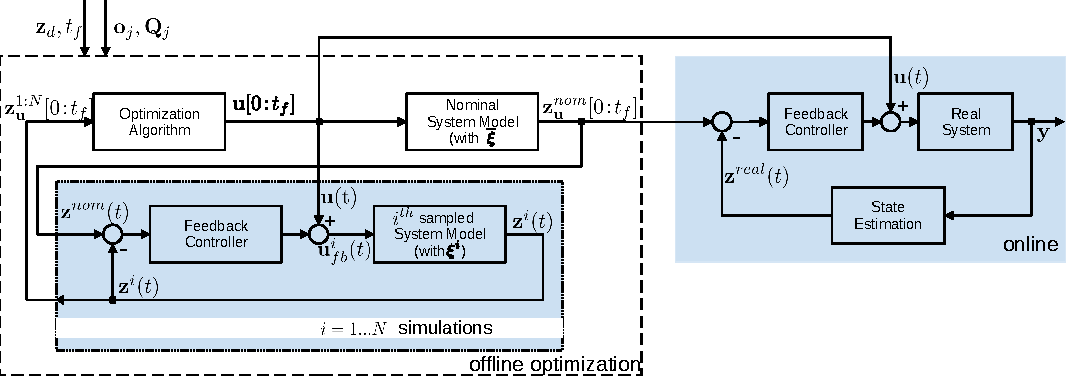
\includegraphics[width=1\linewidth]{img/ControlArchitecture.pdf}  
	\caption{Control Architecture composed of offline planning and online feedback control (adapted from \cite{origane2025risk}). The feedback loop drives the surrogate sampled system to behvae like the nominal one.} 
	\label{fig:ControlArchitecture}
\end{figure*}



\subsubsection{Implementation}
\label{sec:Implementation}




We implement a time-discretized version of the optimal control problem \eqref{eqOCPsaa} with feedback augmentation as depicted in Figure~\ref{fig:ControlArchitecture}. The discretization uses the Euler-Maruyama discretization with time-step $\Delta t$ for the \gls{sde} resulting in
\begin{equation}
    \vec{z}_{k+1}^i = \vec{z}_{k}^i + \vec{f}_{\text{sys}}(\vec{z}_{k}^i, \vec{\xi}^i)\Delta t + \Mat{G}_{\text{sys}}(\vec{z}_{k}) \vec{u}_{\text{fb}}(\vec{u}_k, \vec{z}_k, \vec{z}^i_k) \Delta t + \Mat{D} \vec{\omega}^i_k.
\end{equation}
To balance numerical stability and computational tractability, we use a smaller time step $\Delta t$ for model integration and a larger one for control updates. Specifically, each control input is held constant for $T_{\Delta} \in \mathbb{N}$ integration steps according to a zero-order-hold scheme:
\begin{equation}
\vec{u}_k = \vec{u}_j \quad \text{for } k = jT_{\Delta}, jT_{\Delta} + 1, \ldots, (j+1)T_{\Delta}-1,
\end{equation}
where $j = 0, 1, \ldots, N_{\text{contr}}-1$ is the control interval index. This results in $N_{\text{contr}}$ control input values to be optimized and $S_T = T_{\Delta} N_{\text{contr}}$ total simulation steps.


The implementation is carried out in Python using the JAX library \cite{bradbury2018jax} for numerical computation. JAX enables efficient execution through just-in-time compilation and automatic vectorization, significantly accelerating the computations. To solve the resulting optimization problem, we employ the off-the-shelf solver IPOPT \cite{wachter_implementation_2006}.

\subsubsection{Evaluations: Latest Simulation Results}
\label{sec:Evaluation}
In this section, we aim to validate our model and method through \ian{the simulation.} \bds{what is a Python simulation?} Table \ref{tab:Parameters} in the appendix lists some relevant parameters used for simulation, run on an AMD® Ryzen 9 7950x3d 16-core processor.


\begin{figure}[!htbp]
	\centering
	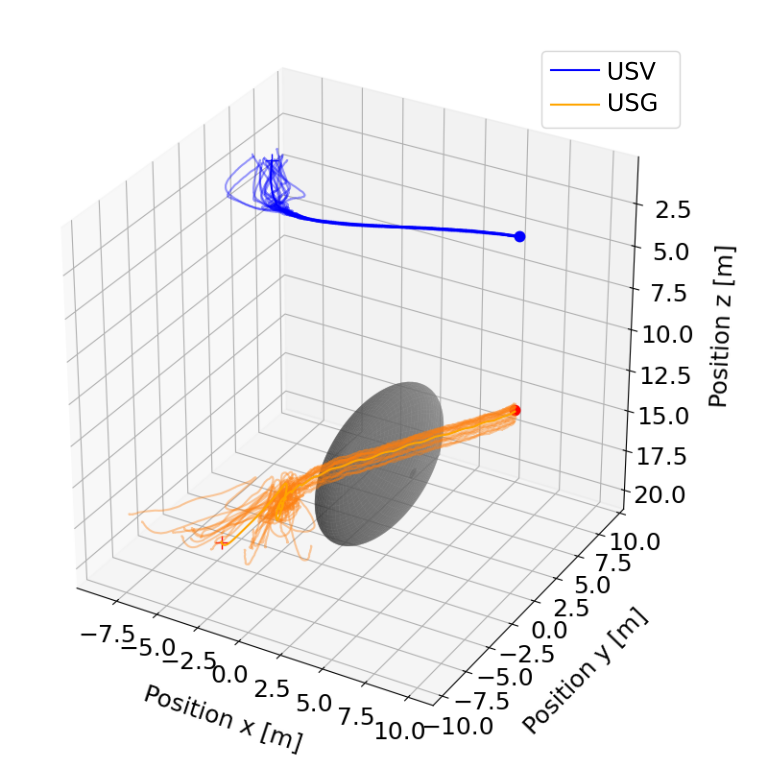
\includegraphics[width=0.35\linewidth, trim={2cm 0.5cm 2cm 1.1cm}]{img/Trajectory3Dusg.png}  % Replace with your file name
	\caption{Planned trajectory from starting point ``+" to terminal point ``$\bullet$"}
	\label{fig:Traje3D}
    \bds{In the figure the blue plus --- and to a lesser extent also the red plus --- is not that clearly visible -> maybe use a different color, like dark blue and dark red?} %\ian{we agree that it may be more visible for changing the color. But it requires rerunning the simulation and some work, we hope the current figure is still understandable.}
\end{figure}

Figure \ref{fig:Traje3D} shows an example for the planned trajectory avoiding the obstacle. Near the starting point marked by ``+'' the uncertain and sampled initial position is shown by the different line origins. Also visible in the graphic are the deviating trajectories the model takes for different realizations of the parameters.

Note that, for the proposed implementation and chosen parameters, the optimization problem involves 742 decision variables and a nonlinear dynamic model with 21 states and $120 \times 50 = 6000$ time steps. This configuration poses a significant challenge for the solver, with computation times ranging from approximately 4 h for a small number of sampled models ($N \approx 5$) to around 17 h for larger values ($N \approx 20$). Nevertheless, the proposed method successfully produces feasible trajectories that reach the desired terminal positions while avoiding obstacles. The simulated system behavior accurately captures the underlying pendulum dynamics and demonstrates the benefits of jointly controlling the \gls{usv} and \gls{uuv}. Future work may focus on improving computational efficiency, possibly through a different solver strategy or an approximation of the model.

%%%%%%%%%%%%%%%%%%%%%%%%%%%%%%%%%%%%%%%%%%%%%%%%%%%%%%%%%%%%%%%%%%


\section{Perception System for Litter Object Localization}
The grapple needs to be able to localize litter objects autonomously underwater, infer the relative position of an object to the grapple, and estimate the litter object metric geometry in preparation for grasping. To this end, we present in the following an overview of the perception system design as shown in Figure~\ref{fig:perception_pipeline}. First, we subscribe to depth and RGB data produced by a passive stereo camera. Secondly, we perform inference with a YOLOv8 object detection deep learning model, trained to detect litter objects underwater. Third, we use the bounding box returned by the object detection inference to create a mask for the depth map produced by the stereo camera, masking the pixel values in the depth mask which don't correspond to the detected object. Fourth, we use the depth map and the masked depth map to construct a voxel map of the scene with static and dynamic elements. Finally, the voxel map, RGB data and object detection model output can be monitored in real-time via Gstreamer and/or Foxglove. The majority of the process, bar the stereo depth estimation computed on-board the stereo camera, is performed on an embedded GPU system, enabling the deployed algorithms to benefit from a high degree of parallelization w.r.t. the computations, ultimately increasing the speed of the pipeline. 

\begin{figure}
    \centering
    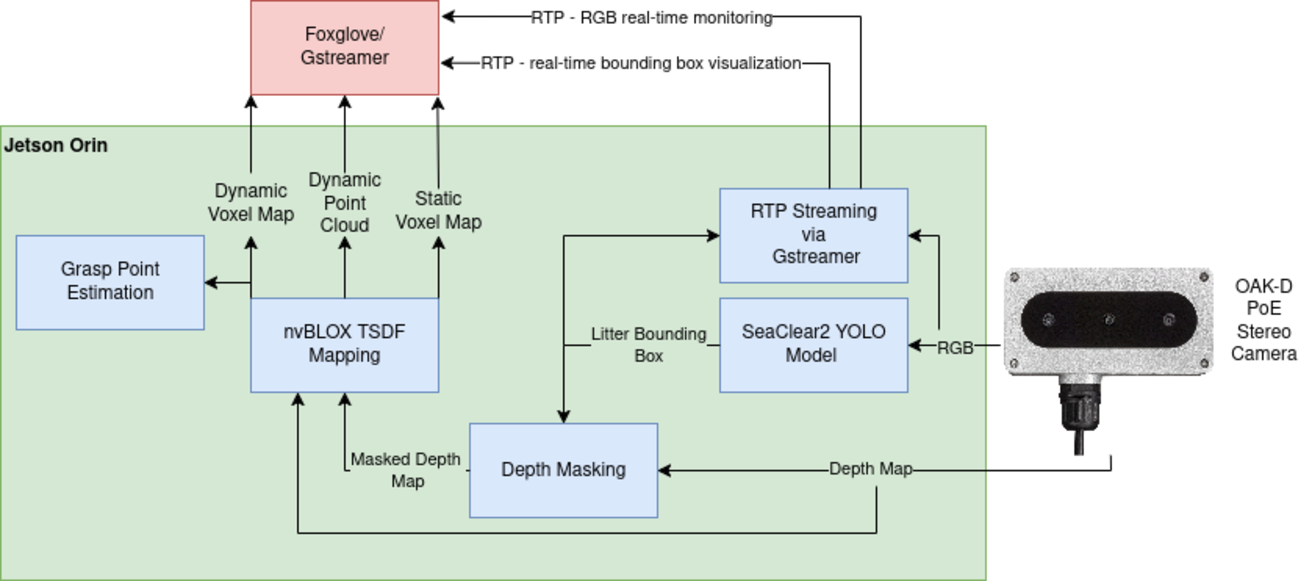
\includegraphics[width=0.9\linewidth]{img/vision_pipeline/vision_system.pdf}
    \caption{An overview of the perception system. The blue boxes represent the processing nodes. The red box the monitoring node(s). The green background indicates the processes that benefit from edge GPU acceleration.}
    \label{fig:perception_pipeline}
\end{figure}

\subsection{Underwater Object Detection}
\label{sec:object_detection}

The SeaClear YOLO based object detection deep learning model for underwater litter objects as described in the Report D4.3, was used as a foundation for the current perception pipeline. The object detection model returns a bounding box around a region in an RGB image at the location of a detected litter object. The bounding box is then 1) laid on top of the actual RGB data and streamed to the surface machine for real-time monitoring, 2) passed to a depth masking node which separates an incoming depth map aligned with the RGB data into "litter object" and "non-litter object" parts. The masked depth mask is then passed to the 3D reconstruction algorithm discussed in Section~\ref{sec:TSDF}.

\subsection{Truncated Signed Distance Function based 3D Reconstruction}
\label{sec:TSDF}

\textbf{Static Voxel Mapping}
\label{sec:static_tsdf}

Compared to point cloud representations, voxel maps approximate each point in 3D space as a voxel, the 3-dimensional equivalent of a pixel. We use the \gls{TSDF}  \bds{For consistency also use the abbreviations latex package in this section} in our approach, which assigns a value corresponding to the (signed) distance of that voxel to the nearest surface. The surface of an object can then be extracted as the location of voxels with distance value 0. This approach provides an estimate for the volumetric properties of objects, informing our grasp planning. 
Additionally occupancy information of the voxels is stored, such as in occupancy grids, where the probability of a voxel being occupied is stored. Each voxel in space is classified as either {\it occupied} or {\it free}, meaning that a particular voxel is either outside of a 3D object if it is {\it free} and situated within the object if it is {\it occupied}.
This dual representation benefits our functionality two-fold. On the one hand the TSDF based voxel map provides a metric estimate of an objects geometry, allowing us to extract volumetric information informing our grasp planning. The occupancy probabilities can be used for obstacle avoidance. \hamish{Described below is the computed 3D reconstruction of objects w.r.t. to the camera frame. In order to relate the spatial and volumetric information of detected objects from the camera frame to the robots frame, we apply a transformation consisting of a rotation and a translation from the camera's base frame to the robot's base frame, defined in the transformation tree of the software stack. This allows the spatial information of objects to be used for planning and visual servoing of the grapple system.}  \bds{how do we convert the objects detected into camera frame into the local map, so that these can be used in the planning or visual servoing phases?} \\
 
Truncated Signed Distance Fields are based on \gls{SDF} which work in the following way. Given a depth map $\mathcal{D}$ , the center point of a voxel w.r.t. the voxel grid coordinate frame $\boldsymbol{p_L}$ and the camera pose w.r.t. the voxel map  $\boldsymbol{T_{CL}}$, we can sample the depth information from the depth map by projecting $\boldsymbol{p_L}$ onto the depth map and assigning the depth value at that point to the corresponding voxel~\cite{Millane2023} 

\begin{equation}
    d = \mathcal{D} \left[ \pi_{camera} \left( \boldsymbol{T}_{CL} \boldsymbol{p_L}  \right) \right]
\end{equation}

where $\mathcal{D} \left[ \boldsymbol{u} \right]$ represents sampling from the depth map at point $\boldsymbol{u}$. The camera projection function $\pi_{camera} \left( \boldsymbol{p_C} \right)$ for a arbitrary point in 3D space $\boldsymbol{p_C}$ is defined as 

\begin{gather}
    \pi_{camera} (\boldsymbol{p}_C) = \frac{1}{ p_{C,z} } 
    \begin{bmatrix}
        f_x& 0& c_x \\
        0& f_y& c_y
    \end{bmatrix}
    \begin{bmatrix}
        p_{C,x} \\ p_{C,y}\\ 1
    \end{bmatrix} 
\end{gather}

where $f_x$, $f_y$, $c_x$ and $c_y$ are the pinhole camera intrinsic parameters which we receive from camera calibration. Now that we have the depth value sampled at the location of the voxel center projected onto the depth map, we subtract the distance of the voxel center to the camera in order to receive the signed distance field value

\begin{equation}
    sdf_i(\boldsymbol{p}_L) = \mathcal{D} \left[ \pi_{camera} \left( \boldsymbol{T}_{CL} \boldsymbol{p_L}  \right) \right] - cam_z( \boldsymbol{p}_L ).
\end{equation}

The result $sdf_i(\boldsymbol{p}_L)$ is the signed distance field value for the voxel. Repeating this procedure for each pixel in-view, i.e. each voxel which can be projected onto the depth map at a given timestep, we can classify each voxel in-view as occupied or unoccupied, extracting the surface of an object as the zero-crossing between occupied and unoccupied values. TSDF is sufficient for surface reconstruction, where all voxel outside of a truncation distance $\epsilon$ are not assigned a value. 

For TSDF, the $sdf_i$ are only considered for voxels within small truncation distance $\epsilon$ away from the surface of objects. The truncated version of the $ sdf_i $ for the $i$-th observation of a scene is defined as $ tsdf_i $ ~\cite{Werner2014}:

\begin{equation}
    tsdf_i(\boldsymbol{p}_L) = \max\left(-1,   \min \left( 1 , \frac{sdf_i(\boldsymbol{p}_L)}{ \epsilon} \right) \right)
\end{equation}

\begin{figure}
    \centering
    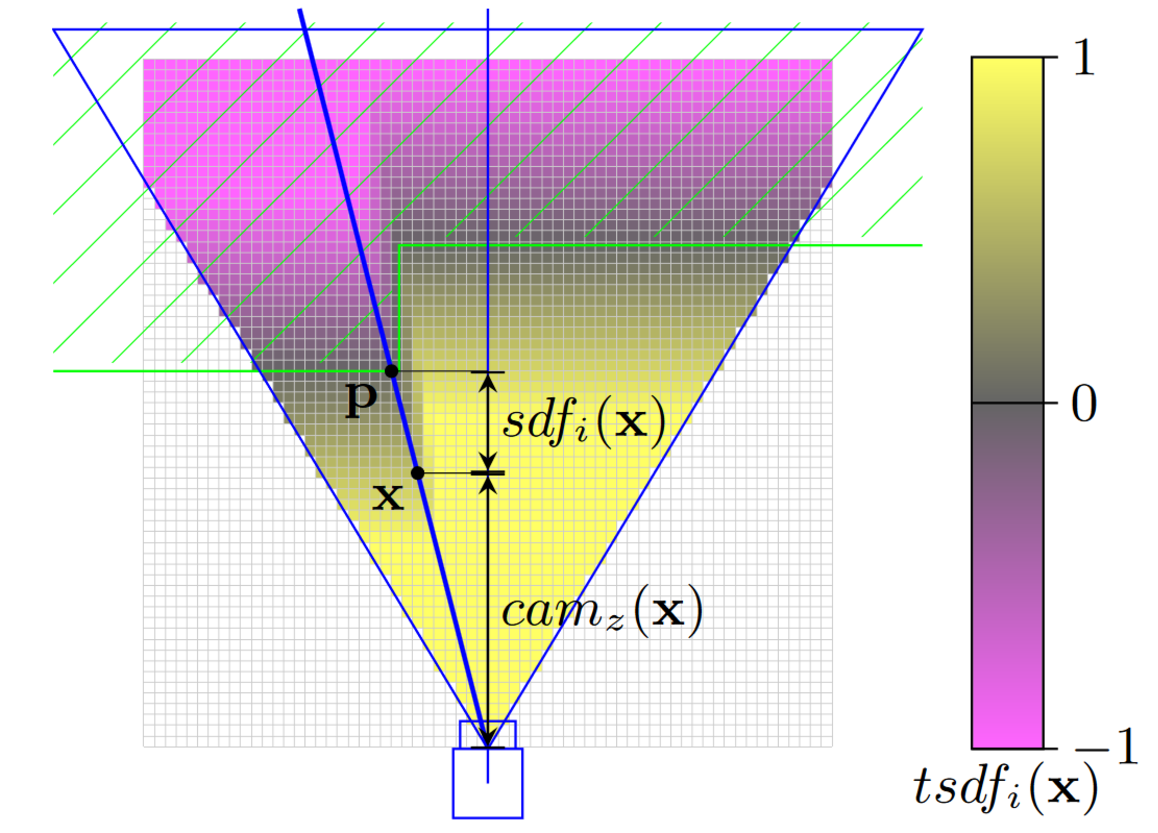
\includegraphics[width=0.5\linewidth]{img/vision_pipeline/tsdf_illustration.pdf}
    \caption{The 3D object in space is denoted in green. The truncated distance values are denoted in color from pink to yellow. In this case an exemplary truncation distance $ \epsilon $ is set to $1$~\cite{Werner2014}.}
    \label{fig:sdf_illustration}
\end{figure}

An illustration of how signed distance fields work can be seen in Figure \ref{fig:sdf_illustration}, here computing the distance of voxel $\boldsymbol{x}$ to the surface point $\boldsymbol{p}$ is illustrated. The colored regions in Figure \ref{fig:sdf_illustration} indicate the values within the truncation threshold.

Voxel grids can be efficiently implemented for GPU acceleration. The grid is divided into larger  chunks of voxels, e.g. an 8x8x8 block, and each chunk is stored within GPU memory; each block is then continuously updated in parallel by the GPU, freeing up voxels that are no longer occupied, assigning depth values to newly observed voxels and updating distances as the camera moves through the scene.

\newpage

\textbf{Dynamic Voxel Mapping}
\label{sec:dynamic_tsdf}

\begin{figure}[!htbp]
    \centering
    \begin{minipage}{0.4\textwidth}
        \centering
        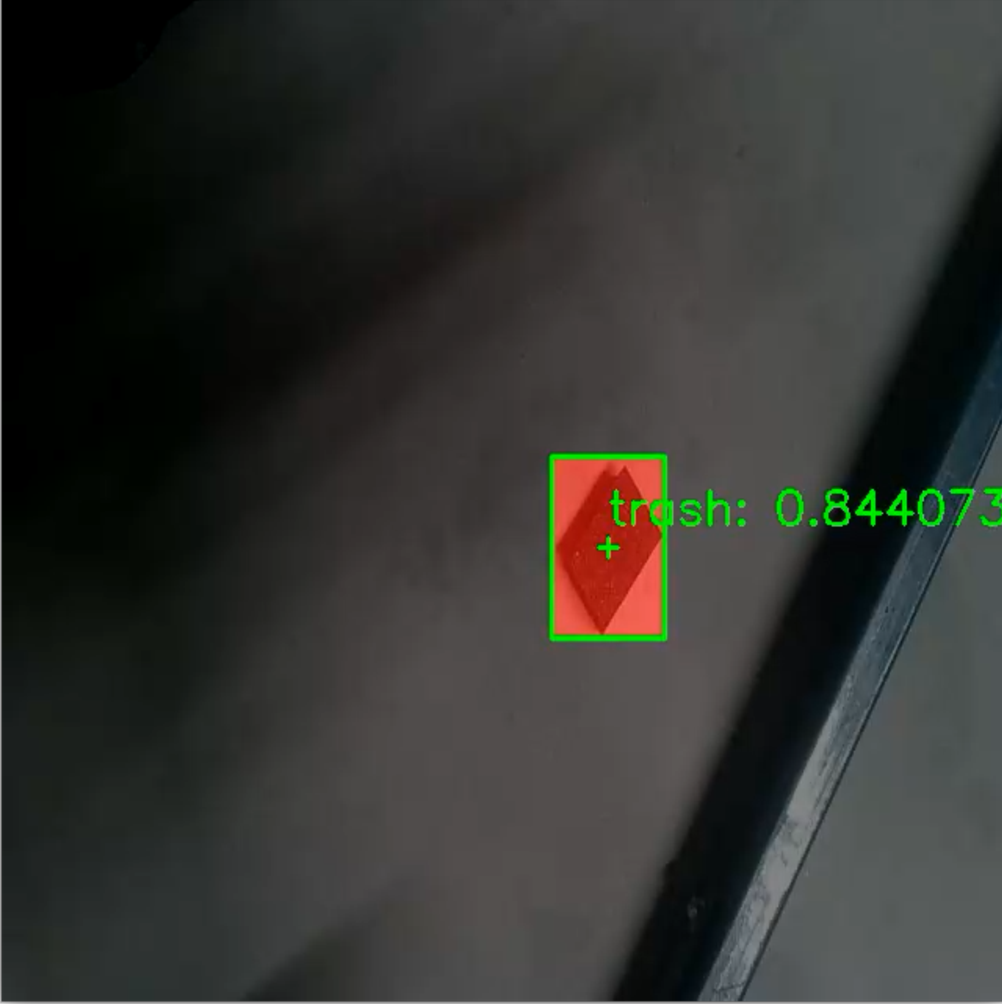
\includegraphics[width=\linewidth]{img/vision_pipeline/detection_in_air.pdf}
        \caption{The bounding box returned by the object detection model post-processed and laid on top of the RGB data from the downward facing stereo camera. }
        \label{fig:object_detection}
    \end{minipage}\hfill% <-- Keep this comment here!
    \begin{minipage}{0.4\textwidth}
        \centering
        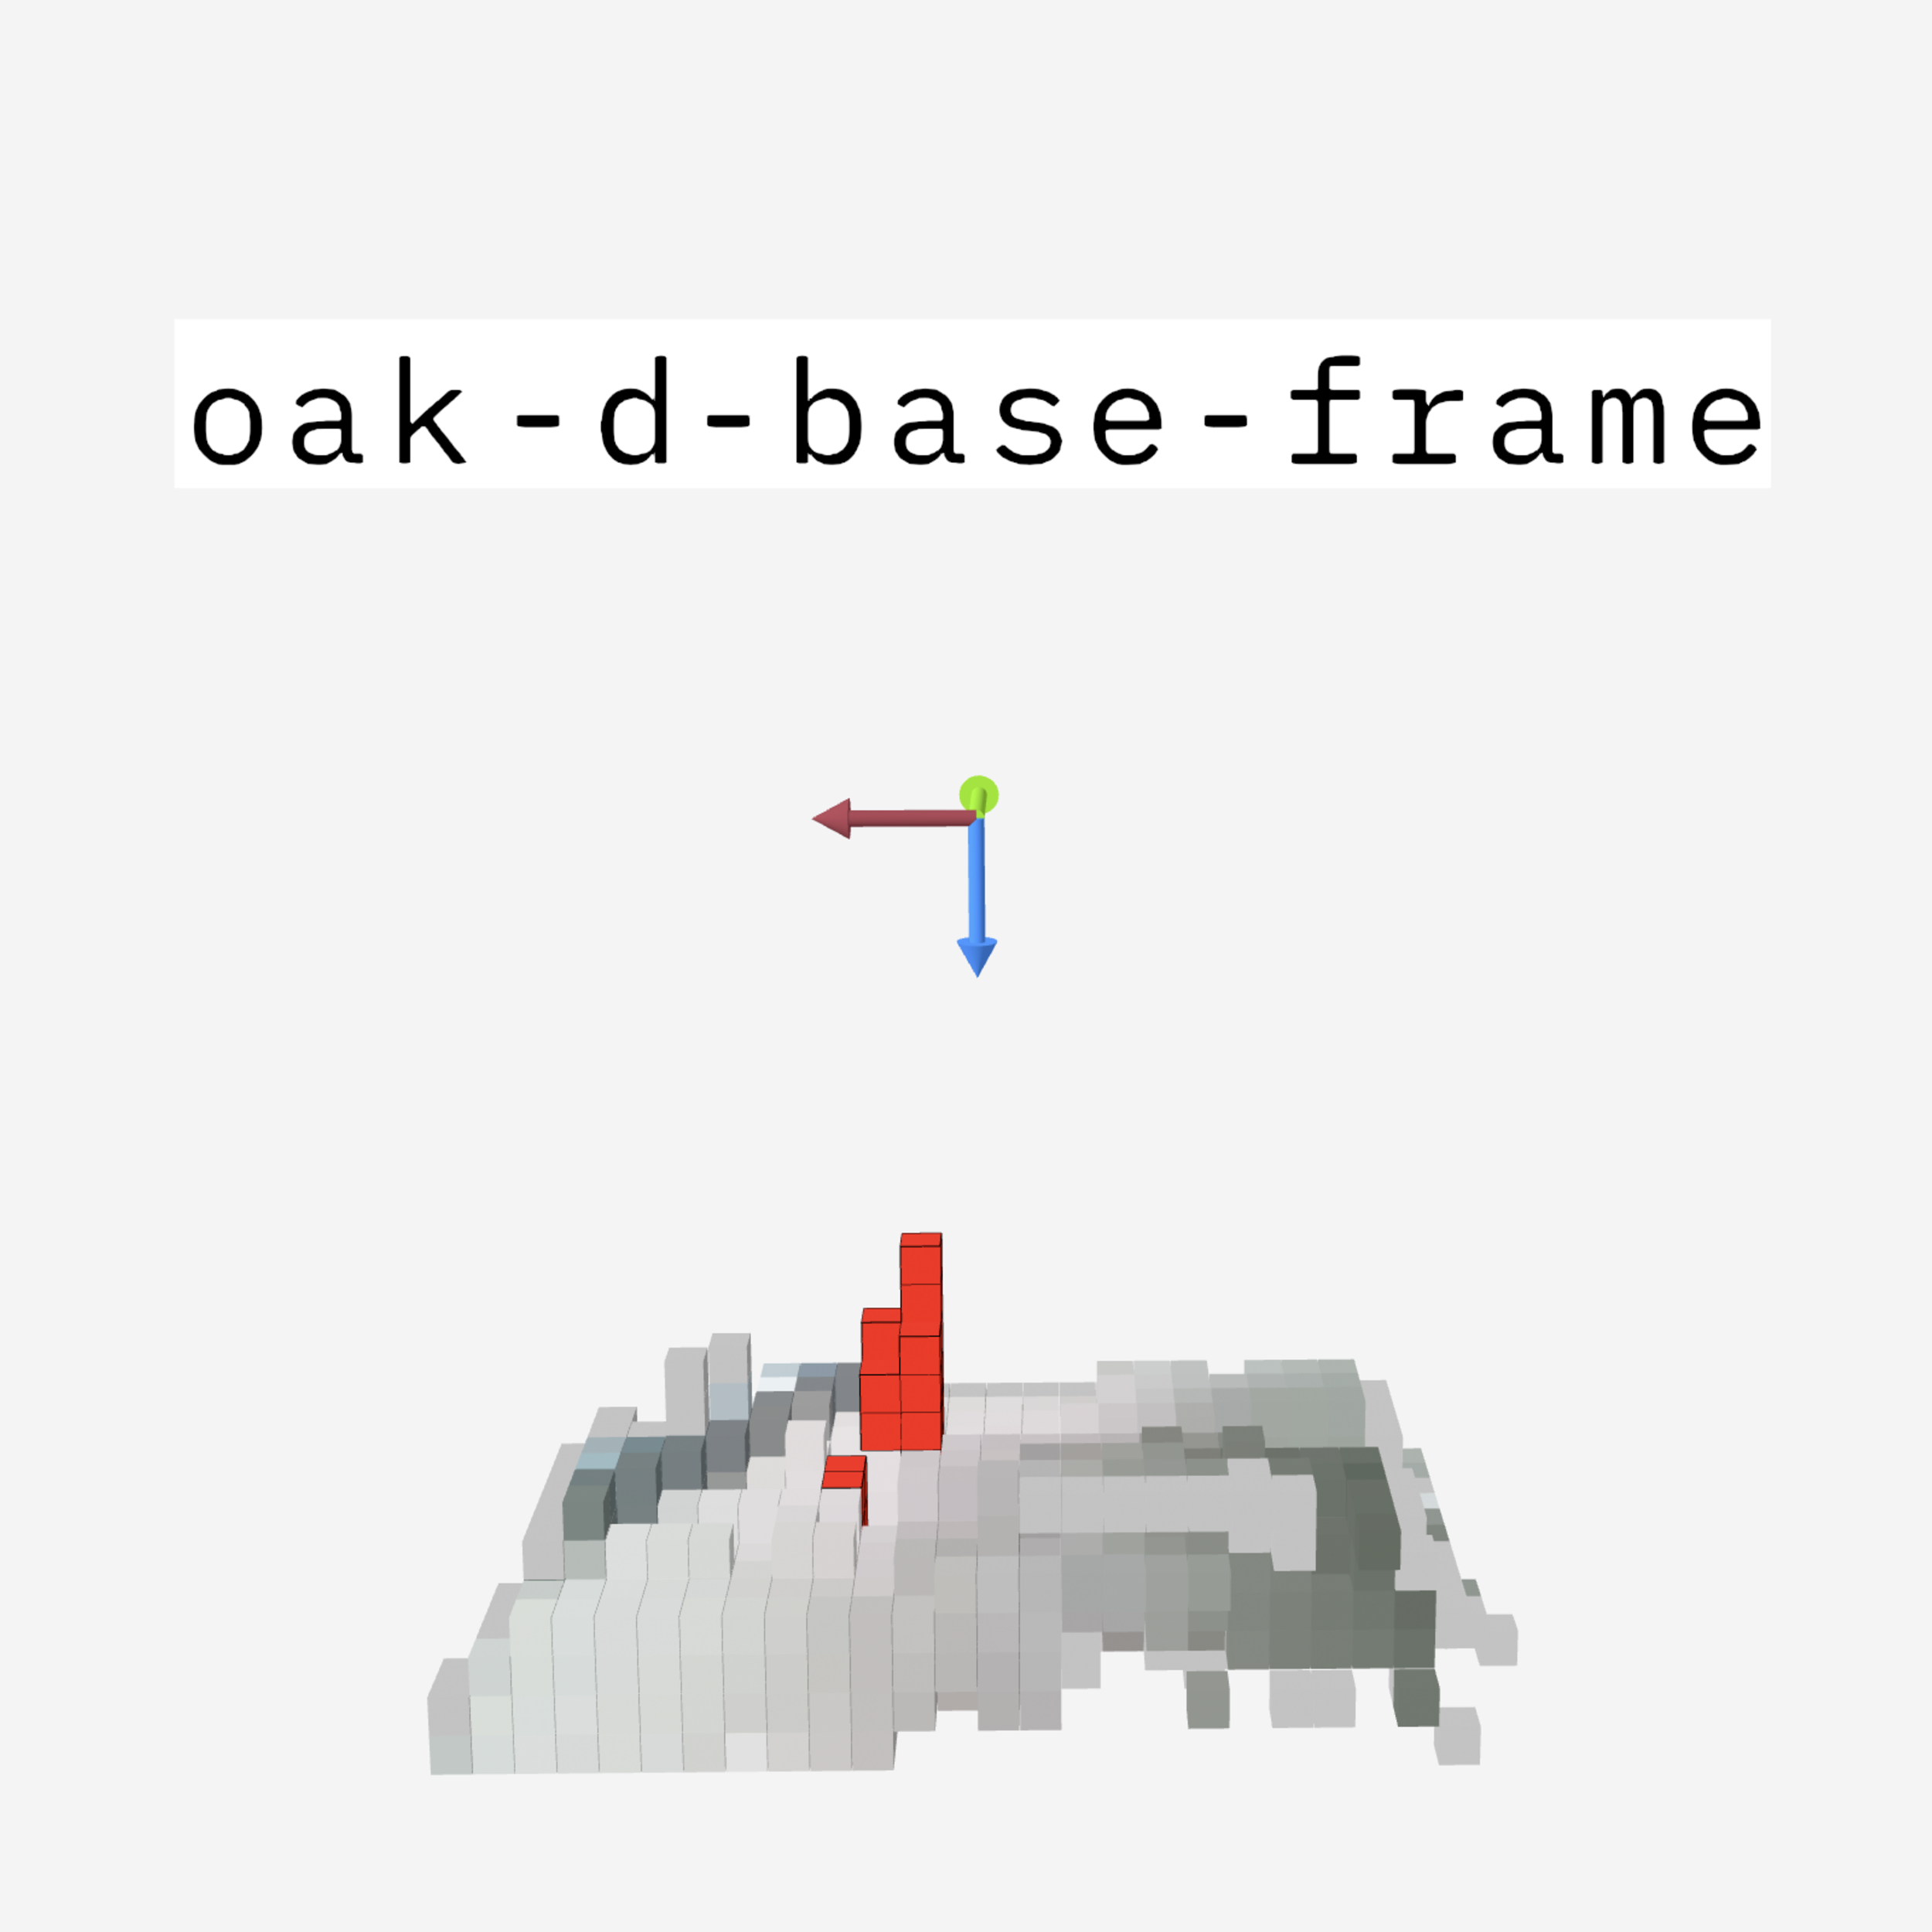
\includegraphics[width=\linewidth]{img/vision_pipeline/tsdf_in_air.pdf}
        \caption{The static and dynamic voxel layers computed from the input scene in Figure \ref{fig:object_detection}. The red voxels correspond to the litter object detected by the model.}
        \label{fig:image2}
    \end{minipage}
    \label{fig:object_detection_tsdf}
\end{figure}

So far we have only discussed mapping of a static scene by the \gls{TSDF} algorithm. Mapping the whole scene is computationally expensive even in the \gls{TSDF} case. Since we receive a bounding from from the object detection model, we use this to reduce the region of interest for applying \gls{TSDF}. The bounding box received from the object detection applied to the RGB data as discussed in Section~\ref{sec:object_detection}, is used to mask the depth map from the stereo camera into litter object parts and non-litter object parts. The voxel map is then separated into a static and a dynamic layer, where the static layer is computed as before, but the dynamic layer now only contains voxels computed from the masked depth values, i.e. contains voxels that correspond to a detected object. We can then apply grasp point estimation to the dynamic layer corresponding to the detected object. 

We relax the assumption that only static objects are reconstructed by the algorithm from Section~\ref{sec:static_tsdf}, since this allows the bounding box to move within the scene if e.g. the object is moved by ocean dynamics. For this, we need to apply a decay step to the occupancy values of the voxels. At a fixed frequency, all voxel occupancy probabilities are decayed towards 0.5 over time. This means that the state of a voxel (occupied or free) becomes less certain after it has fallen out of view until it becomes unknown i.e. the voxel holds 0.5 occupancy probability. 



%%%%%%%%%%%%%%%%%%%%%%%%%%%%%%%%%%%%%%%%%%%%%%%%%%%%%%%%%%%%%%%%%%
\section{Smart Grapple Grasping Approach}

This section details the grasping methodology developed for the Smart Grapple to reliably capture underwater litter of varying sizes and weights. The approach integrates a torque-monitor-based adaptive grasping algorithm that employs a three-state machine architecture (closing, loading, and finalization phases) to ensure stable grasp execution through continuous torque feedback. Building upon the kinematic foundations, the section further presents an optimal grasping posture analysis that determines finger configurations maximizing gripping force under joint position and torque constraints, addressing three operational scenarios with varying levels of perception information. Finally, a gripping points optimization service is described that leverages 3D point cloud data to identify optimal contact surfaces for the four-finger configuration.


\subsection{Torque Monitor Grasping Algorithm}
The torque-monitor-based grasping algorithm, \ian{which is the module in "grasping" block in Figure \ref{fig:general_state_machine}}, is designed to enable adaptive and reliable grasp execution by continuously monitoring the joint torques of the smart grapple during the closing process. The function follows a state-machine architecture that ensures the grasping motion transitions smoothly across distinct control phases, each governed by torque feedback and kinematic state information. This design enhances grasp stability while preventing excessive force that could damage the object or the gripper mechanism.

\bds{In the next paragraph maybe also connect explicitly to the finite state machine introduced before? or else refer to Figure 20 explicitly.\\}
\ian{As shown in Figure \ref{fig:alg_torque_monitor}, the} grasping process begins with the initialization of the system state and movement of the smart grapple to a predefined start configuration. Once positioned, the state machine is activated to coordinate the grasp sequence. The algorithm proceeds through three principal states: State 1 (Closing Phase), State 2 (Loading Phase), and State 3 (Finalization Phase). Each state defines a specific control behavior based on torque feedback and configuration updates.

\begin{enumerate}
    \item State 1 – Closing Phase:\\
    The smart grapple starts from an open position and begins closing toward the object. The current joint configuration is recorded, and a corresponding closing command is generated and stored in the command buffer. This command drives the fingers toward the target until the torque values begin to rise, indicating initial contact with the object. Once the torque measured on any joint exceeds the predefined threshold, the algorithm transitions to State 2. If no contact is detected during the closing process, the smart grapple continues to close until reaching its fully closed configuration, after which the state machine switches to State 3.
    \item State 2 - Loading Phase:\\
    The algorithm continuously monitors the torque signals to determine whether the object has been securely grasped. If the measured torque exceeds the predefined threshold, indicating that the object is firmly held with sufficient contact force, the current configuration is maintained to stably hold the object. The state machine remains in this phase until an open command is received. Conversely, if the detected torque falls below the threshold—suggesting that the contact is insufficient—the system reverts to State 1 to resume the closing process and reattempt the grasp.
    \item State 3 - Finalization Phase:\\
    In the final stage, the fully closed configuration is assigned to the command buffer to ensure completion of the grasp. The algorithm then flags the state machine as finished, marking the termination of the grasp cycle. The final joint configuration is maintained to preserve a stable grasp until further instructions are issued.
\end{enumerate}
In each state, the joint command is computed based on torque feedback and kinematic information, and then stored in the command buffer. The command buffer is transmitted to the motor driver at each sampling iteration, ensuring real-time execution of the grasping control loop.
\begin{figure}[!htbp]
    \centering
    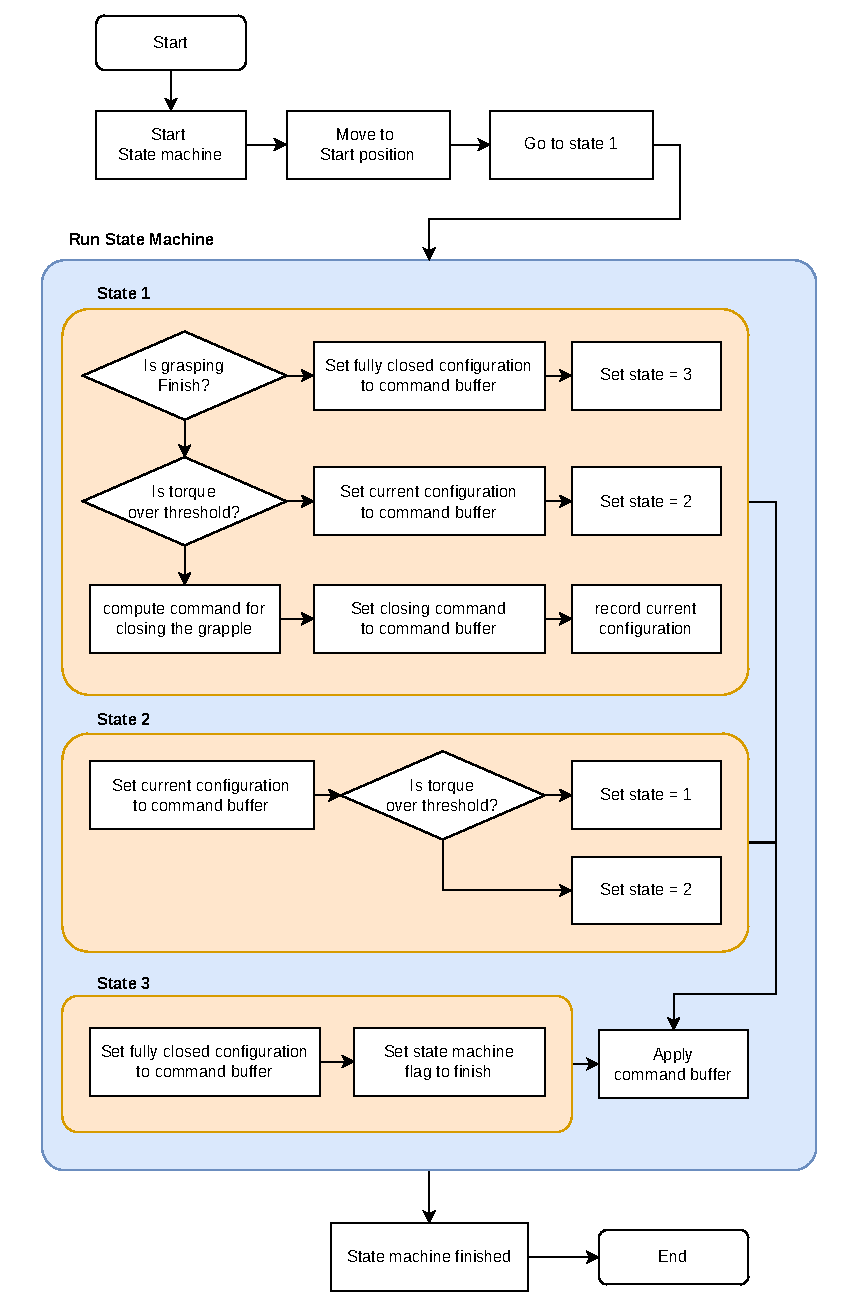
\includegraphics[width=0.87\linewidth]{img/torque_monitor_alg.pdf}  % Replace with your file name
	\caption{The pipeline of the torque monitor grasping algorithm. }
	\label{fig:alg_torque_monitor}
\end{figure}


\subsection{Grapple Kinematics}

This subsection presents the kinematic modeling of the Smart Grapple finger mechanism, which is essential for motion planning and grasp execution. Each finger is modeled as a planar two-link manipulator operating in the $xy$-plane, with the kinematic analysis providing both forward kinematics to determine fingertip positions from joint angles and inverse kinematics to compute required joint configurations for target positions. Two solution approaches are detailed: an analytical closed-form solution derived from geometric relationships, and an iterative solution based on the \gls{FABRIK} algorithm, which offers computational efficiency and natural handling of joint constraints in dynamic underwater environments.


\subsubsection{Analytic Solution} \label{sec:IK_ana}
The kinematic configuration of the smart grapple system is illustrated in Figure \ref{fig:grapple_kinematics}. As shown, the system can be divided into two main components:
\begin{itemize}
    \item \textbf{Basement (blue section):} the fixed part of the smart grapple that houses essential modules such as the thrusters, electronic units, and structural supports.
    \item \textbf{Finger mechanism (gray links):} the movable portion of the smart grapple responsible for grasping, composed of a series of rigid links driven by rotational joints.
\end{itemize}
Each finger of the smart grapple is modeled as a planar two-link manipulator that operates in the $xy$-plane with its base attached to the basement \ian{ as shown in Figure \ref{fig:grapple_kinematics}}. The two revolute joints allow the finger to reach and conform to objects of varying sizes during grasping. The base joint of the right finger is located at coordinates $(x_0, y_0)$, and the two finger links have lengths $l_1$ and $l_2$, respectively. The joint angles $\theta_1$ and $\theta_2$ are defined as shown in the figure: $\theta_1$ is measured from the negative $x$-axis of the basement frame to the first link, and $\theta_2$ represents the relative rotation between the first and second links. The fingertip position, denoted as $(T_x, T_y)$, corresponds to the end-effector of the two-link chain. Thus, the kinematic model of each finger is analogous to that of a 2-DOF serial robotic arm.

The forward kinematics of a single finger can be formulated as:

\begin{equation} \label{eq:FK_grapple}
    T_x=x_0-l_1\cos(\theta_1)-l_2\cos(\theta_1+\theta_2)
\end{equation}
\begin{equation}
    T_y=y_0-l_1\sin(\theta_1)-l_2\sin(\theta_1+\theta_2)
\end{equation}

where $(x_0, y_0)$ represents the base position of the finger, and $(T_x, T_y)$ denotes the fingertip (end-effector) position.
These equations describe the geometric relationship between the joint angles and the Cartesian position of the fingertip. Given specific joint configurations, the position of the fingertip relative to the base can be determined directly through these equations.

Conversely, the inverse kinematics problem aims to determine the joint angles corresponding to a desired fingertip position. For the two-link finger mechanism, the analytical inverse kinematics can be derived as:

\begin{equation}
    \theta_1 = \arctan(\frac{T_y-y_0}{T_x-x_0}) - \arcsin(\frac{l_2\sin(\theta_2)}{\sqrt{(T_x-x_0)^2+(T_y-y_0)^2}})-\pi
\end{equation}
\begin{equation}
    \theta_2 = \arccos(\frac{(T_x-x_0)^2+(T_y-y_0)^2-l_1^2-l_2^2}{2l_1l_2})
\end{equation}

These equations enable the computation of the required joint angles given a target fingertip position. In practical applications, this inverse kinematics formulation is used to generate motion commands for grasping tasks. Once the target position of an object (e.g., marine litter) is identified, the inverse kinematics solution provides the corresponding motor commands to position each finger appropriately and achieve a stable grasp.

\begin{figure}[!htbp]
    \centering
    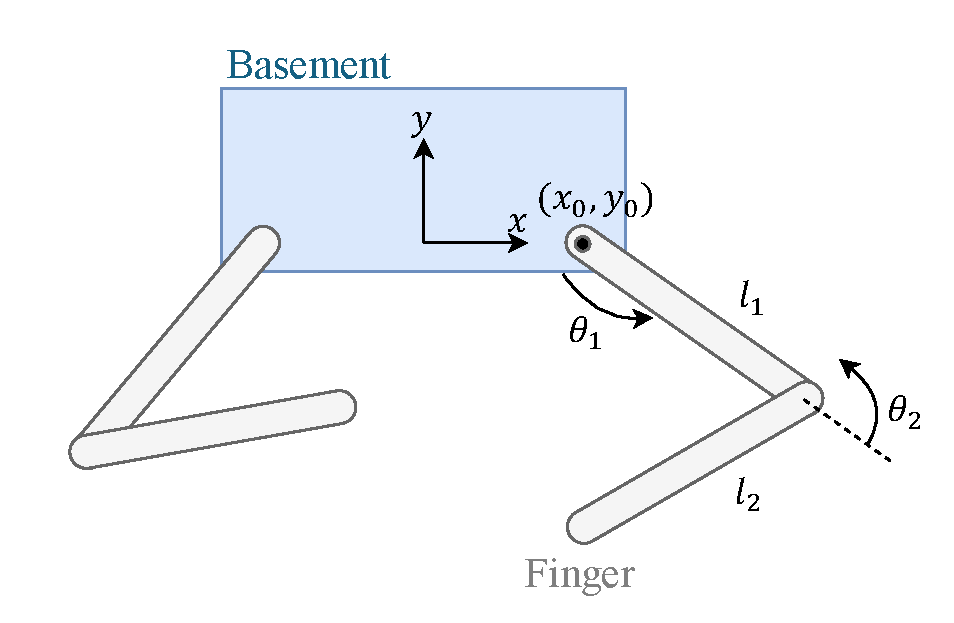
\includegraphics[width=0.8\linewidth]{img/system_kinematics.pdf}  % Replace with your file name
	\caption{The kinematics of the smart grapple system. }
	\label{fig:grapple_kinematics}
\end{figure}
\bds{best make sure to refer to Figure 21 in the main text too} %\ian{add it in previous paragraph.}

The kinematic parameters of the smart grapple system are summarized in \cref{tab:grapple_kinematics} in the appendix. These parameters define the physical dimensions and reference configuration of each finger, which serve as the foundation for the motion planning and grasp control algorithms described in subsequent sections.

\subsubsection{Iteration Solution} \label{sec:IK_iter}
To address the inverse kinematics problem of a multi-link manipulator, the \gls{FABRIK} (Forward And Backward Reaching Inverse Kinematics) algorithm \cite{Aristidou:2011:FABRIK} provides an efficient and intuitive iterative solution. Unlike traditional Jacobian-based or trigonometric approaches, \gls{FABRIK} determines joint positions geometrically by locating each joint along a line connecting its neighboring joints. This geometric interpretation eliminates the need for matrix inversion or complex angle computations, resulting in a low computational cost and fast convergence, typically within only a few iterations.

The algorithm operates through a two-phase iterative process: a forward reaching step and a backward reaching step. In the forward phase, the computation begins from the end effector and sequentially updates each preceding joint position while maintaining the link length constraints, gradually bringing the chain closer to the target. In the backward phase, the process starts from the base joint and propagates the corrections forward again, ensuring that both the end effector and the base maintain their respective positions. Each full forward–backward iteration minimizes the positional error between the end effector and the desired target in Cartesian space.

Assume $\mathbf{p}_1,...,\mathbf{p}_n$ are the joint positions of a manipulator. Also, assume that $\mathbf{p}_1$ is the root joint and $\mathbf{p}_n$ is the end effector, for the simple case where only a single end effector exists. The target is symbolised as t and the initial base
position by b. \gls{FABRIK} is illustrated in pseudo-code in \cref{alg:fabrik} and a graphical representation of a full iteration with a single target and 4 joints is presented and explained in Figure~\ref{fig:fabrik_process}.
\bds{Before Figure was used instead of Fig.} %\ian{This is fixed.}

\gls{FABRIK} is particularly suitable for robotic applications that require fast and stable inverse kinematics computation. It naturally accommodates joint and positional constraints and can be extended to handle multiple kinematic chains with multiple end effectors. Owing to its numerical stability, low computational demand, and realistic motion generation, the \gls{FABRIK} algorithm is an effective choice for solving the inverse kinematics problem of the smart grapple finger system. 

Since the underwater environment is inherently complex and dynamic, the target object may experience motion due to external disturbances. Therefore, the robustness of the \gls{FABRIK} algorithm is crucial. To evaluate its performance within our system, we simulate several scenarios in which the target positions are shifted to mimic the influence of environmental factors, requiring the manipulator fingers to continuously track the actual target location. As illustrated in Figure~\ref{fig:fabrik_sim}, the robot’s arms successfully follow the moving object in real time. When the object moves beyond the manipulator’s reachable workspace under the current constraints, the system automatically issues a warning, indicating that the robot must reposition itself to re-establish reachability and resume grasping.

\begin{algorithm} 
\caption{A full iteration of the \gls{FABRIK} algorithm \cite{Aristidou:2011:FABRIK}}
\label{alg:fabrik}
\begin{algorithmic}[1] 
\State \textbf{Input:} The joint positions $\mathbf{p}_i$ for $i = 1,\ldots,n$, 
the target position $\mathbf{t}$, and the distances between each joint 
$d_i = \lVert \mathbf{p}_{i+1} - \mathbf{p}_i \rVert$ for $i = 1,\ldots,n-1$.
\State \textbf{Output:} The new joint positions $\mathbf{p}_i$ for $i = 1,\ldots,n$.

\Statex
\State \% The distance between root and target
\State $\text{dist} = \lVert \mathbf{p}_1 - \mathbf{t} \rVert$
\State \% Check whether the target is within reach
\If{$\text{dist} > d_1 + d_2 + \ldots + d_{n-1}$}
    \State \% The target is unreachable
    \For{$i = 1,\ldots,n-1$}
        \State \% Find the distance $r_i$ between the target $\mathbf{t}$ and the joint $\mathbf{p}_i$
        \State $r_i = \lVert \mathbf{t} - \mathbf{p}_i \rVert$, $\lambda_i = d_i / r_i$
        \State \% Find the new joint positions $\mathbf{p}_i$
        \State $\mathbf{p}_{i+1} = (1 - \lambda_i)\mathbf{p}_i + \lambda_i \mathbf{t}$
    \EndFor
\Else
    \State \% The target is reachable; thus, set as $\mathbf{b}$ the initial position of the joint $\mathbf{p}_1$
    \State $\mathbf{b} = \mathbf{p}_1$
    \State \% Check whether the distance between the end effector $\mathbf{p}_n$ and the target $\mathbf{t}$ is greater than a tolerance
    \State $\text{difA} = \lVert \mathbf{p}_n - \mathbf{t} \rVert$
    \While{$\text{difA} > \text{tol}$}
        \State \% \textbf{Stage 1: Forward reaching}
        \State \% Set the end effector $\mathbf{p}_n$ as the target $\mathbf{t}$
        \State $\mathbf{p}_n = \mathbf{t}$
        \For{$i = n-1,\ldots,1$}
            \State \% Find the distance $r_i$ between $\mathbf{p}_{i+1}$ and $\mathbf{p}_i$
            \State $r_i = \lVert \mathbf{p}_{i+1} - \mathbf{p}_i \rVert$, $\lambda_i = d_i / r_i$
            \State \% Find the new joint positions $\mathbf{p}_i$
            \State $\mathbf{p}_i = (1 - \lambda_i)\mathbf{p}_{i+1} + \lambda_i \mathbf{p}_i$
        \EndFor

        \State \% \textbf{Stage 2: Backward reaching}
        \State \% Set the root $\mathbf{p}_1$ to its initial position
        \State $\mathbf{p}_1 = \mathbf{b}$
        \For{$i = 1,\ldots,n-1$}
            \State \% Find the distance $r_i$ between $\mathbf{p}_i$ and $\mathbf{p}_{i+1}$
            \State $r_i = \lVert \mathbf{p}_{i+1} - \mathbf{p}_i \rVert$, $\lambda_i = d_i / r_i$
            \State \% Find the new joint positions $\mathbf{p}_{i+1}$
            \State $\mathbf{p}_{i+1} = (1 - \lambda_i)\mathbf{p}_i + \lambda_i \mathbf{p}_{i+1}$
        \EndFor
        \State $\text{difA} = \lVert \mathbf{p}_n - \mathbf{t} \rVert$
    \EndWhile
\EndIf

\end{algorithmic}
\end{algorithm}

\begin{figure}[!htbp]
    \centering
    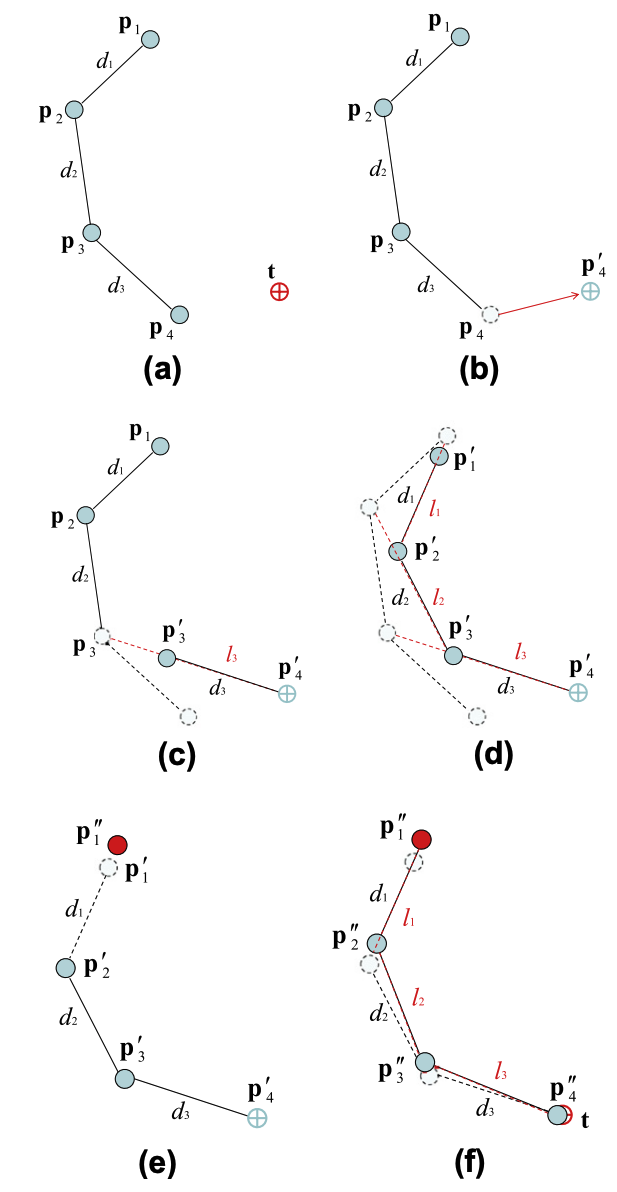
\includegraphics[width=0.5\linewidth]{img/fabrik_process.png}  % Replace with your file name
	\caption{\cite{Aristidou:2011:FABRIK} Illustration of one full iteration of the \gls{FABRIK} algorithm for a manipulator with four joints and a single target. (a) Initial configuration of the manipulator and target; (b) the end-effector $\mathbf{p}_4$ is moved to the target position; (c) the new joint position $\mathbf{p}_3'$ is computed along the line $l_3$ connecting $\mathbf{p}_4'$ and $\mathbf{p}_3$, maintaining the distance $d_3$ from $\mathbf{p}_4'$; (d) the same procedure is applied sequentially to the remaining joints; (e) in the backward stage, the root joint $\mathbf{p}_1'$ is moved back to its original position; (f) the process is repeated from the base toward the end-effector. The iteration continues until the end-effector reaches or sufficiently approaches the target. }
	\label{fig:fabrik_process}
\end{figure}

\begin{figure}[!htbp]
    \centering
    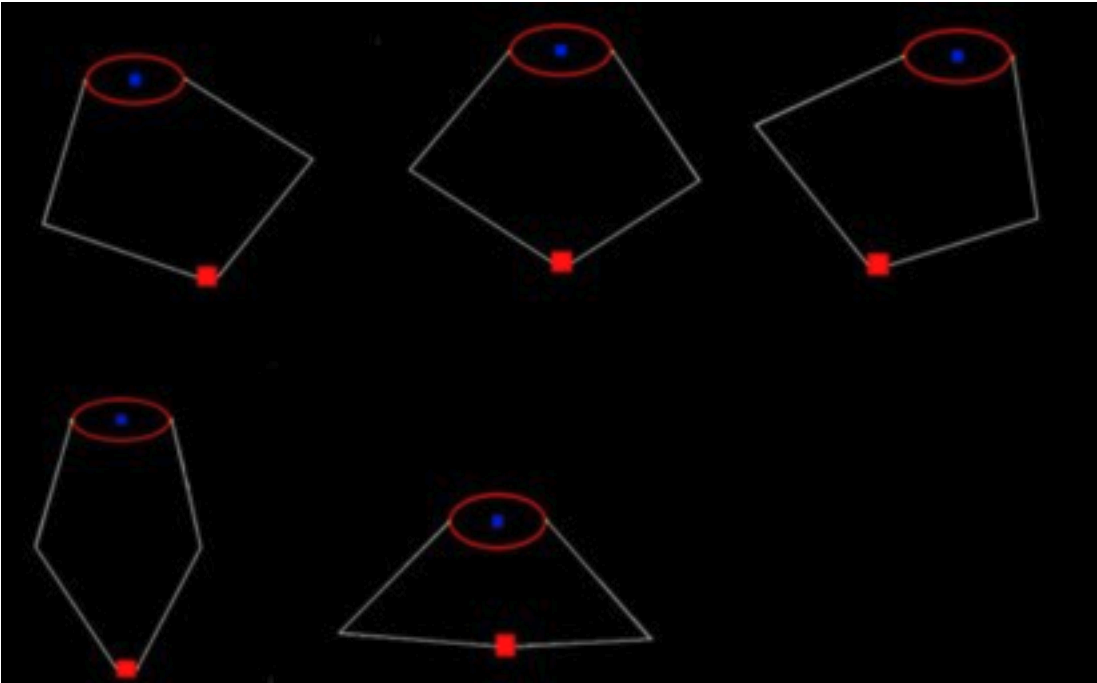
\includegraphics[width=0.7\linewidth]{img/fabrik_simulation.png}  % Replace with your file name
	\caption{\gls{FABRIK} reacting to target movement. The red square symbolizes the robot's
body. Blue square symbolizes the target base point. The red ellipse visualizes the
target's shape. Gray lines visualize the robot arms. }
	\label{fig:fabrik_sim}
\end{figure}

\subsection{Optimal Grasping Manipulability Under Joint Position and Joint Torque Constraints}\label{optimal-grasping}

To ensure that the smart grapple can securely lift underwater litter, it must generate sufficient force to counteract the object’s weight while maintaining a reliable frictional interface. Consider a litter object of mass $M$, with friction coefficient $\mu$, gravitational acceleration $g$, and end-effector force components $(F_x, F_y)$. The static equilibrium of the object requires
\begin{equation}
    Mg = \mu F_x + F_y,
\end{equation}
where $\mu$ corresponds to the surface properties of different debris types, summarized in \cref{tab:friction_coeff}.

\begin{table}[h!]
\centering
\caption{Friction coefficients of common litter objects.}
\label{tab:friction_coeff}
\begin{tabular}{l c}
\hline
\textbf{Object Type} & \textbf{Friction Coefficient} \\
\hline
Barrel         & 0.60  \\
E-scooter      & 0.60  \\
Steel pipe     & 0.60  \\
Tractor tire   & 0.86  \\
Car tire       & 0.86  \\
\hline
\end{tabular}
\end{table}

\subsubsection{Grasping Scenarios}   \label{sec:percentageControlImplementation}
In practice, the available perception information varies depending on environmental conditions. Therefore, three grasping scenarios are considered, as illustrated in Figure~\ref{fig:graps_scene}. These scenarios differ in flexibility, force performance, and dependence on vertical control.  \bds{what are in practice these scenarios and when do we encounter them?} %\ian{I explain which case we use in practice in the  paragraph below.}

\begin{itemize}
    \item \textbf{Case 1: Full Cartesian Control.}  
    The desired end-effector position is directly commanded through the joint space. This offers maximum grasping flexibility but does not necessarily maximize force output.
    \item \textbf{Case 2: Force-Optimized Grasping.}  
    The vertical grasping position is optimized with respect to object width to maximize the attainable horizontal force. This enables the system to exploit the full manipulability of the finger mechanism.
    \item \textbf{Case 3: Fixed Optimal Height for Multi-Width Objects.}
    A single, globally optimal vertical height is selected, enabling robust grasping performance across various object widths while simplifying underwater motion planning.
\end{itemize}

\ian{In practice, since we need to compromise the flexibility and force performance, we consider the case 3 in the sea trial.}

\begin{figure}[!htbp]
    \centering
    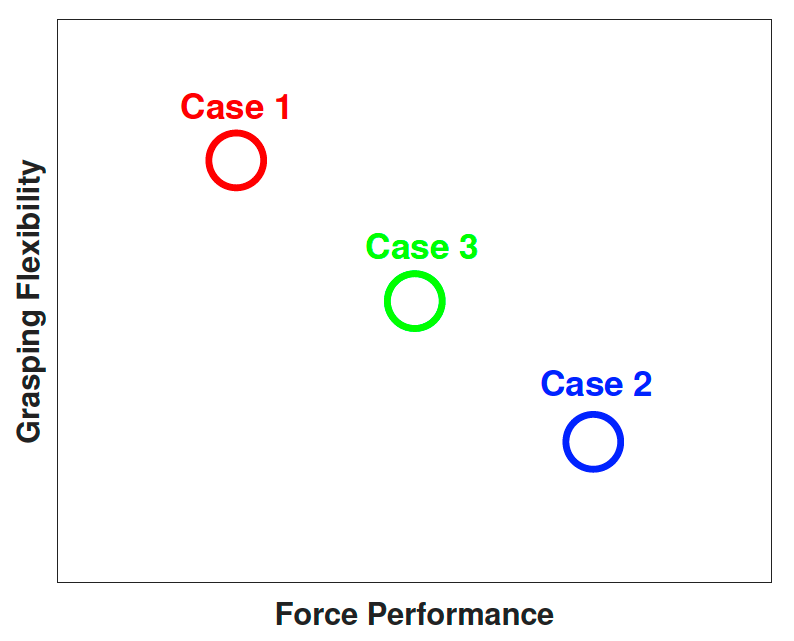
\includegraphics[width=0.39\linewidth]{img/grasping_3case.png}
    \caption{Comparison of grasping flexibility and force performance across the three scenarios.}
    \label{fig:graps_scene}
\end{figure}

\subsubsection{Static Force Analysis}

To describe the static relationship between joint torques and end-effector forces, we apply the principle of virtual work. Let $W$ denote virtual work and $P$ denote power. For the two-joint finger mechanism, the work and power on the joint side are
\begin{equation}
    W = \tau_1\, \delta\theta_1 + \tau_2\, \delta\theta_2, \label{eq:v_work}
\end{equation}
\begin{equation}
    P = \tau_1 \dot{\theta}_1 + \tau_2 \dot{\theta}_2 = \dot{\boldsymbol{\theta}}^{\,T} \vec{\tau}. \label{eq:power}
\end{equation}

On the end-effector side, the corresponding expressions are
\begin{equation}
    W = \delta x \cdot F, \label{eq:out_work}
\end{equation}
\begin{equation}
    P = v \cdot F = (J(\boldsymbol{\theta})\dot{\boldsymbol{\theta}})^T F
      = \dot{\boldsymbol{\theta}}^{\,T} J(\boldsymbol{\theta})^T F, \label{eq:out_power}
\end{equation}
where $J(\boldsymbol{\theta})$ is the Jacobian matrix of the finger, given by
\begin{equation} \label{eq:jacobian}
J(\boldsymbol{\theta}) =
\begin{bmatrix}
 l_1 \sin\theta_1 + l_2 \sin(\theta_1+\theta_2) & l_2 \sin(\theta_1+\theta_2) \\
 -l_1 \cos\theta_1 - l_2 \cos(\theta_1+\theta_2) & -l_2 \cos(\theta_1+\theta_2)
\end{bmatrix}.
\end{equation}

Equating the power expressions in \eqref{eq:power} and \eqref{eq:out_power}, we obtain the fundamental static relationship:
\begin{equation}
    \vec{\tau} = J(\boldsymbol{\theta})^T F.
\end{equation}

Provided that $J(\boldsymbol{\theta})$ is invertible, the end-effector force can be computed from the joint torques as
\begin{equation}
\begin{bmatrix}
F_x \\ F_y
\end{bmatrix}
=
(J(\boldsymbol{\theta})^T)^{-1} \vec{\tau}.
\end{equation}

Explicitly, this yields
\begin{equation}
F_x = \frac{\cos\theta_1}{l_2 \sin\theta_2}\, \vec{\tau},
\label{eq:Fx}
\end{equation}
\begin{equation}
F_y = \frac{\sin\theta_1}{l_2 \sin\theta_2}\, \vec{\tau}.
\label{eq:Fy}
\end{equation}

A singular configuration arises when $\det(J(\boldsymbol{\theta})) = 0$, resulting in loss of controllability and unbounded joint torques. From \eqref{eq:jacobian}, the determinant is
\begin{equation}
    \det(J(\boldsymbol{\theta})) = l_1 l_2 \sin(\theta_2).
\end{equation}

Thus, singularity occurs when $\theta_2 = 0$ or $\theta_2 = \pi$. To avoid these conditions, we construct a $5$~cm band around the singular boundary, defining the \emph{safe workspace} shown in Figure~\ref{fig:safe_workspace}.

\begin{figure}[!htbp]
    \centering
    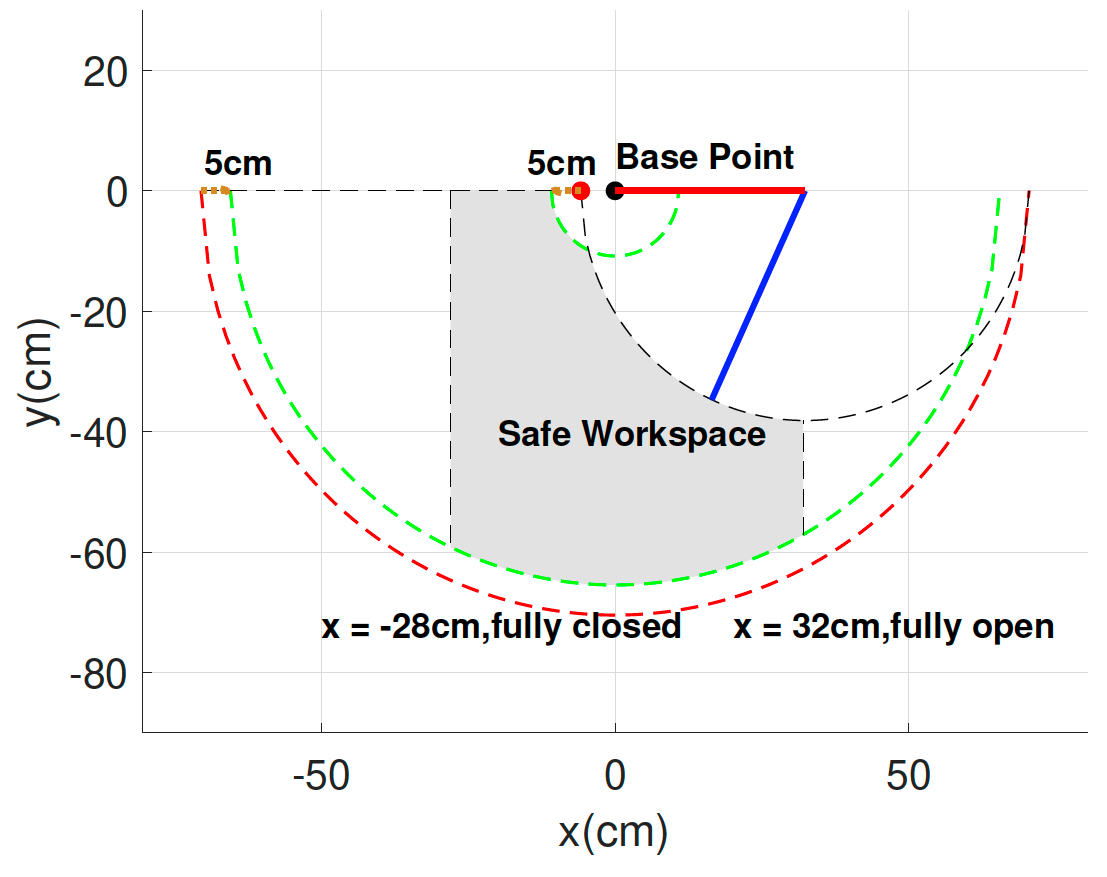
\includegraphics[width=0.59\linewidth]{img/singular_circle_grasp.png}
    \caption{The safe workspace for a single finger after excluding a 5~cm neighborhood of singular configurations.}
    \label{fig:safe_workspace}
\end{figure}

\subsubsection{Grasping Posture in Different Scenarios}

To determine an appropriate grasping posture across different operational scenarios, we develop a unified framework for computing the joint commands associated with each case. In all scenarios, we assume that the \emph{horizontal} target position (i.e., the object width) is obtained from the perception system. Depending on the level of available information, we consider three distinct cases.

\paragraph{Case 1: Full Target Position Known.}
In this case, both the horizontal and vertical target positions of the end effector are given. Thus, the complete Cartesian target $(x^{*},y^{*})$ is available. The corresponding joint configuration can be computed using either the analytical inverse kinematics method introduced in \cref{sec:IK_ana} or the iterative FABRIK method described in \cref{sec:IK_iter}. Once the joint angles are obtained, the grasping forces can be evaluated using \eqref{eq:Fx} and \eqref{eq:Fy}. The resulting force distribution within the safe workspace is illustrated in Figure~\ref{fig:fx_dis}.

\begin{figure}[!htbp]
    \centering
    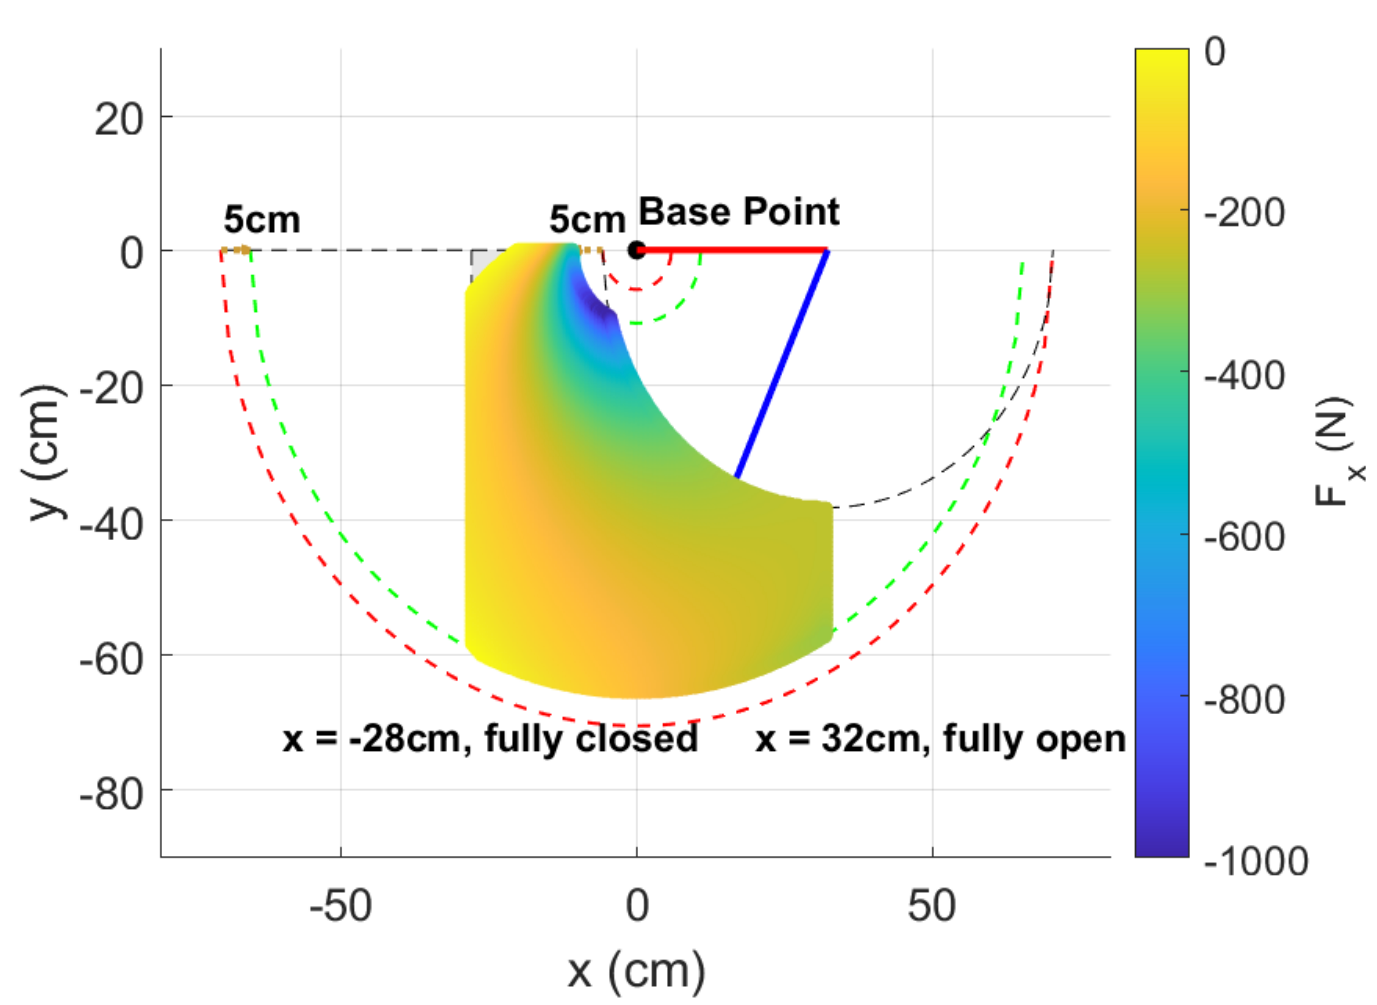
\includegraphics[width=0.59\linewidth]{img/fx_distribuion.png}  % Replace with your file name
	\caption{The force distribution in the safe workspace.}
	\label{fig:fx_dis}
\end{figure}

\paragraph{Case 2: Horizontal Position Known, Vertical Position to be Optimized.}
When only the horizontal target position is known, i.e., $x^{*}\in\mathcal{X}$ where $\mathcal{X}$ denotes the admissible horizontal workspace, the vertical position must be selected so as to maximize the achievable horizontal gripping force. Formally, the optimal vertical position is obtained by

\begin{equation}
    y^{*}=\argmax_{y\in\mathcal{Y}}\, F_{x}(x^{*},y),
\end{equation}

where $\mathcal{Y}$ is the feasible vertical workspace. The value $y^{*}$ is computed using an optimization toolbox, after which the associated joint configuration can be determined via inverse kinematics. By evaluating the optimizer over all feasible object widths, we obtain a mapping from $x^{*}$ to the corresponding optimal vertical position, which is illustrated in Figure~\ref{fig:opt_vertical_traj}, and the joint configuration that maximizes the horizontal force within the safe workspace.

\begin{figure}[!htbp]
    \centering
    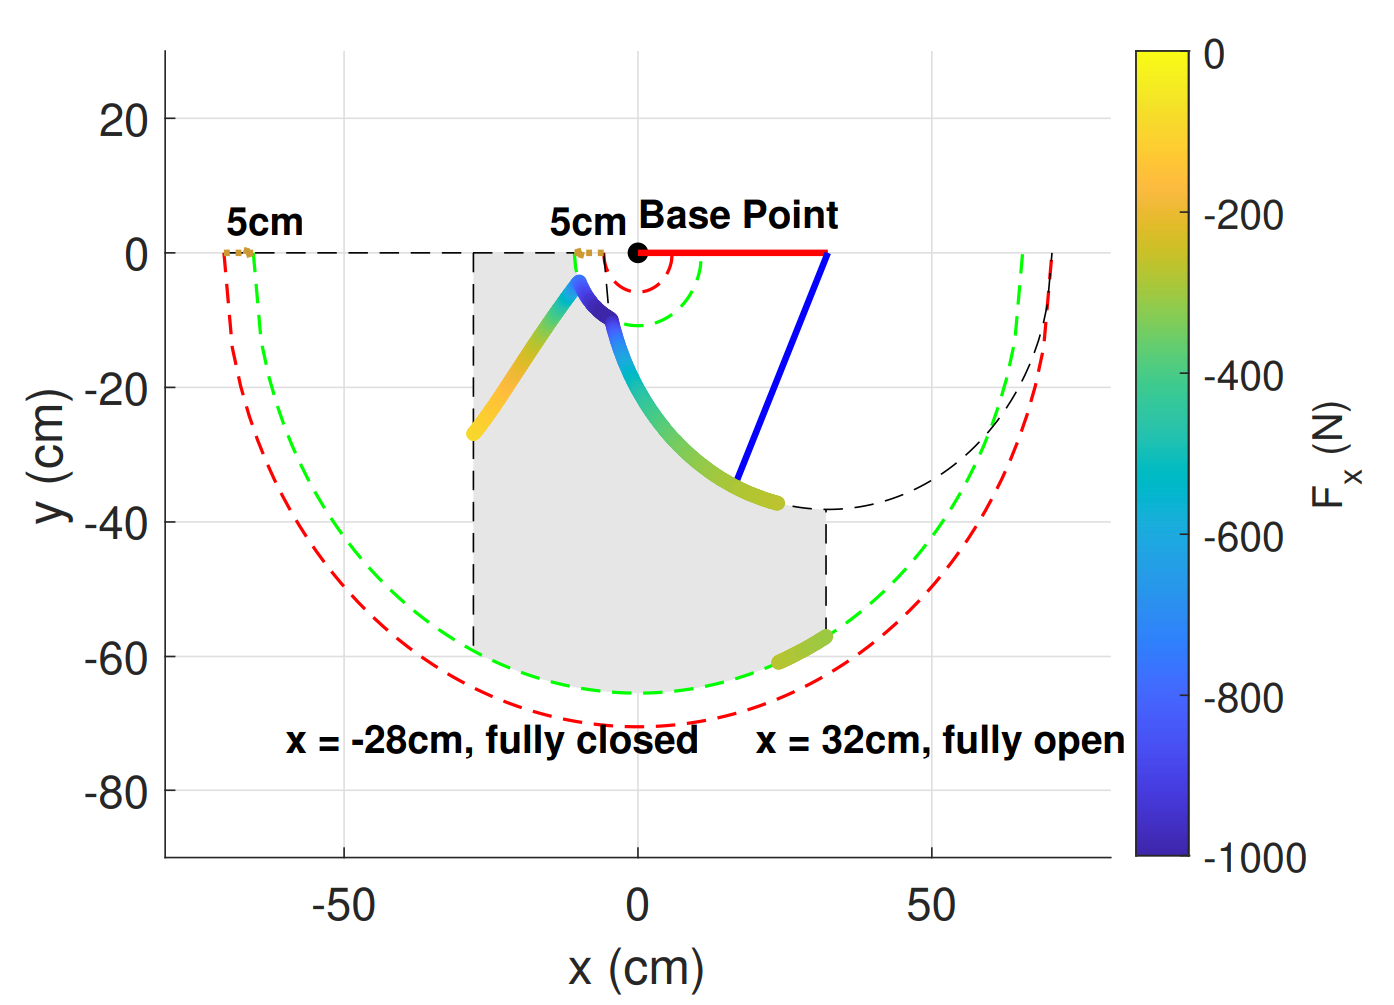
\includegraphics[width=0.59\linewidth]{img/opt_y_case2.png}  % Replace with your file name
	\caption{The optimized vertical position trajectory.}
	\label{fig:opt_vertical_traj}
\end{figure}

\paragraph{Case 3: Fixed Grasping Position with Good Average Performance.}
Although Case~2 yields the force-maximizing posture for each object width, the resulting optimal vertical position $y^{*}$ varies with the target. Consequently, the smart grapple would need to continuously adjust its vertical position, which is challenging in underwater environments due to hydrodynamic disturbances and limited maneuverability. To avoid frequent repositioning, we instead seek a \emph{single} vertical position that provides consistently good average performance across different object widths.

To achieve this, let \ian{$(x_j, y_i)$} %\bds{I would recommend to use round brackets here (representing a pair) instead of curly brackets (representing a set), or else use $\{(x_i,y_i)\}_{i}$.} represent sampled points in the safe workspace $\mathcal{X}\times\mathcal{Y}$. For each vertical position $y_i$, we compute the corresponding horizontal force $F_x^j(y_i)$ over all sampled widths $x_j$. We then compute the mean force and its variance at level $y_i$:
\[
    \bar{F}_x^{\,i} = \frac{1}{|\mathcal{X}|}\sum_{j} F_x^j(y_i), 
    \qquad
    \sigma_i^2 = \frac{1}{|\mathcal{X}|}\sum_{j} \left(F_x^j(y_i)-\bar{F}_x^{\,i}\right)^2.
\]
The optimal vertical posture is obtained by balancing high average performance and low variability, expressed as

\begin{equation}
    y^{*} = \argmax_{y_i\in\mathcal{Y}} \; \Phi(\,\bar{F}_x^{\,i},\,\sigma_i\,),
\end{equation}

where $\Phi(\cdot)$ denotes a performance metric that rewards larger average force while penalizing high variance. This yields a robust grasping posture that performs well across a range of object widths without requiring vertical repositioning of the smart grapple.

\subsection{Gripping points optimization} \label{sec:Gripping_points_opt}
As presented in Subsection \ref{optimal-grasping}, there might be several possible grasping configurations for a given object, some of them being optimal under selected criteria. However, these criteria cannot be complete, unless the shape and size of the object is also taken into consideration. The object detection component presented in Section \ref{sec:static_tsdf} is providing a point cloud of the litter that needs to be picked. As a next step to the gripping pipeline, we have developed a ROS2 service, that consumes this point cloud and is then reconstructing a surface mesh based on it. Surfaces that are not suitable for gripping (e.g. horizontal surfaces) are then filtered out. An optimization routine is checking all possible pairs of opposite gripping surfaces (for two fingers), and for each pair it checks all kinematically possible surfaces for the other two fingers. For each quadruplet of surfaces, it calculates the forces that the grapple can exert on them, and eventually picks the quadruplet that can be grasped with maximal forces. This ensures that the grapple will pick the object in the most favourable configuration, therefore increasing the chances of a successful litter picking. The procedure for the gripping points optimization is presented graphically in Figure~\ref{fig:gripping_service}. This gripping points optimization was done in the SeaGrip project, supported by a grant of the Ministry of Research, Innovation and Digitization, CNCS/CCCDI -UEFISCDI, project number PN-IV-P8-8.1-PRE-HE-ORG-2023-0012, within PNCDI IV. The project results were later integrated in the SeaClear2.0 grasping pipeline. \bds{is the work in the aforementioned project separate to the SC2 and we simply use the research outcomes? if yes, then better reference the project itself, rather than the funding organisation. If not, formulate the text in such way that cross-funding can be ruled out.}

\begin{figure}[phtb]
    \centering
    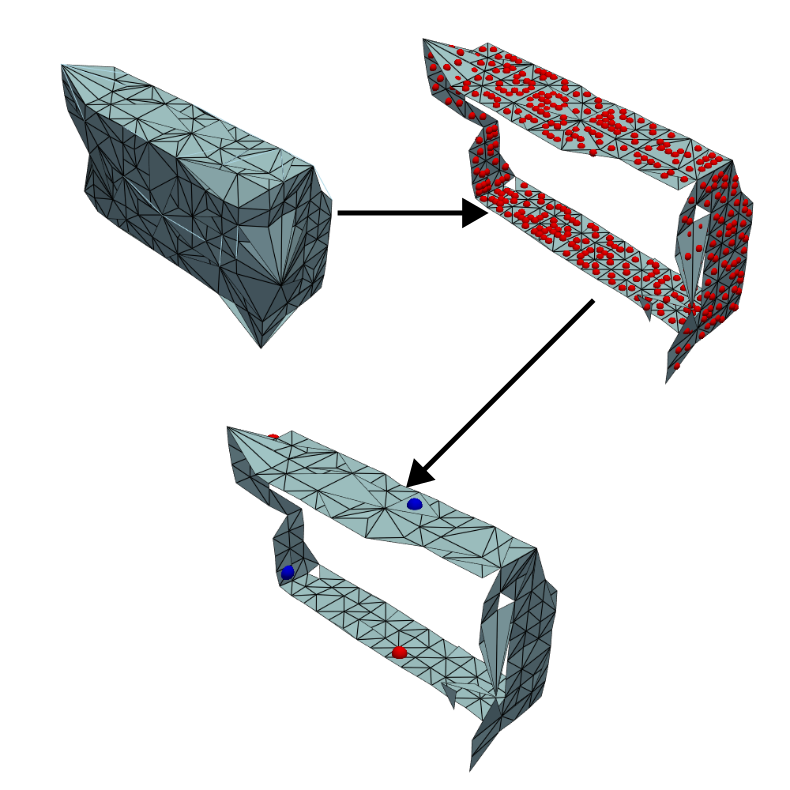
\includegraphics[width=0.7\linewidth]{img/vision_pipeline/gripping_service.png}
    \caption{Steps of the gripping points service. We first reconstruct a mesh based on the point cloud provided by the object detection algorithm. The surfaces appropriate for grasping are then isolated, and the service is calculating the optimal surfaces for gripping based on force analysis of the grapple.}
    \label{fig:gripping_service}
\end{figure}

%%%%%%%%%%%%%%%%%%%%%%%%%%%%%%%%%%%%%%%%%%%%%%%%
% Section break
\section{Digital Twin of the Smart Grapple}
\label{sec:sim}
Due to the scarce availability of sea trials, the \gls{usg} is mostly tested in the lab. Additionally, a simulation-based, digital twin approach is used to validate the system between field tests.

Simulation is conducted using the \gls{marus} tool. The source code of the \gls{usg} is stored in a separate Docker container from the \gls{marus} interface. This \gls{sil} method helps to bridge the sim-to-real gap by allowing the same source code to run in the real system with minimal changes. It also accelerates development since no extra code is needed for simulation.

\textbf{Scope of the Simulation.}
The digital twin is currently able to reproduce navigation of the \gls{usg}. That means the perception, planning, and tracking sub-modules are already integrated in the simulation pipeline. Figure~\ref{fig:simPipe} visualizes the software stack for simulation and Figure~\ref{fig:simGameView} shows the digital twin in the virtual environment. 

\begin{figure}[ht]
	\centering
	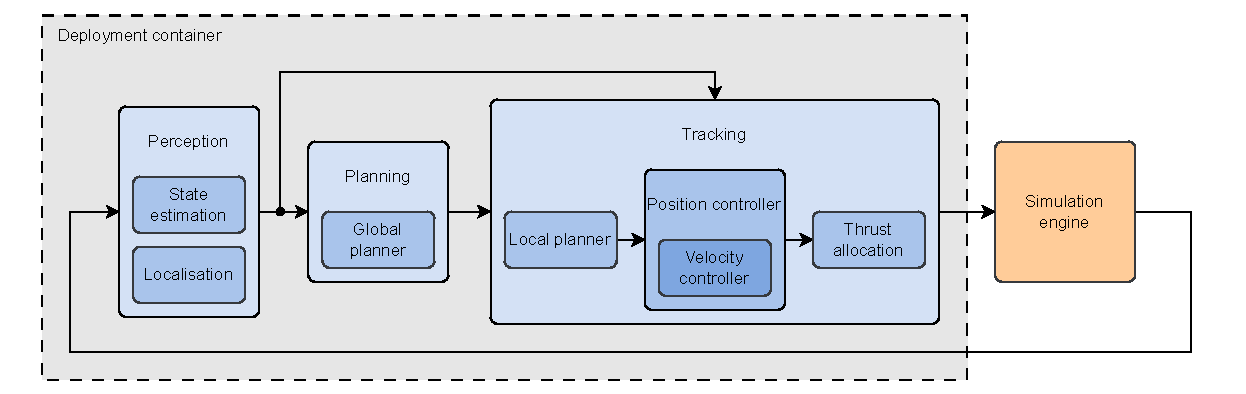
\includegraphics[width=\textwidth]{img/tracking_software_stack.drawio.pdf}
	\caption{Software stack of the simulation pipeline}
	\label{fig:simPipe}
\end{figure}

\textbf{MARUS Engine.}
The \gls{marus} simulation engine was developed by the \textit{Laboratory for Underwater Systems and Technologies} at the University of Zagreb \cite{9976969}. It is an open-source simulator for marine robotics based on the Unity3D software. The main benefits of this simulator are:
\begin{itemize}
    \item Native ROS 2 support,
    \item Realistic underwater visual data (needed for machine learning computer vision algorithms),
    \item Availability of standard sensors in marine robotics, such as \gls{dvl}, depth sensor, sonar, and acoustic communication,
    \item Mesh-based approximation of hydrodynamics,
    \item Ongoing development.
\end{itemize}

\begin{figure}[ht]
	\centering
	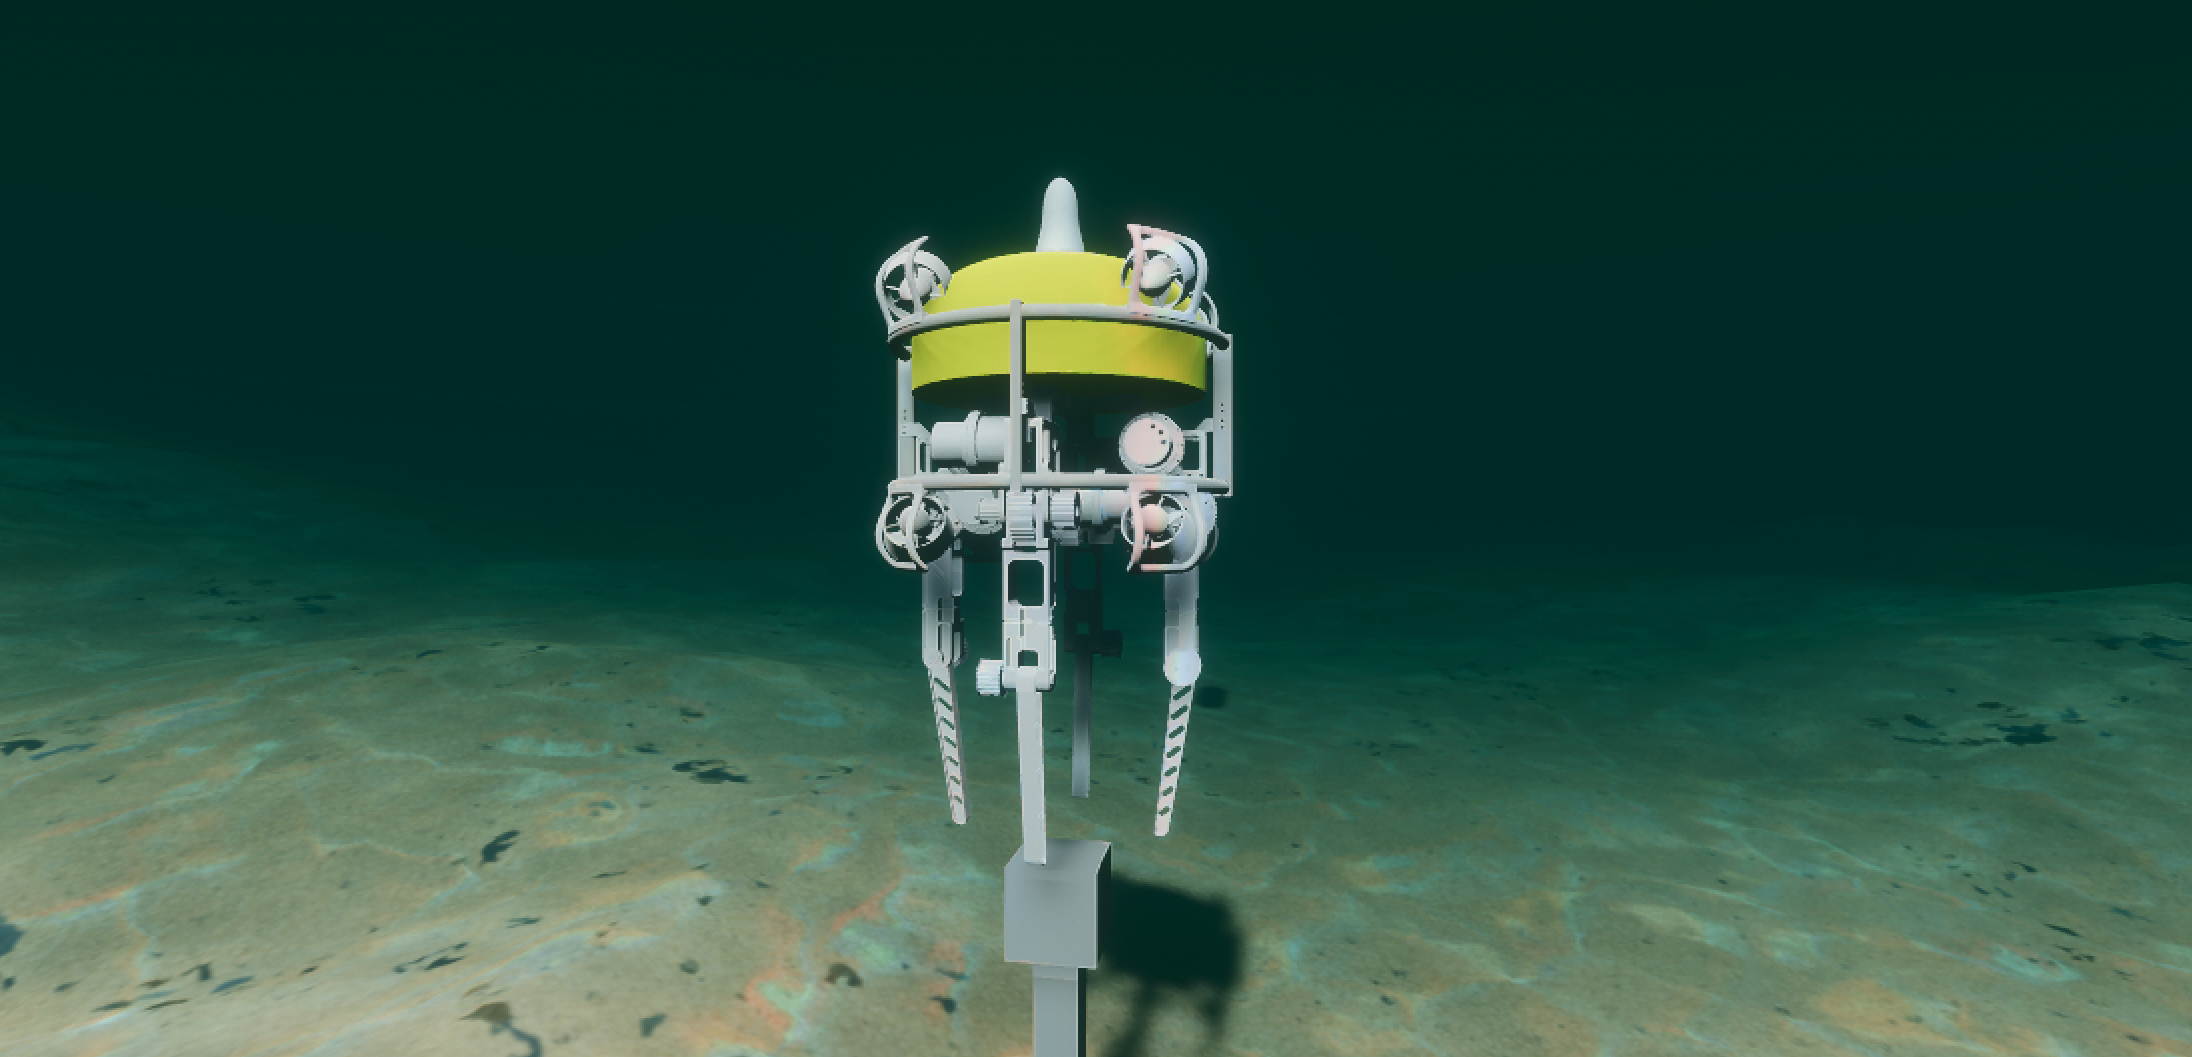
\includegraphics[width=\textwidth]{img/unity_sim_game_view.png}
	\caption{Digital twin in the virtual environment}
	\label{fig:simGameView}
\end{figure}
%%%%%%%%%%%%%%%%%%%%%%%%%%%%%%%%%%%%%%%%%%%%%%%%

\section{Experiments}

This section presents the experimental validation of the Smart Grapple system through both controlled laboratory tests and field demonstrations. Laboratory experiments systematically evaluated the grapple's load-bearing capacity by progressively grasping objects up to 251~kg, recording joint positions and torques at each weight increment to verify that the system meets the 250~kg design requirement. Field results from the Marseille demonstration in September 2025 provide real-world validation, documenting successful retrieval of various marine litter objects including a car seat, tire, fences, and an attempted grasp of a shipwreck fragment, with detailed analysis of sensor outputs during representative grasping maneuvers.

\subsection{Laboratory tests}
To validate that the grapple can securely grasp objects up to 250 kg, a series of experiments was conducted in which weights were progressively added to a test container until the total load exceeded 250 kg. For each trial, the grapple was lifted up with the container vertically, replicating the operational conditions encountered during underwater litter retrieval. The stability of the grasp was evaluated by verifying whether the object remained securely held throughout the lifting motion. All tested weights were successfully grasped, and the results are summarized in \cref{tab:exp_grasp_weight}. These experiments demonstrate that the system is capable of reliably handling objects ranging up to 250 kg, as shown in Figure~\ref{fig:grasp_250_test}. 

\begin{figure}
    \centering
    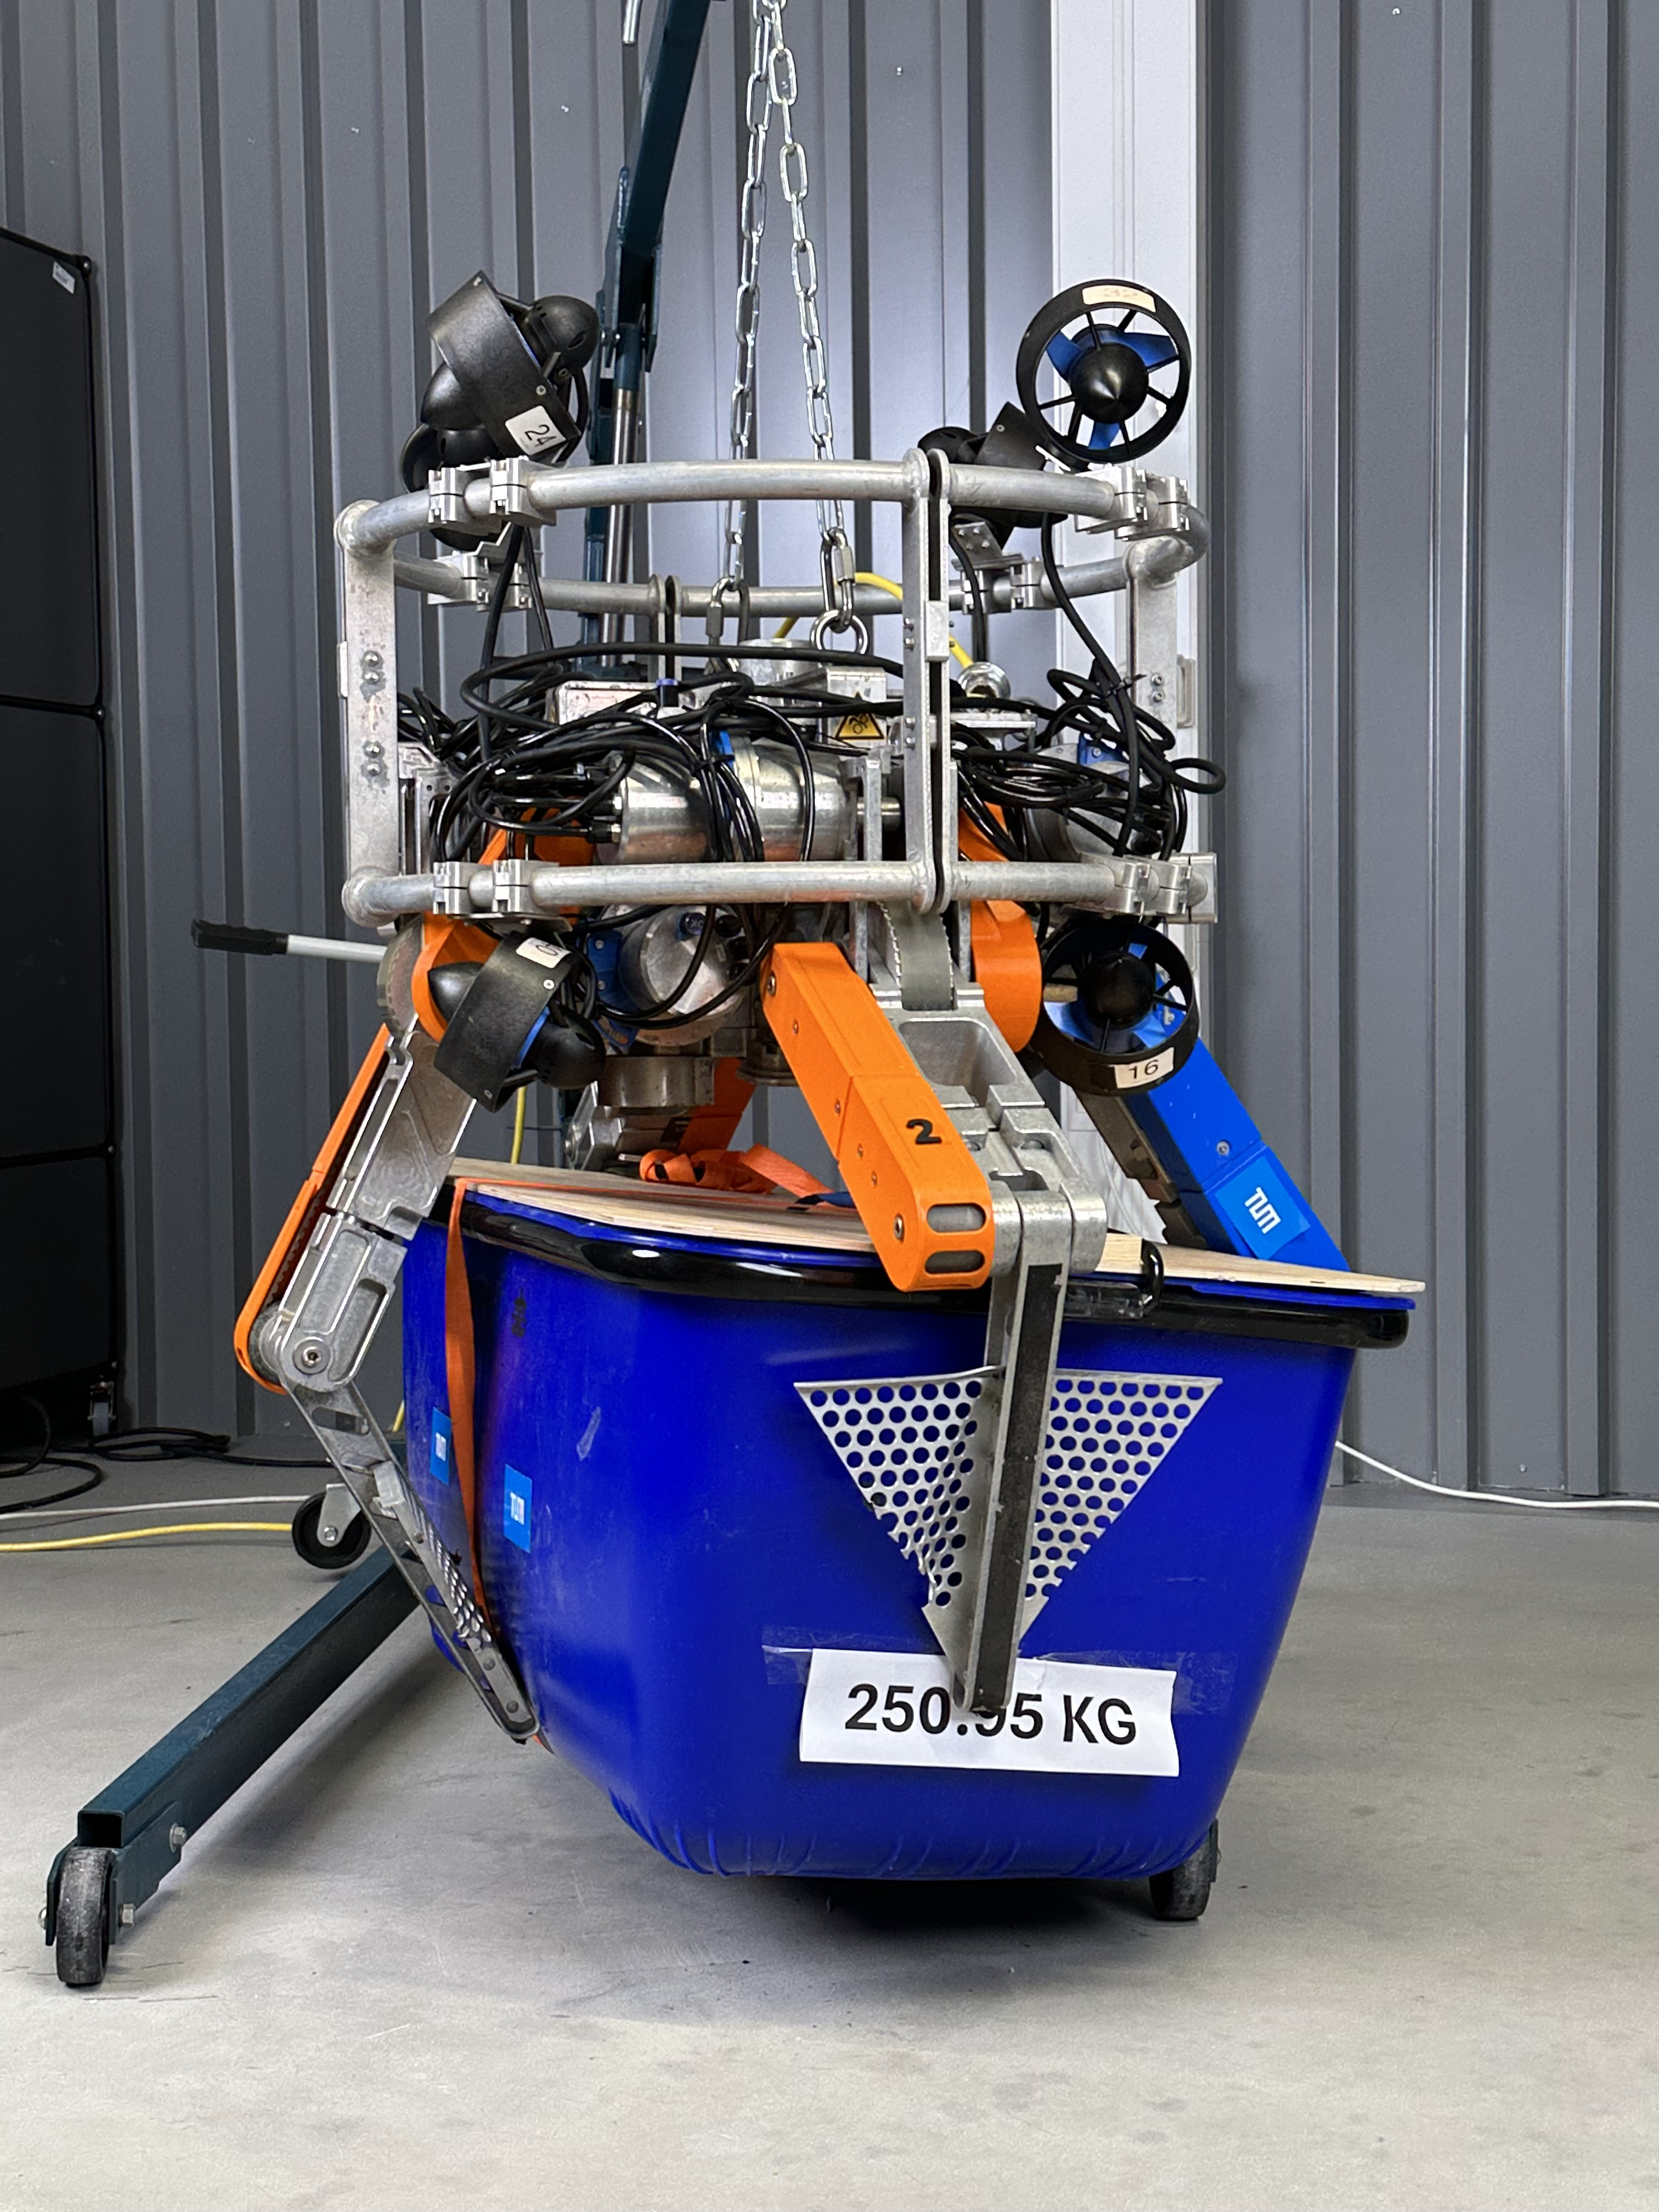
\includegraphics[width=0.5\linewidth]{img/grasp_250kg_test.jpeg}
    \caption{The smart grapple lifting a box of 250 kg under controlled conditions.}
    \label{fig:grasp_250_test}
\end{figure}

\begin{table}[htbp]
\centering
\small
\renewcommand{\arraystretch}{1.1}
\setlength{\tabcolsep}{3pt}
\caption{Joint position and torque values for different object weights.}
\begin{tabular}{|c|p{7cm}|p{7cm}|}
\hline
\label{tab:exp_grasp_weight}
\textbf{Weight [kg]} & \textbf{Joint Position [rad]} & \textbf{Joint Torque [Nm]} \\
\hline
20 & (2.72, -1.71, 2.47, -2.28, 2.77, -1.79, 2.47, -2.14) & (5.82, 2.70, 2.88, 18.53, 2.15, 0.73, 7.35, 5.27) \\
\hline
40 & (2.77, -1.79, 2.32, -2.16, 2.77, -1.79, 2.57, -2.04) & (3.14, 5.81, 5.97, 2.68, 3.96, 5.39, 3.76, 3.73) \\
\hline
60 & (2.77, -1.79, 2.32, -2.16, 2.77, -1.79, 2.57, -2.04) & (3.07, 5.81, 6.00, 2.65, 4.00, 5.39, 3.76, 3.73) \\
\hline
80 & (2.77, -1.79, 2.32, -2.16, 2.77, -1.79, 2.57, -2.04) & (3.06, 5.81, 6.02, 3.63, 4.02, 5.87, 3.31, 4.60) \\
\hline
100 & (2.72, -1.81, 2.47, -2.28, 2.77, -1.89, 2.47, -2.24) & (14.18, 27.89, 3.27, 14.61, 2.88, 23.92, 2.62, 15.93) \\
\hline
120 & (2.72, -1.81, 2.47, -2.28, 2.77, -1.89, 2.47, -2.24) & (13.69, 27.71, 3.27, 14.66, 2.49, 23.23, 2.41, 16.02) \\
\hline
140 & (2.72, -1.81, 2.47, -2.28, 2.77, -1.89, 2.47, -2.24) & (12.91, 27.57, 3.01, 14.68, 2.31, 22.99, 2.24, 16.05) \\
\hline
160 & (2.72, -1.81, 2.47, -2.28, 2.77, -1.89, 2.47, -2.24) & (12.94, 27.58, 2.96, 14.95, 3.17, 23.22, 2.88, 16.13) \\
\hline
180 & (2.72, -1.81, 2.47, -2.28, 2.77, -1.89, 2.47, -2.24) & (12.44, 27.49, 3.38, 15.17, 2.96, 23.03, 3.02, 16.43) \\
\hline
194 & (2.81, -2.29, 2.78, -1.89, 2.41, -2.57, 2.77, -1.95) & (3.74, 22.13, 4.31, 13.85, 2.97, 13.54, 6.94, 16.32) \\
\hline
200 & (2.72, -1.81, 2.47, -2.28, 2.77, -1.89, 2.47, -2.24) & (12.71, 27.52, 4.40, 15.48, 3.31, 23.06, 2.98, 16.44) \\
\hline
220 & (2.70, -2.23, 2.87, -1.88, 2.56, -2.53, 2.83, -1.91) & (6.07, 17.19, 4.49, 9.34, 6.73, 10.77, 7.28, 16.56) \\
\hline
251 & (2.55, -1.54, 2.76, -1.61, 2.47, -1.50, 2.76, -1.62) & (11.43, 6.90, 12.74, 11.34, 12.59, 8.90, 16.12, 12.71) \\
\hline
\end{tabular}
\end{table}


\subsection{Field Results in Marseille 2025}
\begin{table}[h!]
\centering
\begin{tabular}{|l|c|c|}
\hline
\textbf{Object} & \textbf{Weight (\gls{usv} Force Sensor Reading)} & \textbf{Dry Weight (Only Object)} \\ \hline
Chair (1)           &      ---                             & 24 kg                                \\ \hline
Tire            &  ---                                  & 6 kg                             \\ \hline
Car Seat         & 185 kg (all together)                  & 45 kg                         \\ \hline
Fences (×2)     & 156 kg (everything / force sensor)     & 14 kg                           \\ \hline
Ship wreck     & 185 kg                   & ---                             \\ \hline
\end{tabular}
\caption{Objects grasped in Marseille with corresponding weights. Dry weight is measured separately outside of the water, if available. The \gls{usv} sensor reading includes the weight of the smart grapple and additional components.\bds{table not referenced in text. Also, why is the weight not estimated using the readings of the force sensors on the USV? Or alternatively, put the torque readings as in the previous table?}} %\ian{the table is referred in the text now, and the weight is estimated by USV here.}
\label{tab:marseille_objects}
\end{table}


\paragraph{Grasping of a car seat and a tire on the media day}
In the following, we analyze selected sensor outputs from the Marseille demo in September 2025. We focus on a representative grasping maneuver of a car seat to verify that the grasping algorithms and hardware components behave as expected. \ian{The result for grapsing object is recorded in \cref{tab:marseille_objects}.} The grasped object is shown in Figure~\ref{fig:grasping_cam}. At the time of grasping, which occurs shortly after \(t \approx 800\,\mathrm{s}\) in the recorded ROS bag, the shoulder joints move from their open to their closed configuration (Figure~\ref{fig:shoulder_positions}), and the elbow joints follow the same pattern (Figure~\ref{fig:elbow_positions}). As soon as the smart grapple closes, the joint torques at all degrees of freedom increase noticeably, again shortly after \(800\,\mathrm{s}\), as illustrated in Figure~\ref{fig:joint_torques}.

\begin{figure}[!h]
    \centering
    %----------------------------------------------------------
    \begin{subfigure}[t]{0.45\textwidth}
        \centering
        % Crop left, bottom, right, top (adjust as needed)
        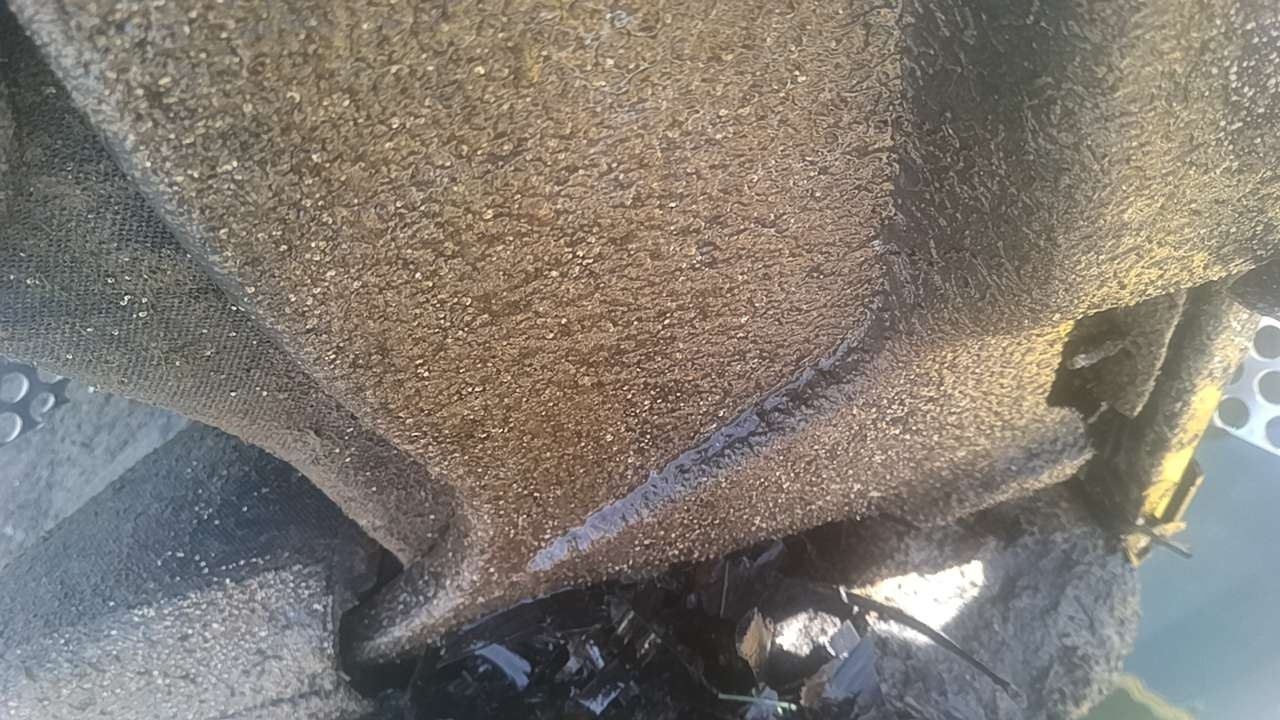
\includegraphics[width=\textwidth]{img/downward_facing camera.png}
        \caption{Grapple view: downward-facing camera.}
        \label{fig:down_cam}
    \end{subfigure}
    \hfill
    %----------------------------------------------------------
    \begin{subfigure}[t]{0.45\textwidth}
        \centering
        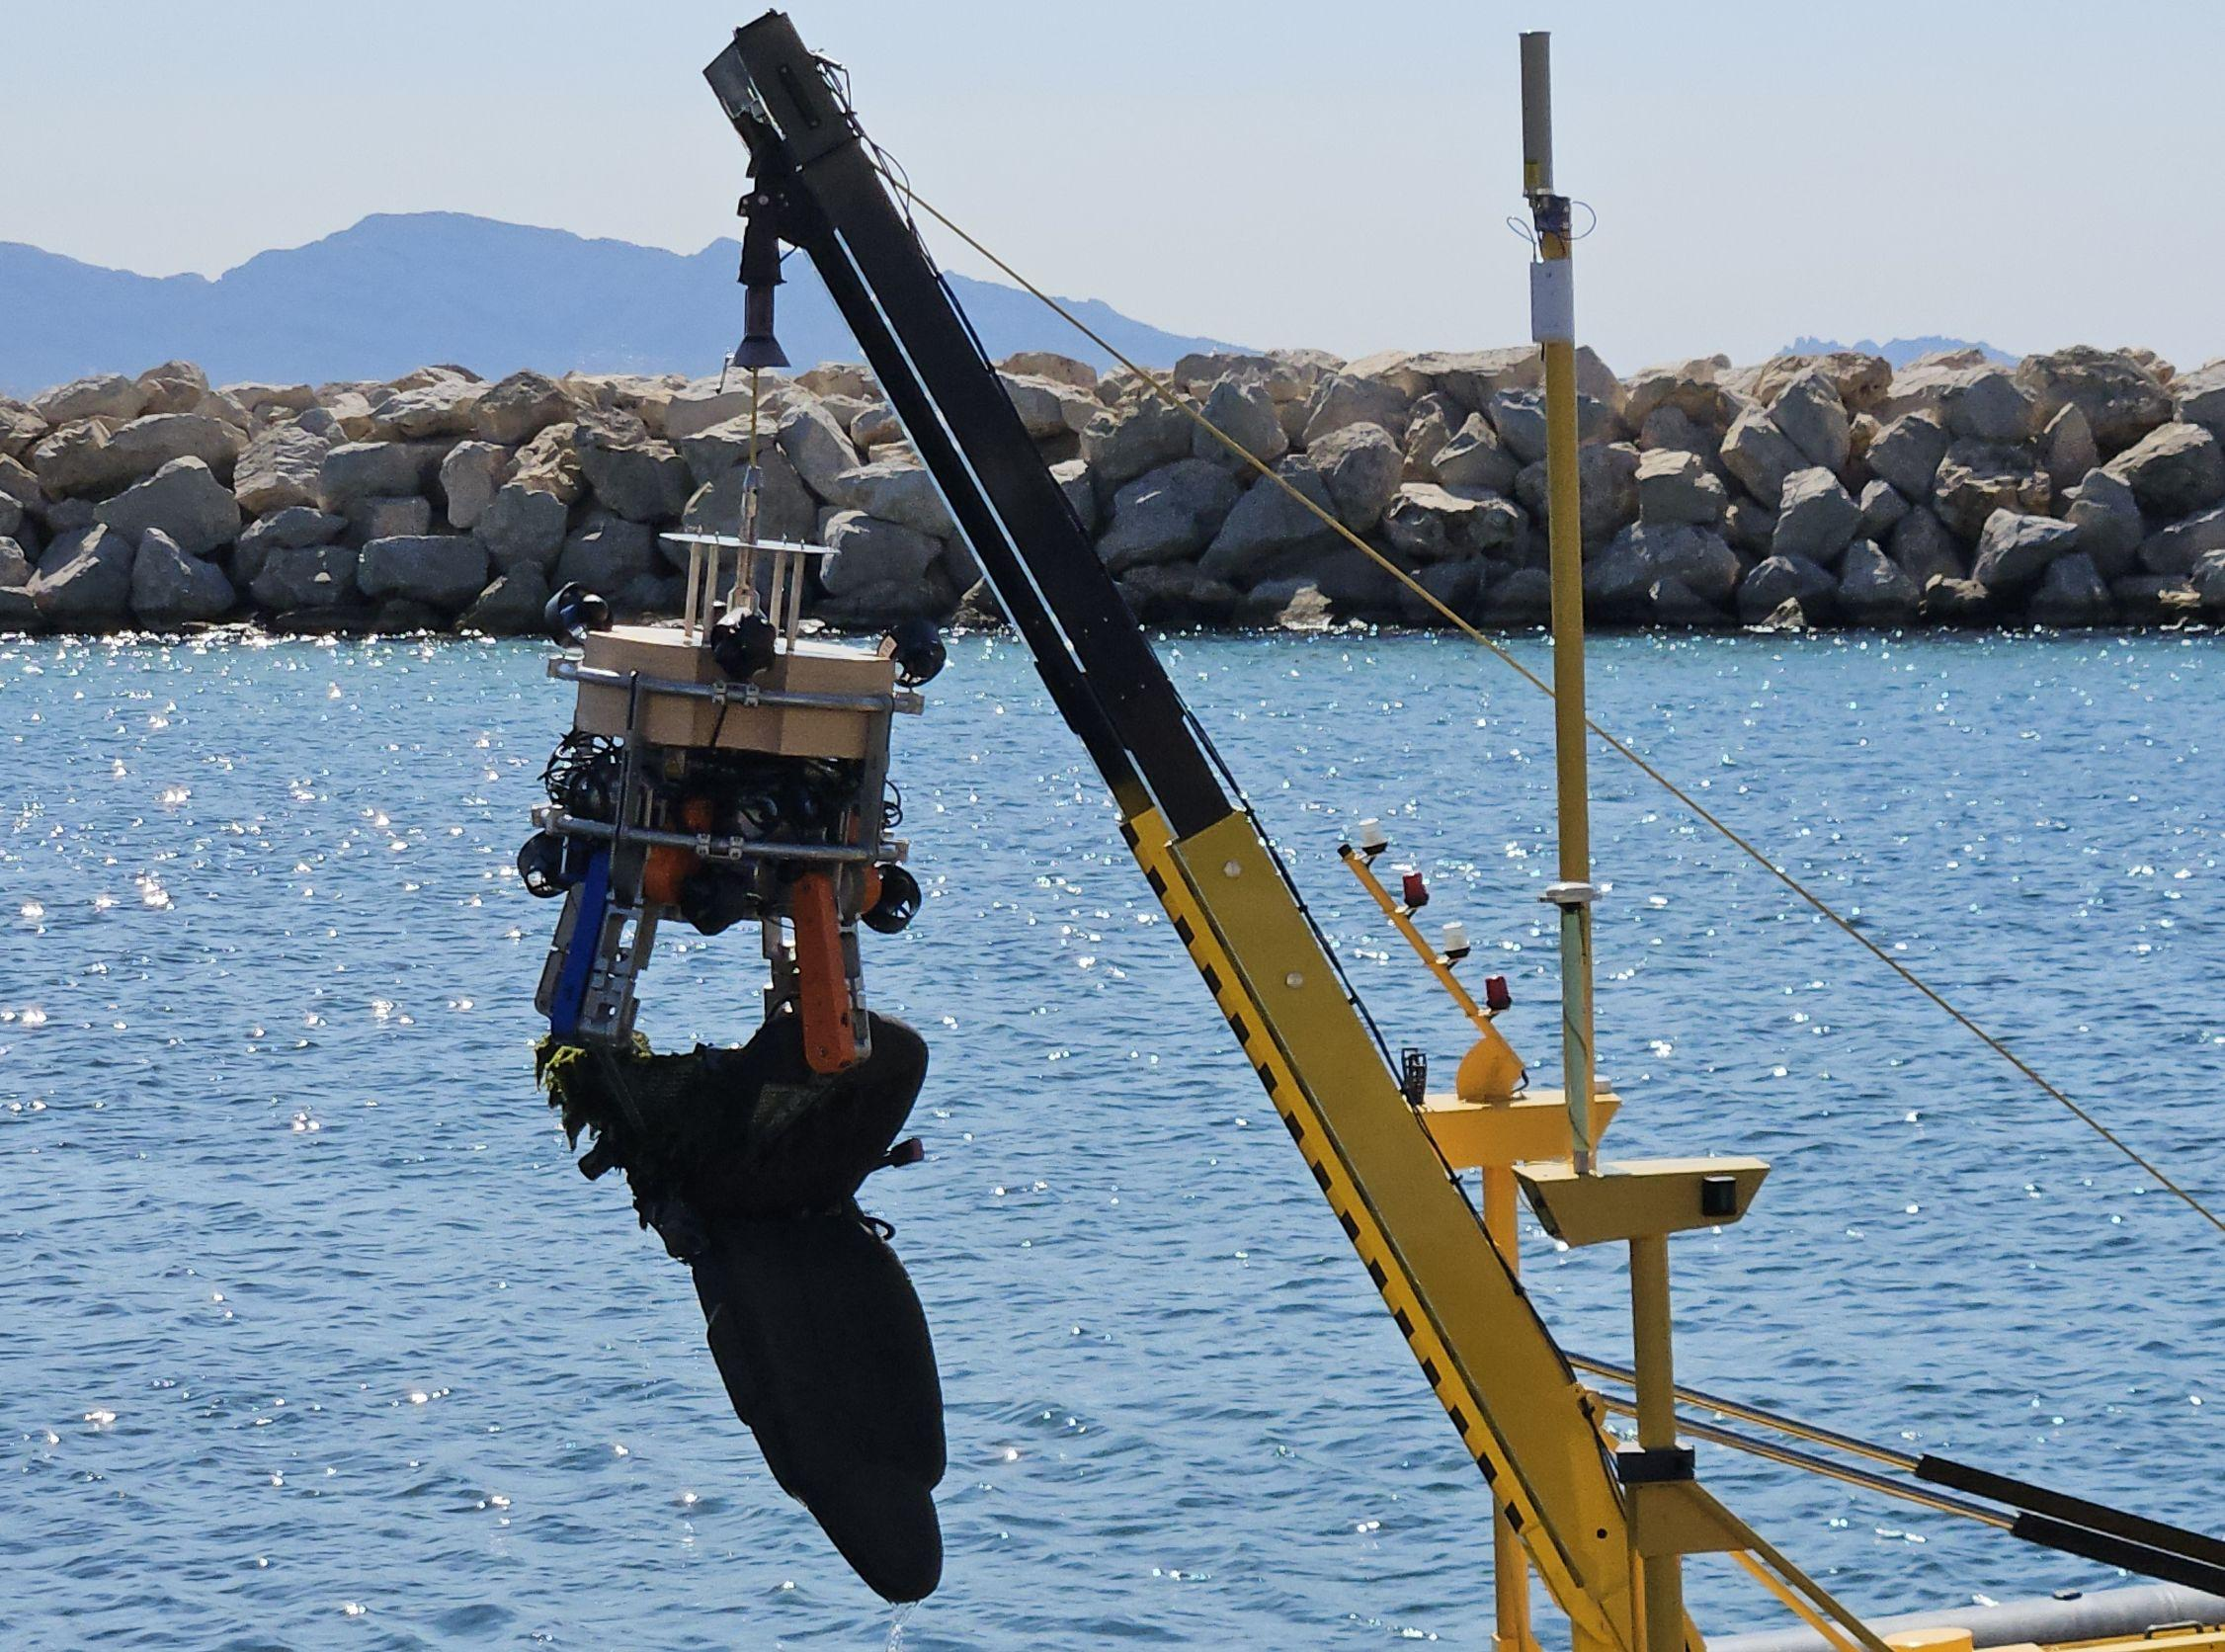
\includegraphics[width=\textwidth, trim={0cm 1cm 0cm 0.5cm}, clip]{img/seaclear_car_seat.jpeg}
        \caption{View from the control center.}
        \label{fig:ctrl_center_cam}
    \end{subfigure}
    %----------------------------------------------------------
    \caption{Grasping of a car seat during the media demo day in Marseille, September 2025.}
    \label{fig:grasping_cam}
\end{figure}


\begin{figure}[!h]
    \centering
    %----------------------------------------------------------
    \begin{subfigure}[t]{0.48\textwidth}
        \centering
        % Crop left, bottom, right, top (adjust as needed)
        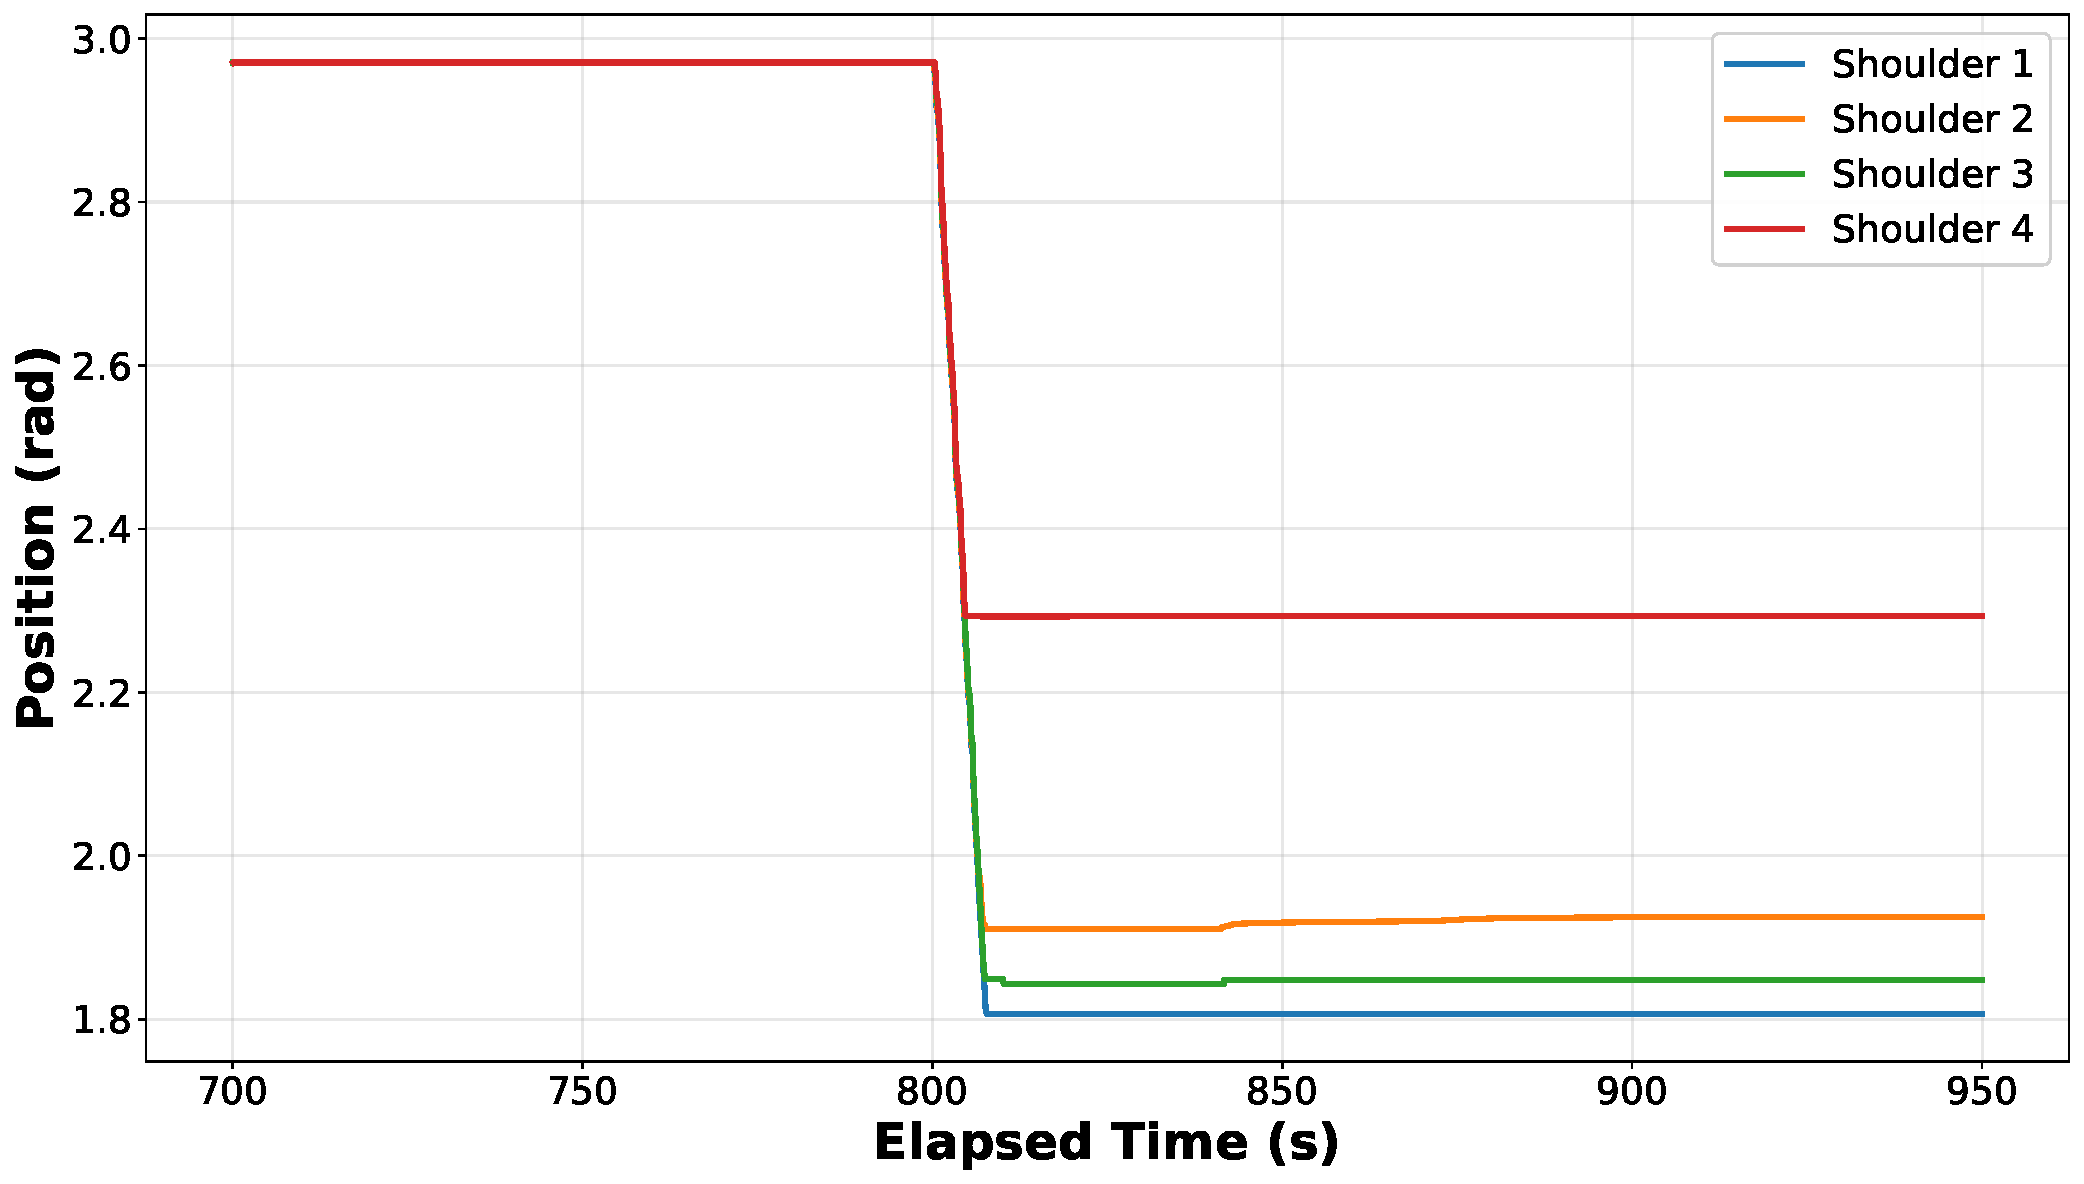
\includegraphics[width=\textwidth]{img/shoulder_joint_positions.pdf}
        \caption{Shoulder joint positions [rad].}
        \label{fig:shoulder_positions}
    \end{subfigure}
    \hfill
    %----------------------------------------------------------
    \begin{subfigure}[t]{0.48\textwidth}
        \centering
        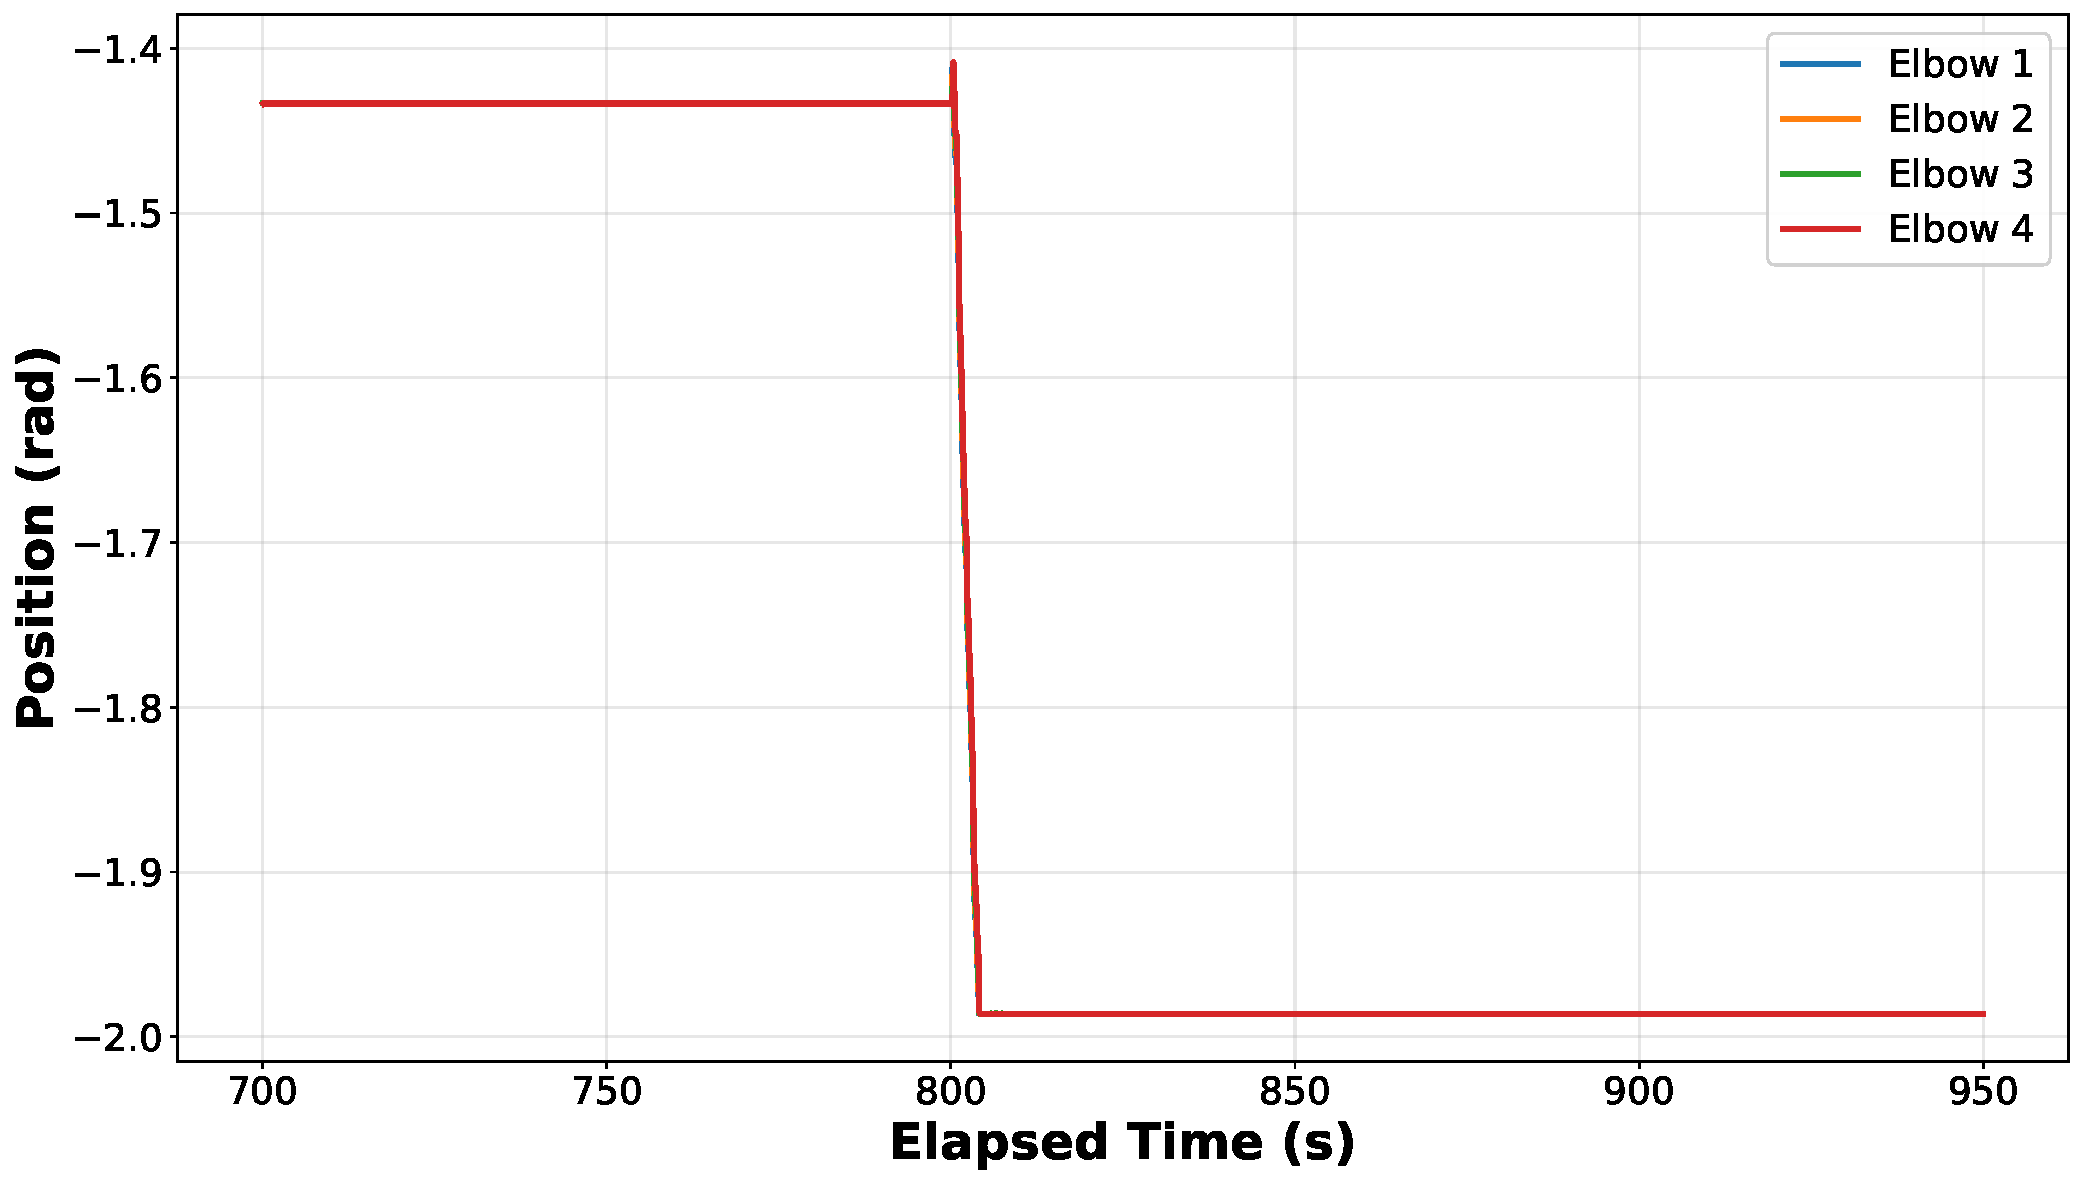
\includegraphics[width=\textwidth]{img/elbow_joint_positions.pdf}
        \caption{Elbow joint positions [rad].}
        \label{fig:elbow_positions}
    \end{subfigure}
    %----------------------------------------------------------
    \caption{Closing motion of the \gls{usg} to grasp the car seat. The joint positions can be related to the reference frame introduced in Figure~\ref{fig:grapple_kinematics}. The \gls{usg} begins to grasp around \(t \approx 800\,\mathrm{s}\).}
    \label{fig:joint_position_overview}
\end{figure}

\begin{figure}
    \centering
    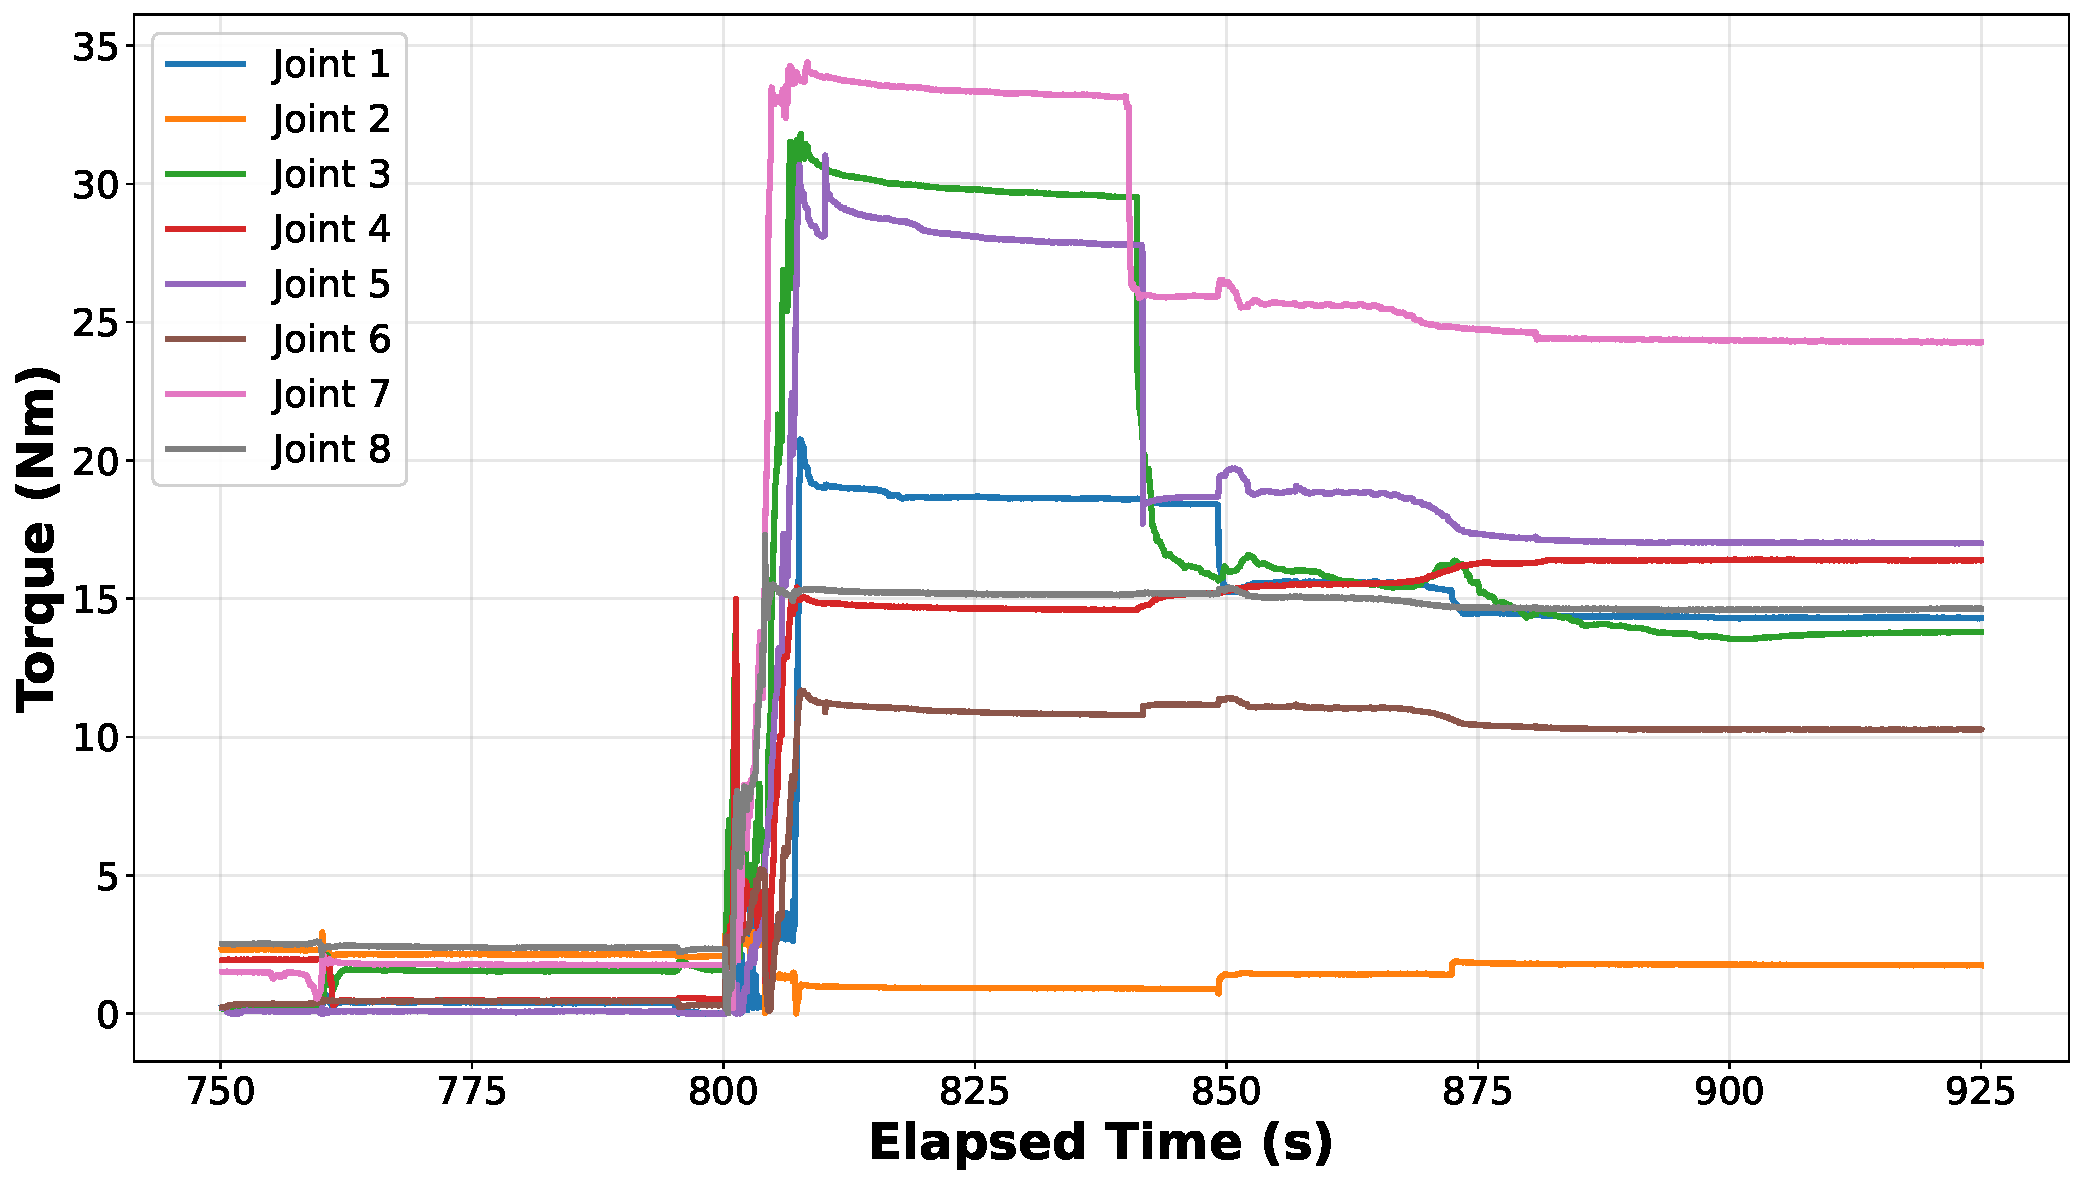
\includegraphics[width=0.8\linewidth]{img/all_joint_torques.pdf}
    \caption{Joint torque profiles during the grasping maneuver, showing a clear increase shortly after \(t \approx 800\,\mathrm{s}\) once there is contact with the car seat.}
    \label{fig:joint_torques}
\end{figure}

Besides grasping smaller objects, such as the car seat (and, in separate trials, a tire), an attempt to grasp a larger piece of shipwreck was also conducted successfully, as seen in Figure~\ref{fig:ship_wreck}, although the contact area was too large to recover it completely from the water.

\begin{figure}
    \centering
    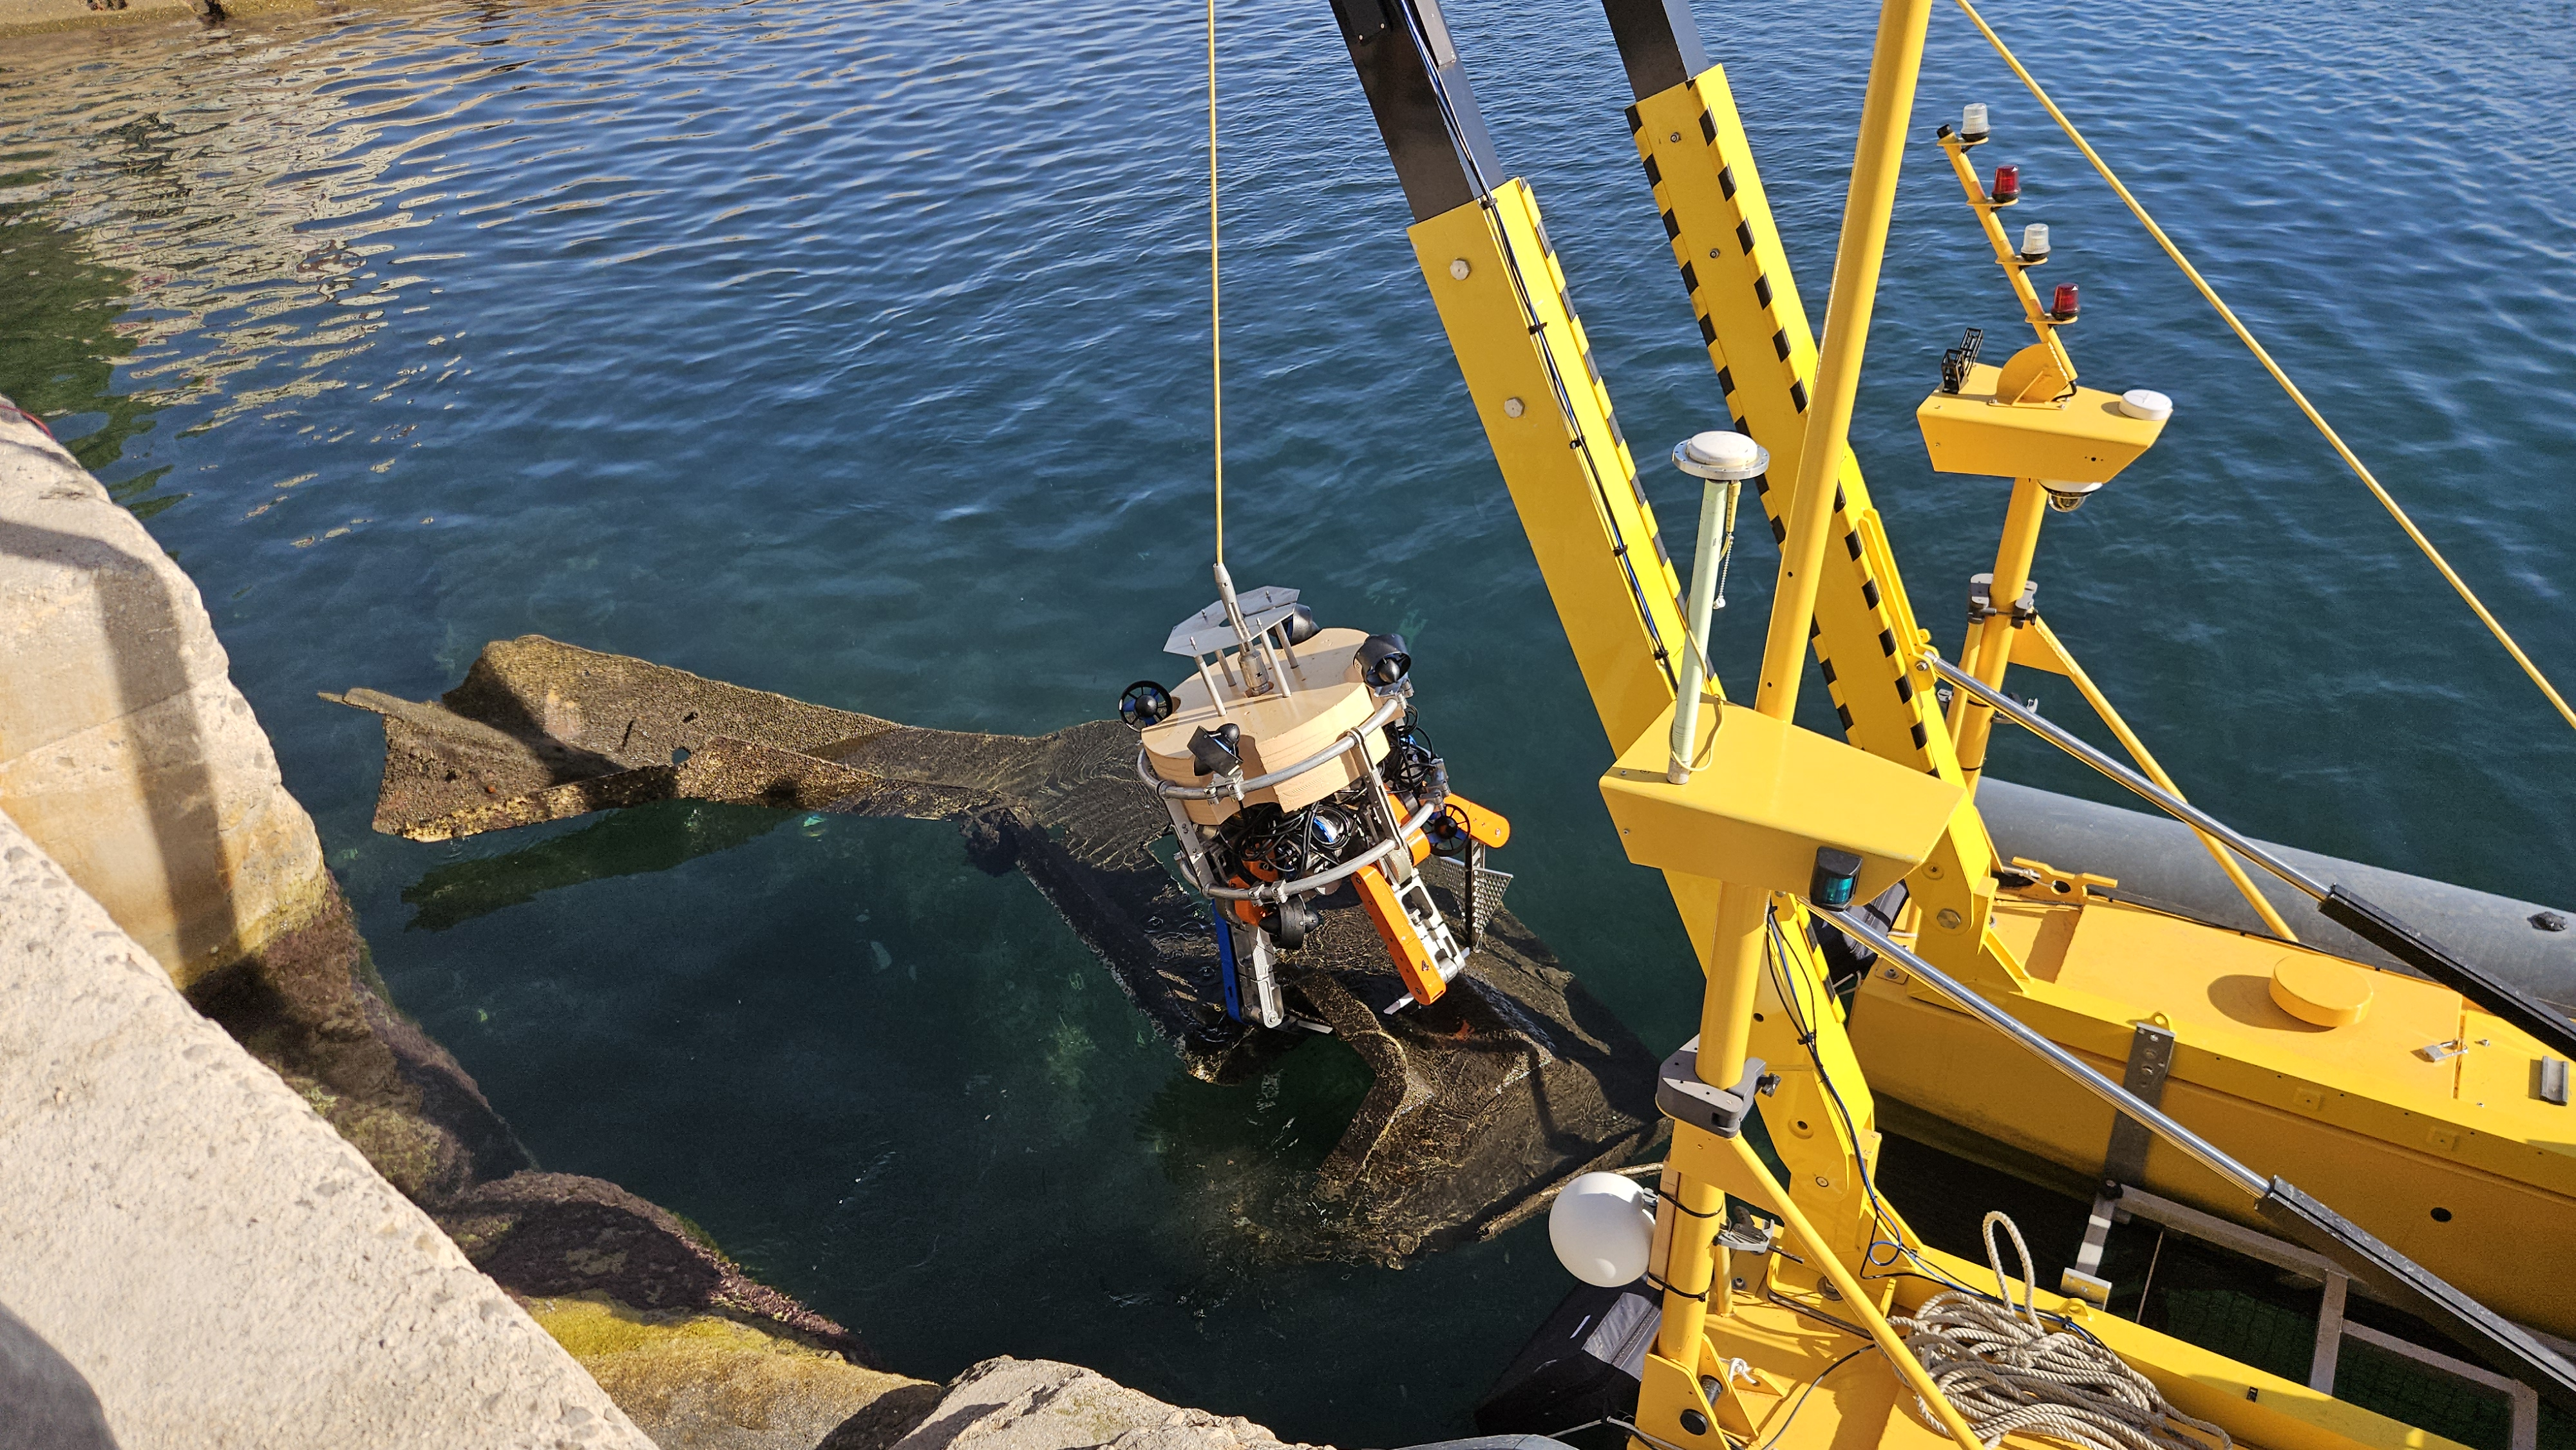
\includegraphics[width=0.8\linewidth]{img/ship_wreck.jpg}
    \caption{Attempted grasp of a shipwreck fragment during the media demo day.}
    \label{fig:ship_wreck}
\end{figure}


%%%%%%%%%%%%%%%%%%%%%%%%%%%%%%%%%%%%%%%%%%%%%%%%
% Section break
\section{Conclusions}

This deliverable successfully documents a comprehensive software framework for the SeaClear2.0 Smart Grapple system, demonstrating significant advances of the system for autonomous underwater manipulation for marine litter collection. The integrated approach combines a  holistic optimal control, robust state estimation, adaptive grasping algorithms, and real-time perception.
Key accomplishments include validated grasping capability for objects up to 250 kg, successful field demonstrations in Marseille 2025, and a modular software architecture enabling both autonomous and manual operation modes. The system's ability to handle environmental disturbances through stochastic optimal control and feedback augmentation addresses critical challenges in underwater robotics.
Future work should focus on improving computational efficiency of the trajectory optimization (currently requiring 4-17 hours), enhancing visual servoing for poor visibility conditions, and further integration testing of the complete autonomous operation cycle. The digital twin infrastructure provides a solid foundation for continued development between sea trials.

%%%%%%%%%%%%%%%%%%%%%%%%%%%%%%%%%%%%%%%%%%%%%%%%
\bibliographystyle{IEEEtran}
\bibliography{bib/literature}
\addcontentsline{toc}{section}{References}

%%%%%%%%%%%%%%%%%%%%%%%%%%%%%%%%%%%%%%%%%%%%%%%%
% % Appendix, if required
 \appendix
\section{Parameter lists}
% \addcontentsline{toc}{section}{Annex A: Parameter lists}

\subsection{Thrust allocation} \label{appendix:thrustalloc}

\begin{table}[h!]
\centering
\caption{Nominal thruster positions and orientation angles (Blue Robotics T500). 
Note the $90^\circ$ increments in $\psi_z$ around $+\!Z_{\mathrm{ref}}$ (see Figure \ref{fig:thruster_overview}) between consecutive thrusters.}
\begin{tabular}{c|c|rrr|rrrr}
\toprule
Thruster & VESC ID & \multicolumn{3}{c|}{Nominal position $\vec{p}_i$ [m]} &
\multicolumn{4}{c}{Angles [deg]}\\
\midrule
 &  & $p_x$ & $p_y$ & $p_z$ &
 $\theta_y$ & $\theta_z$ & $\theta_x$ & $\psi_z$ \\
\midrule
1 & 16  &  0.23586 & -0.23906 & -0.13283 & -45 & 45 & -180 &  -54 \\
2 & 140 &  0.23586 &  0.23906 & -0.13283 & -45 & 45 & -180 &   36 \\
3 & 132 & -0.23586 &  0.23906 & -0.13283 & -45 & 45 & -180 &  126 \\
4 & 40  & -0.23586 & -0.23906 & -0.13283 & -45 & 45 & -180 &  216 \\
5 & 32  &  0.23586 & -0.23906 &  0.34903 & -45 & 45 &  -90 &  -54 \\
6 & 124 &  0.23586 &  0.23906 &  0.34903 & -45 & 45 &  -90 &   36 \\
7 & 116 & -0.23586 &  0.23906 &  0.34903 & -45 & 45 &  -90 &  126 \\
8 & 24  & -0.23586 & -0.23906 &  0.34903 & -45 & 45 &  -90 &  216 \\
\bottomrule
\end{tabular}
\label{tab:thruster_pose_nominal_vesc}
\end{table}

\subsection{Kinematic parameters}

\begin{table}[h!]
\centering
\caption{The kinematic parameters of the smart grapple system.}
\begin{tabularx}{\linewidth}{l r X}
        \toprule
        \textbf{Parameter} & \textbf{Value} &  \textbf{Description} \\
        \midrule
        $l_1$ & 323.09 mm & the first link of the finger \\
        $l_2$ & 381.40 mm & the second link of the finger \\
        $x_0$ & 280 mm & $x$ base position of the finger\\
        $y_0$ & 0 mm & $y$ base position of the finger\\
        \bottomrule
    \end{tabularx}
\label{tab:grapple_kinematics}
\end{table}

\newpage

 \subsection{Holistic control approach simulation parameters} \label{appendix:simparameters}

\begin{table}[h!]
    \centering
    \caption{List of relevant parameters to the simulation}
    \label{tab:Parameters}
    \begin{tabularx}{\linewidth}{l r r X}
        \toprule
        \textbf{Parameter} & \textbf{Value} & \textbf{Uncertainty} & \textbf{Description} \\
         & (Mean) & (Std. Dev.) & \\
        \midrule
        $m_{\text{USG}}$ & $210$\,kg & $73$\,kg & Mass of the \gls{usg} ($120$\,kg) + payload sampled from Weibull distribution with $\lambda = 100$ and shape $k = 1.5$ \\
        $m_{\text{USG,water}}$ & $90$\,kg & $31$\,kg & Apparent mass of \gls{usg} underwater \\
        $m_{\text{USV}}$ & $1300$\,kg & --- & Mass of SeaCAT (no LARS, full fuel tanks) \\
        $\vec{\eta}_{\text{USG}}$ & $[120, 120, 120,$ $0, 0, 0]^T$ & --- & \gls{usg} friction coefficients (kg$\cdot$s/m$^2$) \\
        $\vec{\eta}_{\text{USV}}$ & $[120, 120, 120,$ $0, 0, 0]^T$ & --- & \gls{usv} friction coefficients (kg$\cdot$s/m$^2$) \\
        $\eta_{l}$ & $300$\,kg/s & --- & Friction coefficient for the winch \\
        $\alpha$ & $0.1$ & --- & Risk parameter \\
        $\Delta T$ & $20$\,ms & --- & Simulation discretization time step \\
        $T_{\Delta}$ & $50$ & --- & Multiplicity factor between simulation timestep and control input steps \\
        $S_T$ & $120$ & --- & Number of control input timesteps \\
        $N_{\text{max,iter}}$ & $600$ & --- & Maximum number of iterations \\
        \bottomrule
    \end{tabularx}
\end{table}



\end{document}
